\documentclass[twoside]{book}

% Packages required by doxygen
\usepackage{fixltx2e}
\usepackage{calc}
\usepackage{doxygen}
\usepackage[export]{adjustbox} % also loads graphicx
\usepackage{graphicx}
\usepackage[utf8]{inputenc}
\usepackage{makeidx}
\usepackage{multicol}
\usepackage{multirow}
\PassOptionsToPackage{warn}{textcomp}
\usepackage{textcomp}
\usepackage[nointegrals]{wasysym}
\usepackage[table]{xcolor}

% Font selection
\usepackage[T1]{fontenc}
\usepackage[scaled=.90]{helvet}
\usepackage{courier}
\usepackage{amssymb}
\usepackage{sectsty}
\renewcommand{\familydefault}{\sfdefault}
\allsectionsfont{%
  \fontseries{bc}\selectfont%
  \color{darkgray}%
}
\renewcommand{\DoxyLabelFont}{%
  \fontseries{bc}\selectfont%
  \color{darkgray}%
}
\newcommand{\+}{\discretionary{\mbox{\scriptsize$\hookleftarrow$}}{}{}}

% Page & text layout
\usepackage{geometry}
\geometry{%
  a4paper,%
  top=2.5cm,%
  bottom=2.5cm,%
  left=2.5cm,%
  right=2.5cm%
}
\tolerance=750
\hfuzz=15pt
\hbadness=750
\setlength{\emergencystretch}{15pt}
\setlength{\parindent}{0cm}
\setlength{\parskip}{3ex plus 2ex minus 2ex}
\makeatletter
\renewcommand{\paragraph}{%
  \@startsection{paragraph}{4}{0ex}{-1.0ex}{1.0ex}{%
    \normalfont\normalsize\bfseries\SS@parafont%
  }%
}
\renewcommand{\subparagraph}{%
  \@startsection{subparagraph}{5}{0ex}{-1.0ex}{1.0ex}{%
    \normalfont\normalsize\bfseries\SS@subparafont%
  }%
}
\makeatother

% Headers & footers
\usepackage{fancyhdr}
\pagestyle{fancyplain}
\fancyhead[LE]{\fancyplain{}{\bfseries\thepage}}
\fancyhead[CE]{\fancyplain{}{}}
\fancyhead[RE]{\fancyplain{}{\bfseries\leftmark}}
\fancyhead[LO]{\fancyplain{}{\bfseries\rightmark}}
\fancyhead[CO]{\fancyplain{}{}}
\fancyhead[RO]{\fancyplain{}{\bfseries\thepage}}
\fancyfoot[LE]{\fancyplain{}{}}
\fancyfoot[CE]{\fancyplain{}{}}
\fancyfoot[RE]{\fancyplain{}{\bfseries\scriptsize Generated by Doxygen }}
\fancyfoot[LO]{\fancyplain{}{\bfseries\scriptsize Generated by Doxygen }}
\fancyfoot[CO]{\fancyplain{}{}}
\fancyfoot[RO]{\fancyplain{}{}}
\renewcommand{\footrulewidth}{0.4pt}
\renewcommand{\chaptermark}[1]{%
  \markboth{#1}{}%
}
\renewcommand{\sectionmark}[1]{%
  \markright{\thesection\ #1}%
}

% Indices & bibliography
\usepackage{natbib}
\usepackage[titles]{tocloft}
\setcounter{tocdepth}{3}
\setcounter{secnumdepth}{5}
\makeindex

% Hyperlinks (required, but should be loaded last)
\usepackage{ifpdf}
\ifpdf
  \usepackage[pdftex,pagebackref=true]{hyperref}
\else
  \usepackage[ps2pdf,pagebackref=true]{hyperref}
\fi
\hypersetup{%
  colorlinks=true,%
  linkcolor=blue,%
  citecolor=blue,%
  unicode%
}

% Custom commands
\newcommand{\clearemptydoublepage}{%
  \newpage{\pagestyle{empty}\cleardoublepage}%
}

\usepackage{caption}
\captionsetup{labelsep=space,justification=centering,font={bf},singlelinecheck=off,skip=4pt,position=top}

%===== C O N T E N T S =====

\begin{document}

% Titlepage & ToC
\hypersetup{pageanchor=false,
             bookmarksnumbered=true,
             pdfencoding=unicode
            }
\pagenumbering{roman}
\begin{titlepage}
\vspace*{7cm}
\begin{center}%
{\Large P\+PL Assignment \\[1ex]\large v1.\+0 }\\
\vspace*{1cm}
{\large Generated by Doxygen 1.8.11}\\
\end{center}
\end{titlepage}
\clearemptydoublepage
\tableofcontents
\clearemptydoublepage
\pagenumbering{arabic}
\hypersetup{pageanchor=true}

%--- Begin generated contents ---
\chapter{P\+PL Assignment}
\label{md_README}
\hypertarget{md_README}{}
i 
\chapter{Namespace Index}
\section{Namespace List}
Here is a list of all namespaces with brief descriptions\+:\begin{DoxyCompactList}
\item\contentsline{section}{\hyperlink{namespaceValentinePrimeTime}{Valentine\+Prime\+Time} }{\pageref{namespaceValentinePrimeTime}}{}
\end{DoxyCompactList}

\chapter{Class Index}
\section{Class List}
Here are the classes, structs, unions and interfaces with brief descriptions\+:\begin{DoxyCompactList}
\item\contentsline{section}{\hyperlink{classValentinePrimeTime_1_1ChoosyGirls}{Valentine\+Prime\+Time\+::\+Choosy\+Girls} }{\pageref{classValentinePrimeTime_1_1ChoosyGirls}}{}
\item\contentsline{section}{\hyperlink{classValentinePrimeTime_1_1DesperateGirls}{Valentine\+Prime\+Time\+::\+Desperate\+Girls} }{\pageref{classValentinePrimeTime_1_1DesperateGirls}}{}
\item\contentsline{section}{\hyperlink{classValentinePrimeTime_1_1EssentialGifts}{Valentine\+Prime\+Time\+::\+Essential\+Gifts} }{\pageref{classValentinePrimeTime_1_1EssentialGifts}}{}
\item\contentsline{section}{\hyperlink{classValentinePrimeTime_1_1GeekBoys}{Valentine\+Prime\+Time\+::\+Geek\+Boys} }{\pageref{classValentinePrimeTime_1_1GeekBoys}}{}
\item\contentsline{section}{\hyperlink{classValentinePrimeTime_1_1GenerousBoys}{Valentine\+Prime\+Time\+::\+Generous\+Boys} }{\pageref{classValentinePrimeTime_1_1GenerousBoys}}{}
\item\contentsline{section}{\hyperlink{classValentinePrimeTime_1_1GiftRecord}{Valentine\+Prime\+Time\+::\+Gift\+Record} }{\pageref{classValentinePrimeTime_1_1GiftRecord}}{}
\item\contentsline{section}{\hyperlink{classValentinePrimeTime_1_1LuxuryGifts}{Valentine\+Prime\+Time\+::\+Luxury\+Gifts} }{\pageref{classValentinePrimeTime_1_1LuxuryGifts}}{}
\item\contentsline{section}{\hyperlink{classValentinePrimeTime_1_1MiserBoys}{Valentine\+Prime\+Time\+::\+Miser\+Boys} }{\pageref{classValentinePrimeTime_1_1MiserBoys}}{}
\item\contentsline{section}{\hyperlink{classValentinePrimeTime_1_1NormalGirls}{Valentine\+Prime\+Time\+::\+Normal\+Girls} }{\pageref{classValentinePrimeTime_1_1NormalGirls}}{}
\item\contentsline{section}{\hyperlink{classValentinePrimeTime_1_1Relationship}{Valentine\+Prime\+Time\+::\+Relationship} }{\pageref{classValentinePrimeTime_1_1Relationship}}{}
\item\contentsline{section}{\hyperlink{classValentinePrimeTime_1_1UtilityGifts}{Valentine\+Prime\+Time\+::\+Utility\+Gifts} }{\pageref{classValentinePrimeTime_1_1UtilityGifts}}{}
\end{DoxyCompactList}

\chapter{File Index}
\section{File List}
Here is a list of all files with brief descriptions\+:\begin{DoxyCompactList}
\item\contentsline{section}{\hyperlink{ChoosyGirls_8cpp}{Choosy\+Girls.\+cpp} }{\pageref{ChoosyGirls_8cpp}}{}
\item\contentsline{section}{\hyperlink{ChoosyGirls_8hpp}{Choosy\+Girls.\+hpp} }{\pageref{ChoosyGirls_8hpp}}{}
\item\contentsline{section}{\hyperlink{DesperateGirls_8cpp}{Desperate\+Girls.\+cpp} }{\pageref{DesperateGirls_8cpp}}{}
\item\contentsline{section}{\hyperlink{DesperateGirls_8hpp}{Desperate\+Girls.\+hpp} }{\pageref{DesperateGirls_8hpp}}{}
\item\contentsline{section}{\hyperlink{EssentialGifts_8cpp}{Essential\+Gifts.\+cpp} }{\pageref{EssentialGifts_8cpp}}{}
\item\contentsline{section}{\hyperlink{EssentialGifts_8hpp}{Essential\+Gifts.\+hpp} }{\pageref{EssentialGifts_8hpp}}{}
\item\contentsline{section}{\hyperlink{GeekBoys_8cpp}{Geek\+Boys.\+cpp} }{\pageref{GeekBoys_8cpp}}{}
\item\contentsline{section}{\hyperlink{GeekBoys_8hpp}{Geek\+Boys.\+hpp} }{\pageref{GeekBoys_8hpp}}{}
\item\contentsline{section}{\hyperlink{GenerousBoys_8cpp}{Generous\+Boys.\+cpp} }{\pageref{GenerousBoys_8cpp}}{}
\item\contentsline{section}{\hyperlink{GenerousBoys_8hpp}{Generous\+Boys.\+hpp} }{\pageref{GenerousBoys_8hpp}}{}
\item\contentsline{section}{\hyperlink{GenTestData_8cpp}{Gen\+Test\+Data.\+cpp} }{\pageref{GenTestData_8cpp}}{}
\item\contentsline{section}{\hyperlink{GiftRecord_8cpp}{Gift\+Record.\+cpp} }{\pageref{GiftRecord_8cpp}}{}
\item\contentsline{section}{\hyperlink{GiftRecord_8hpp}{Gift\+Record.\+hpp} }{\pageref{GiftRecord_8hpp}}{}
\item\contentsline{section}{\hyperlink{LuxuryGifts_8cpp}{Luxury\+Gifts.\+cpp} }{\pageref{LuxuryGifts_8cpp}}{}
\item\contentsline{section}{\hyperlink{LuxuryGifts_8hpp}{Luxury\+Gifts.\+hpp} }{\pageref{LuxuryGifts_8hpp}}{}
\item\contentsline{section}{\hyperlink{MiserBoys_8cpp}{Miser\+Boys.\+cpp} }{\pageref{MiserBoys_8cpp}}{}
\item\contentsline{section}{\hyperlink{MiserBoys_8hpp}{Miser\+Boys.\+hpp} }{\pageref{MiserBoys_8hpp}}{}
\item\contentsline{section}{\hyperlink{NormalGirls_8cpp}{Normal\+Girls.\+cpp} }{\pageref{NormalGirls_8cpp}}{}
\item\contentsline{section}{\hyperlink{NormalGirls_8hpp}{Normal\+Girls.\+hpp} }{\pageref{NormalGirls_8hpp}}{}
\item\contentsline{section}{\hyperlink{Q1Main_8cpp}{Q1\+Main.\+cpp} }{\pageref{Q1Main_8cpp}}{}
\item\contentsline{section}{\hyperlink{Q2Main_8cpp}{Q2\+Main.\+cpp} }{\pageref{Q2Main_8cpp}}{}
\item\contentsline{section}{\hyperlink{randomGen_8cpp}{random\+Gen.\+cpp} }{\pageref{randomGen_8cpp}}{}
\item\contentsline{section}{\hyperlink{Relationship_8cpp}{Relationship.\+cpp} }{\pageref{Relationship_8cpp}}{}
\item\contentsline{section}{\hyperlink{Relationship_8hpp}{Relationship.\+hpp} }{\pageref{Relationship_8hpp}}{}
\item\contentsline{section}{\hyperlink{UtilityGifts_8cpp}{Utility\+Gifts.\+cpp} }{\pageref{UtilityGifts_8cpp}}{}
\item\contentsline{section}{\hyperlink{UtilityGifts_8hpp}{Utility\+Gifts.\+hpp} }{\pageref{UtilityGifts_8hpp}}{}
\end{DoxyCompactList}

\chapter{Namespace Documentation}
\hypertarget{namespaceValentinePrimeTime}{}\section{Valentine\+Prime\+Time Namespace Reference}
\label{namespaceValentinePrimeTime}\index{Valentine\+Prime\+Time@{Valentine\+Prime\+Time}}
\subsection*{Classes}
\begin{DoxyCompactItemize}
\item 
class \hyperlink{classValentinePrimeTime_1_1ChoosyGirls}{Choosy\+Girls}
\item 
class \hyperlink{classValentinePrimeTime_1_1DesperateGirls}{Desperate\+Girls}
\item 
class \hyperlink{classValentinePrimeTime_1_1EssentialGifts}{Essential\+Gifts}
\item 
class \hyperlink{classValentinePrimeTime_1_1GeekBoys}{Geek\+Boys}
\item 
class \hyperlink{classValentinePrimeTime_1_1GenerousBoys}{Generous\+Boys}
\item 
class \hyperlink{classValentinePrimeTime_1_1GiftRecord}{Gift\+Record}
\item 
class \hyperlink{classValentinePrimeTime_1_1LuxuryGifts}{Luxury\+Gifts}
\item 
class \hyperlink{classValentinePrimeTime_1_1MiserBoys}{Miser\+Boys}
\item 
class \hyperlink{classValentinePrimeTime_1_1NormalGirls}{Normal\+Girls}
\item 
class \hyperlink{classValentinePrimeTime_1_1Relationship}{Relationship}
\item 
class \hyperlink{classValentinePrimeTime_1_1UtilityGifts}{Utility\+Gifts}
\end{DoxyCompactItemize}

\chapter{Class Documentation}
\hypertarget{classValentinePrimeTime_1_1ChoosyGirls}{}\section{Valentine\+Prime\+Time\+:\+:Choosy\+Girls Class Reference}
\label{classValentinePrimeTime_1_1ChoosyGirls}\index{Valentine\+Prime\+Time\+::\+Choosy\+Girls@{Valentine\+Prime\+Time\+::\+Choosy\+Girls}}


{\ttfamily \#include $<$Choosy\+Girls.\+hpp$>$}

\subsection*{Public Member Functions}
\begin{DoxyCompactItemize}
\item 
std\+::string \hyperlink{classValentinePrimeTime_1_1ChoosyGirls_a6e8b42b08f63636d9cc1a8fd8af7d63e}{get\+Name} ()
\item 
void \hyperlink{classValentinePrimeTime_1_1ChoosyGirls_abc756845333790093c4f04314c50c664}{set\+Name} (std\+::string name)
\item 
double \hyperlink{classValentinePrimeTime_1_1ChoosyGirls_a793d9df2721e7cd24be525e233fa5914}{get\+Attractiveness} ()
\item 
void \hyperlink{classValentinePrimeTime_1_1ChoosyGirls_aabad788987433fe203f266a0be8c0150}{set\+Attractiveness} (double attractiveness)
\item 
double \hyperlink{classValentinePrimeTime_1_1ChoosyGirls_a3cbaa935bd54662044bbbd6035d44829}{get\+Intelligence\+Level} ()
\item 
void \hyperlink{classValentinePrimeTime_1_1ChoosyGirls_aae2126bcc6463c16e5cb4e3438058eee}{set\+Intelligence\+Level} (double intelligence\+Level)
\item 
int \hyperlink{classValentinePrimeTime_1_1ChoosyGirls_a82dd83e4949f9edf51d34b85f2be1c51}{get\+Maintenance\+Cost} ()
\item 
void \hyperlink{classValentinePrimeTime_1_1ChoosyGirls_ac97b429b6ebad4e62ef0d0ba8924e4e7}{set\+Maintenance\+Cost} (int maintenance\+Cost)
\item 
bool \hyperlink{classValentinePrimeTime_1_1ChoosyGirls_ada01ddf2a9ea40f51b52a17e6788ba51}{set\+Committed} (bool committed)
\item 
bool \hyperlink{classValentinePrimeTime_1_1ChoosyGirls_ae80f0aeed3c98838b20f235a2091473a}{get\+Committed} ()
\item 
int \hyperlink{classValentinePrimeTime_1_1ChoosyGirls_a9f96e75633947da1a4a3c08d4132f015}{happiness} (int cost)
\end{DoxyCompactItemize}


\subsection{Member Function Documentation}
\index{Valentine\+Prime\+Time\+::\+Choosy\+Girls@{Valentine\+Prime\+Time\+::\+Choosy\+Girls}!get\+Attractiveness@{get\+Attractiveness}}
\index{get\+Attractiveness@{get\+Attractiveness}!Valentine\+Prime\+Time\+::\+Choosy\+Girls@{Valentine\+Prime\+Time\+::\+Choosy\+Girls}}
\subsubsection[{\texorpdfstring{get\+Attractiveness()}{getAttractiveness()}}]{\setlength{\rightskip}{0pt plus 5cm}double Valentine\+Prime\+Time\+::\+Choosy\+Girls\+::get\+Attractiveness (
\begin{DoxyParamCaption}
{}
\end{DoxyParamCaption}
)}\hypertarget{classValentinePrimeTime_1_1ChoosyGirls_a793d9df2721e7cd24be525e233fa5914}{}\label{classValentinePrimeTime_1_1ChoosyGirls_a793d9df2721e7cd24be525e233fa5914}
\index{Valentine\+Prime\+Time\+::\+Choosy\+Girls@{Valentine\+Prime\+Time\+::\+Choosy\+Girls}!get\+Committed@{get\+Committed}}
\index{get\+Committed@{get\+Committed}!Valentine\+Prime\+Time\+::\+Choosy\+Girls@{Valentine\+Prime\+Time\+::\+Choosy\+Girls}}
\subsubsection[{\texorpdfstring{get\+Committed()}{getCommitted()}}]{\setlength{\rightskip}{0pt plus 5cm}bool Valentine\+Prime\+Time\+::\+Choosy\+Girls\+::get\+Committed (
\begin{DoxyParamCaption}
{}
\end{DoxyParamCaption}
)}\hypertarget{classValentinePrimeTime_1_1ChoosyGirls_ae80f0aeed3c98838b20f235a2091473a}{}\label{classValentinePrimeTime_1_1ChoosyGirls_ae80f0aeed3c98838b20f235a2091473a}
\index{Valentine\+Prime\+Time\+::\+Choosy\+Girls@{Valentine\+Prime\+Time\+::\+Choosy\+Girls}!get\+Intelligence\+Level@{get\+Intelligence\+Level}}
\index{get\+Intelligence\+Level@{get\+Intelligence\+Level}!Valentine\+Prime\+Time\+::\+Choosy\+Girls@{Valentine\+Prime\+Time\+::\+Choosy\+Girls}}
\subsubsection[{\texorpdfstring{get\+Intelligence\+Level()}{getIntelligenceLevel()}}]{\setlength{\rightskip}{0pt plus 5cm}double Valentine\+Prime\+Time\+::\+Choosy\+Girls\+::get\+Intelligence\+Level (
\begin{DoxyParamCaption}
{}
\end{DoxyParamCaption}
)}\hypertarget{classValentinePrimeTime_1_1ChoosyGirls_a3cbaa935bd54662044bbbd6035d44829}{}\label{classValentinePrimeTime_1_1ChoosyGirls_a3cbaa935bd54662044bbbd6035d44829}
\index{Valentine\+Prime\+Time\+::\+Choosy\+Girls@{Valentine\+Prime\+Time\+::\+Choosy\+Girls}!get\+Maintenance\+Cost@{get\+Maintenance\+Cost}}
\index{get\+Maintenance\+Cost@{get\+Maintenance\+Cost}!Valentine\+Prime\+Time\+::\+Choosy\+Girls@{Valentine\+Prime\+Time\+::\+Choosy\+Girls}}
\subsubsection[{\texorpdfstring{get\+Maintenance\+Cost()}{getMaintenanceCost()}}]{\setlength{\rightskip}{0pt plus 5cm}int Valentine\+Prime\+Time\+::\+Choosy\+Girls\+::get\+Maintenance\+Cost (
\begin{DoxyParamCaption}
{}
\end{DoxyParamCaption}
)}\hypertarget{classValentinePrimeTime_1_1ChoosyGirls_a82dd83e4949f9edf51d34b85f2be1c51}{}\label{classValentinePrimeTime_1_1ChoosyGirls_a82dd83e4949f9edf51d34b85f2be1c51}
\index{Valentine\+Prime\+Time\+::\+Choosy\+Girls@{Valentine\+Prime\+Time\+::\+Choosy\+Girls}!get\+Name@{get\+Name}}
\index{get\+Name@{get\+Name}!Valentine\+Prime\+Time\+::\+Choosy\+Girls@{Valentine\+Prime\+Time\+::\+Choosy\+Girls}}
\subsubsection[{\texorpdfstring{get\+Name()}{getName()}}]{\setlength{\rightskip}{0pt plus 5cm}std\+::string Valentine\+Prime\+Time\+::\+Choosy\+Girls\+::get\+Name (
\begin{DoxyParamCaption}
{}
\end{DoxyParamCaption}
)}\hypertarget{classValentinePrimeTime_1_1ChoosyGirls_a6e8b42b08f63636d9cc1a8fd8af7d63e}{}\label{classValentinePrimeTime_1_1ChoosyGirls_a6e8b42b08f63636d9cc1a8fd8af7d63e}
\index{Valentine\+Prime\+Time\+::\+Choosy\+Girls@{Valentine\+Prime\+Time\+::\+Choosy\+Girls}!happiness@{happiness}}
\index{happiness@{happiness}!Valentine\+Prime\+Time\+::\+Choosy\+Girls@{Valentine\+Prime\+Time\+::\+Choosy\+Girls}}
\subsubsection[{\texorpdfstring{happiness(int cost)}{happiness(int cost)}}]{\setlength{\rightskip}{0pt plus 5cm}int Valentine\+Prime\+Time\+::\+Choosy\+Girls\+::happiness (
\begin{DoxyParamCaption}
\item[{int}]{cost}
\end{DoxyParamCaption}
)}\hypertarget{classValentinePrimeTime_1_1ChoosyGirls_a9f96e75633947da1a4a3c08d4132f015}{}\label{classValentinePrimeTime_1_1ChoosyGirls_a9f96e75633947da1a4a3c08d4132f015}
\index{Valentine\+Prime\+Time\+::\+Choosy\+Girls@{Valentine\+Prime\+Time\+::\+Choosy\+Girls}!set\+Attractiveness@{set\+Attractiveness}}
\index{set\+Attractiveness@{set\+Attractiveness}!Valentine\+Prime\+Time\+::\+Choosy\+Girls@{Valentine\+Prime\+Time\+::\+Choosy\+Girls}}
\subsubsection[{\texorpdfstring{set\+Attractiveness(double attractiveness)}{setAttractiveness(double attractiveness)}}]{\setlength{\rightskip}{0pt plus 5cm}void Valentine\+Prime\+Time\+::\+Choosy\+Girls\+::set\+Attractiveness (
\begin{DoxyParamCaption}
\item[{double}]{attractiveness}
\end{DoxyParamCaption}
)}\hypertarget{classValentinePrimeTime_1_1ChoosyGirls_aabad788987433fe203f266a0be8c0150}{}\label{classValentinePrimeTime_1_1ChoosyGirls_aabad788987433fe203f266a0be8c0150}
\index{Valentine\+Prime\+Time\+::\+Choosy\+Girls@{Valentine\+Prime\+Time\+::\+Choosy\+Girls}!set\+Committed@{set\+Committed}}
\index{set\+Committed@{set\+Committed}!Valentine\+Prime\+Time\+::\+Choosy\+Girls@{Valentine\+Prime\+Time\+::\+Choosy\+Girls}}
\subsubsection[{\texorpdfstring{set\+Committed(bool committed)}{setCommitted(bool committed)}}]{\setlength{\rightskip}{0pt plus 5cm}bool Valentine\+Prime\+Time\+::\+Choosy\+Girls\+::set\+Committed (
\begin{DoxyParamCaption}
\item[{bool}]{committed}
\end{DoxyParamCaption}
)}\hypertarget{classValentinePrimeTime_1_1ChoosyGirls_ada01ddf2a9ea40f51b52a17e6788ba51}{}\label{classValentinePrimeTime_1_1ChoosyGirls_ada01ddf2a9ea40f51b52a17e6788ba51}
\index{Valentine\+Prime\+Time\+::\+Choosy\+Girls@{Valentine\+Prime\+Time\+::\+Choosy\+Girls}!set\+Intelligence\+Level@{set\+Intelligence\+Level}}
\index{set\+Intelligence\+Level@{set\+Intelligence\+Level}!Valentine\+Prime\+Time\+::\+Choosy\+Girls@{Valentine\+Prime\+Time\+::\+Choosy\+Girls}}
\subsubsection[{\texorpdfstring{set\+Intelligence\+Level(double intelligence\+Level)}{setIntelligenceLevel(double intelligenceLevel)}}]{\setlength{\rightskip}{0pt plus 5cm}void Valentine\+Prime\+Time\+::\+Choosy\+Girls\+::set\+Intelligence\+Level (
\begin{DoxyParamCaption}
\item[{double}]{intelligence\+Level}
\end{DoxyParamCaption}
)}\hypertarget{classValentinePrimeTime_1_1ChoosyGirls_aae2126bcc6463c16e5cb4e3438058eee}{}\label{classValentinePrimeTime_1_1ChoosyGirls_aae2126bcc6463c16e5cb4e3438058eee}
\index{Valentine\+Prime\+Time\+::\+Choosy\+Girls@{Valentine\+Prime\+Time\+::\+Choosy\+Girls}!set\+Maintenance\+Cost@{set\+Maintenance\+Cost}}
\index{set\+Maintenance\+Cost@{set\+Maintenance\+Cost}!Valentine\+Prime\+Time\+::\+Choosy\+Girls@{Valentine\+Prime\+Time\+::\+Choosy\+Girls}}
\subsubsection[{\texorpdfstring{set\+Maintenance\+Cost(int maintenance\+Cost)}{setMaintenanceCost(int maintenanceCost)}}]{\setlength{\rightskip}{0pt plus 5cm}void Valentine\+Prime\+Time\+::\+Choosy\+Girls\+::set\+Maintenance\+Cost (
\begin{DoxyParamCaption}
\item[{int}]{maintenance\+Cost}
\end{DoxyParamCaption}
)}\hypertarget{classValentinePrimeTime_1_1ChoosyGirls_ac97b429b6ebad4e62ef0d0ba8924e4e7}{}\label{classValentinePrimeTime_1_1ChoosyGirls_ac97b429b6ebad4e62ef0d0ba8924e4e7}
\index{Valentine\+Prime\+Time\+::\+Choosy\+Girls@{Valentine\+Prime\+Time\+::\+Choosy\+Girls}!set\+Name@{set\+Name}}
\index{set\+Name@{set\+Name}!Valentine\+Prime\+Time\+::\+Choosy\+Girls@{Valentine\+Prime\+Time\+::\+Choosy\+Girls}}
\subsubsection[{\texorpdfstring{set\+Name(std\+::string name)}{setName(std::string name)}}]{\setlength{\rightskip}{0pt plus 5cm}void Valentine\+Prime\+Time\+::\+Choosy\+Girls\+::set\+Name (
\begin{DoxyParamCaption}
\item[{std\+::string}]{name}
\end{DoxyParamCaption}
)}\hypertarget{classValentinePrimeTime_1_1ChoosyGirls_abc756845333790093c4f04314c50c664}{}\label{classValentinePrimeTime_1_1ChoosyGirls_abc756845333790093c4f04314c50c664}


The documentation for this class was generated from the following files\+:\begin{DoxyCompactItemize}
\item 
\hyperlink{ChoosyGirls_8hpp}{Choosy\+Girls.\+hpp}\item 
\hyperlink{ChoosyGirls_8cpp}{Choosy\+Girls.\+cpp}\end{DoxyCompactItemize}

\hypertarget{classValentinePrimeTime_1_1DesperateGirls}{}\section{Valentine\+Prime\+Time\+:\+:Desperate\+Girls Class Reference}
\label{classValentinePrimeTime_1_1DesperateGirls}\index{Valentine\+Prime\+Time\+::\+Desperate\+Girls@{Valentine\+Prime\+Time\+::\+Desperate\+Girls}}


{\ttfamily \#include $<$Desperate\+Girls.\+hpp$>$}

\subsection*{Public Member Functions}
\begin{DoxyCompactItemize}
\item 
std\+::string \hyperlink{classValentinePrimeTime_1_1DesperateGirls_ab571f4c85248b66956779db2b50223b2}{get\+Name} ()
\item 
void \hyperlink{classValentinePrimeTime_1_1DesperateGirls_a226957c5f2c682c3ad8f05bc7809a336}{set\+Name} (std\+::string name)
\item 
double \hyperlink{classValentinePrimeTime_1_1DesperateGirls_adc83beb72cb1e3860239f8c0e834aec9}{get\+Attractiveness} ()
\item 
void \hyperlink{classValentinePrimeTime_1_1DesperateGirls_ae3eb69eb885c5684f280482531c27ea7}{set\+Attractiveness} (double attractiveness)
\item 
double \hyperlink{classValentinePrimeTime_1_1DesperateGirls_a3b770a8c2e99298b265156fad9242842}{get\+Intelligence\+Level} ()
\item 
void \hyperlink{classValentinePrimeTime_1_1DesperateGirls_aa5d6bbe606f0e4bc8aa1b16f064e6d3e}{set\+Intelligence\+Level} (double intelligence\+Level)
\item 
int \hyperlink{classValentinePrimeTime_1_1DesperateGirls_ae59375aef119d322fb3c03fe0b2faa04}{get\+Maintenance\+Cost} ()
\item 
void \hyperlink{classValentinePrimeTime_1_1DesperateGirls_aa4648ae2b3997f5b5e743b2b8ff16369}{set\+Maintenance\+Cost} (int maintenance\+Cost)
\item 
bool \hyperlink{classValentinePrimeTime_1_1DesperateGirls_a8488574d99818a9a8ab689570745a4fe}{set\+Committed} (bool committed)
\item 
bool \hyperlink{classValentinePrimeTime_1_1DesperateGirls_af6fca5df53e1b32147ca2b578464f8bd}{get\+Committed} ()
\item 
int \hyperlink{classValentinePrimeTime_1_1DesperateGirls_a39540b0893ca3251cfedcae1763f0dbc}{happiness} (int cost)
\end{DoxyCompactItemize}


\subsection{Member Function Documentation}
\index{Valentine\+Prime\+Time\+::\+Desperate\+Girls@{Valentine\+Prime\+Time\+::\+Desperate\+Girls}!get\+Attractiveness@{get\+Attractiveness}}
\index{get\+Attractiveness@{get\+Attractiveness}!Valentine\+Prime\+Time\+::\+Desperate\+Girls@{Valentine\+Prime\+Time\+::\+Desperate\+Girls}}
\subsubsection[{\texorpdfstring{get\+Attractiveness()}{getAttractiveness()}}]{\setlength{\rightskip}{0pt plus 5cm}double Valentine\+Prime\+Time\+::\+Desperate\+Girls\+::get\+Attractiveness (
\begin{DoxyParamCaption}
{}
\end{DoxyParamCaption}
)}\hypertarget{classValentinePrimeTime_1_1DesperateGirls_adc83beb72cb1e3860239f8c0e834aec9}{}\label{classValentinePrimeTime_1_1DesperateGirls_adc83beb72cb1e3860239f8c0e834aec9}
\index{Valentine\+Prime\+Time\+::\+Desperate\+Girls@{Valentine\+Prime\+Time\+::\+Desperate\+Girls}!get\+Committed@{get\+Committed}}
\index{get\+Committed@{get\+Committed}!Valentine\+Prime\+Time\+::\+Desperate\+Girls@{Valentine\+Prime\+Time\+::\+Desperate\+Girls}}
\subsubsection[{\texorpdfstring{get\+Committed()}{getCommitted()}}]{\setlength{\rightskip}{0pt plus 5cm}bool Valentine\+Prime\+Time\+::\+Desperate\+Girls\+::get\+Committed (
\begin{DoxyParamCaption}
{}
\end{DoxyParamCaption}
)}\hypertarget{classValentinePrimeTime_1_1DesperateGirls_af6fca5df53e1b32147ca2b578464f8bd}{}\label{classValentinePrimeTime_1_1DesperateGirls_af6fca5df53e1b32147ca2b578464f8bd}
\index{Valentine\+Prime\+Time\+::\+Desperate\+Girls@{Valentine\+Prime\+Time\+::\+Desperate\+Girls}!get\+Intelligence\+Level@{get\+Intelligence\+Level}}
\index{get\+Intelligence\+Level@{get\+Intelligence\+Level}!Valentine\+Prime\+Time\+::\+Desperate\+Girls@{Valentine\+Prime\+Time\+::\+Desperate\+Girls}}
\subsubsection[{\texorpdfstring{get\+Intelligence\+Level()}{getIntelligenceLevel()}}]{\setlength{\rightskip}{0pt plus 5cm}double Valentine\+Prime\+Time\+::\+Desperate\+Girls\+::get\+Intelligence\+Level (
\begin{DoxyParamCaption}
{}
\end{DoxyParamCaption}
)}\hypertarget{classValentinePrimeTime_1_1DesperateGirls_a3b770a8c2e99298b265156fad9242842}{}\label{classValentinePrimeTime_1_1DesperateGirls_a3b770a8c2e99298b265156fad9242842}
\index{Valentine\+Prime\+Time\+::\+Desperate\+Girls@{Valentine\+Prime\+Time\+::\+Desperate\+Girls}!get\+Maintenance\+Cost@{get\+Maintenance\+Cost}}
\index{get\+Maintenance\+Cost@{get\+Maintenance\+Cost}!Valentine\+Prime\+Time\+::\+Desperate\+Girls@{Valentine\+Prime\+Time\+::\+Desperate\+Girls}}
\subsubsection[{\texorpdfstring{get\+Maintenance\+Cost()}{getMaintenanceCost()}}]{\setlength{\rightskip}{0pt plus 5cm}int Valentine\+Prime\+Time\+::\+Desperate\+Girls\+::get\+Maintenance\+Cost (
\begin{DoxyParamCaption}
{}
\end{DoxyParamCaption}
)}\hypertarget{classValentinePrimeTime_1_1DesperateGirls_ae59375aef119d322fb3c03fe0b2faa04}{}\label{classValentinePrimeTime_1_1DesperateGirls_ae59375aef119d322fb3c03fe0b2faa04}
\index{Valentine\+Prime\+Time\+::\+Desperate\+Girls@{Valentine\+Prime\+Time\+::\+Desperate\+Girls}!get\+Name@{get\+Name}}
\index{get\+Name@{get\+Name}!Valentine\+Prime\+Time\+::\+Desperate\+Girls@{Valentine\+Prime\+Time\+::\+Desperate\+Girls}}
\subsubsection[{\texorpdfstring{get\+Name()}{getName()}}]{\setlength{\rightskip}{0pt plus 5cm}std\+::string Valentine\+Prime\+Time\+::\+Desperate\+Girls\+::get\+Name (
\begin{DoxyParamCaption}
{}
\end{DoxyParamCaption}
)}\hypertarget{classValentinePrimeTime_1_1DesperateGirls_ab571f4c85248b66956779db2b50223b2}{}\label{classValentinePrimeTime_1_1DesperateGirls_ab571f4c85248b66956779db2b50223b2}
\index{Valentine\+Prime\+Time\+::\+Desperate\+Girls@{Valentine\+Prime\+Time\+::\+Desperate\+Girls}!happiness@{happiness}}
\index{happiness@{happiness}!Valentine\+Prime\+Time\+::\+Desperate\+Girls@{Valentine\+Prime\+Time\+::\+Desperate\+Girls}}
\subsubsection[{\texorpdfstring{happiness(int cost)}{happiness(int cost)}}]{\setlength{\rightskip}{0pt plus 5cm}int Valentine\+Prime\+Time\+::\+Desperate\+Girls\+::happiness (
\begin{DoxyParamCaption}
\item[{int}]{cost}
\end{DoxyParamCaption}
)}\hypertarget{classValentinePrimeTime_1_1DesperateGirls_a39540b0893ca3251cfedcae1763f0dbc}{}\label{classValentinePrimeTime_1_1DesperateGirls_a39540b0893ca3251cfedcae1763f0dbc}
\index{Valentine\+Prime\+Time\+::\+Desperate\+Girls@{Valentine\+Prime\+Time\+::\+Desperate\+Girls}!set\+Attractiveness@{set\+Attractiveness}}
\index{set\+Attractiveness@{set\+Attractiveness}!Valentine\+Prime\+Time\+::\+Desperate\+Girls@{Valentine\+Prime\+Time\+::\+Desperate\+Girls}}
\subsubsection[{\texorpdfstring{set\+Attractiveness(double attractiveness)}{setAttractiveness(double attractiveness)}}]{\setlength{\rightskip}{0pt plus 5cm}void Valentine\+Prime\+Time\+::\+Desperate\+Girls\+::set\+Attractiveness (
\begin{DoxyParamCaption}
\item[{double}]{attractiveness}
\end{DoxyParamCaption}
)}\hypertarget{classValentinePrimeTime_1_1DesperateGirls_ae3eb69eb885c5684f280482531c27ea7}{}\label{classValentinePrimeTime_1_1DesperateGirls_ae3eb69eb885c5684f280482531c27ea7}
\index{Valentine\+Prime\+Time\+::\+Desperate\+Girls@{Valentine\+Prime\+Time\+::\+Desperate\+Girls}!set\+Committed@{set\+Committed}}
\index{set\+Committed@{set\+Committed}!Valentine\+Prime\+Time\+::\+Desperate\+Girls@{Valentine\+Prime\+Time\+::\+Desperate\+Girls}}
\subsubsection[{\texorpdfstring{set\+Committed(bool committed)}{setCommitted(bool committed)}}]{\setlength{\rightskip}{0pt plus 5cm}bool Valentine\+Prime\+Time\+::\+Desperate\+Girls\+::set\+Committed (
\begin{DoxyParamCaption}
\item[{bool}]{committed}
\end{DoxyParamCaption}
)}\hypertarget{classValentinePrimeTime_1_1DesperateGirls_a8488574d99818a9a8ab689570745a4fe}{}\label{classValentinePrimeTime_1_1DesperateGirls_a8488574d99818a9a8ab689570745a4fe}
\index{Valentine\+Prime\+Time\+::\+Desperate\+Girls@{Valentine\+Prime\+Time\+::\+Desperate\+Girls}!set\+Intelligence\+Level@{set\+Intelligence\+Level}}
\index{set\+Intelligence\+Level@{set\+Intelligence\+Level}!Valentine\+Prime\+Time\+::\+Desperate\+Girls@{Valentine\+Prime\+Time\+::\+Desperate\+Girls}}
\subsubsection[{\texorpdfstring{set\+Intelligence\+Level(double intelligence\+Level)}{setIntelligenceLevel(double intelligenceLevel)}}]{\setlength{\rightskip}{0pt plus 5cm}void Valentine\+Prime\+Time\+::\+Desperate\+Girls\+::set\+Intelligence\+Level (
\begin{DoxyParamCaption}
\item[{double}]{intelligence\+Level}
\end{DoxyParamCaption}
)}\hypertarget{classValentinePrimeTime_1_1DesperateGirls_aa5d6bbe606f0e4bc8aa1b16f064e6d3e}{}\label{classValentinePrimeTime_1_1DesperateGirls_aa5d6bbe606f0e4bc8aa1b16f064e6d3e}
\index{Valentine\+Prime\+Time\+::\+Desperate\+Girls@{Valentine\+Prime\+Time\+::\+Desperate\+Girls}!set\+Maintenance\+Cost@{set\+Maintenance\+Cost}}
\index{set\+Maintenance\+Cost@{set\+Maintenance\+Cost}!Valentine\+Prime\+Time\+::\+Desperate\+Girls@{Valentine\+Prime\+Time\+::\+Desperate\+Girls}}
\subsubsection[{\texorpdfstring{set\+Maintenance\+Cost(int maintenance\+Cost)}{setMaintenanceCost(int maintenanceCost)}}]{\setlength{\rightskip}{0pt plus 5cm}void Valentine\+Prime\+Time\+::\+Desperate\+Girls\+::set\+Maintenance\+Cost (
\begin{DoxyParamCaption}
\item[{int}]{maintenance\+Cost}
\end{DoxyParamCaption}
)}\hypertarget{classValentinePrimeTime_1_1DesperateGirls_aa4648ae2b3997f5b5e743b2b8ff16369}{}\label{classValentinePrimeTime_1_1DesperateGirls_aa4648ae2b3997f5b5e743b2b8ff16369}
\index{Valentine\+Prime\+Time\+::\+Desperate\+Girls@{Valentine\+Prime\+Time\+::\+Desperate\+Girls}!set\+Name@{set\+Name}}
\index{set\+Name@{set\+Name}!Valentine\+Prime\+Time\+::\+Desperate\+Girls@{Valentine\+Prime\+Time\+::\+Desperate\+Girls}}
\subsubsection[{\texorpdfstring{set\+Name(std\+::string name)}{setName(std::string name)}}]{\setlength{\rightskip}{0pt plus 5cm}void Valentine\+Prime\+Time\+::\+Desperate\+Girls\+::set\+Name (
\begin{DoxyParamCaption}
\item[{std\+::string}]{name}
\end{DoxyParamCaption}
)}\hypertarget{classValentinePrimeTime_1_1DesperateGirls_a226957c5f2c682c3ad8f05bc7809a336}{}\label{classValentinePrimeTime_1_1DesperateGirls_a226957c5f2c682c3ad8f05bc7809a336}


The documentation for this class was generated from the following files\+:\begin{DoxyCompactItemize}
\item 
\hyperlink{DesperateGirls_8hpp}{Desperate\+Girls.\+hpp}\item 
\hyperlink{DesperateGirls_8cpp}{Desperate\+Girls.\+cpp}\end{DoxyCompactItemize}

\hypertarget{classValentinePrimeTime_1_1EssentialGifts}{}\section{Valentine\+Prime\+Time\+:\+:Essential\+Gifts Class Reference}
\label{classValentinePrimeTime_1_1EssentialGifts}\index{Valentine\+Prime\+Time\+::\+Essential\+Gifts@{Valentine\+Prime\+Time\+::\+Essential\+Gifts}}


{\ttfamily \#include $<$Essential\+Gifts.\+hpp$>$}

\subsection*{Public Member Functions}
\begin{DoxyCompactItemize}
\item 
std\+::string \hyperlink{classValentinePrimeTime_1_1EssentialGifts_a55fd1aaba0395e894882db2e48c85776}{get\+Name} ()
\item 
void \hyperlink{classValentinePrimeTime_1_1EssentialGifts_a77f380eac144b6be3e6aa8bafff587b9}{set\+Name} (std\+::string name)
\item 
int \hyperlink{classValentinePrimeTime_1_1EssentialGifts_a5d29916ed1a4579ea7da4e51a00f33c8}{get\+Price} ()
\item 
int \hyperlink{classValentinePrimeTime_1_1EssentialGifts_a64da4e14815c66aa38f028dc8c557097}{get\+Value} ()
\item 
void \hyperlink{classValentinePrimeTime_1_1EssentialGifts_a36e42e3c0eaf96e80ccd5ae3c5fb725d}{set\+Price} (int price)
\item 
void \hyperlink{classValentinePrimeTime_1_1EssentialGifts_a260ca8e3dc0544b0fdce8e4367c09b08}{set\+Value} (int value)
\end{DoxyCompactItemize}


\subsection{Member Function Documentation}
\index{Valentine\+Prime\+Time\+::\+Essential\+Gifts@{Valentine\+Prime\+Time\+::\+Essential\+Gifts}!get\+Name@{get\+Name}}
\index{get\+Name@{get\+Name}!Valentine\+Prime\+Time\+::\+Essential\+Gifts@{Valentine\+Prime\+Time\+::\+Essential\+Gifts}}
\subsubsection[{\texorpdfstring{get\+Name()}{getName()}}]{\setlength{\rightskip}{0pt plus 5cm}std\+::string Valentine\+Prime\+Time\+::\+Essential\+Gifts\+::get\+Name (
\begin{DoxyParamCaption}
{}
\end{DoxyParamCaption}
)}\hypertarget{classValentinePrimeTime_1_1EssentialGifts_a55fd1aaba0395e894882db2e48c85776}{}\label{classValentinePrimeTime_1_1EssentialGifts_a55fd1aaba0395e894882db2e48c85776}
\index{Valentine\+Prime\+Time\+::\+Essential\+Gifts@{Valentine\+Prime\+Time\+::\+Essential\+Gifts}!get\+Price@{get\+Price}}
\index{get\+Price@{get\+Price}!Valentine\+Prime\+Time\+::\+Essential\+Gifts@{Valentine\+Prime\+Time\+::\+Essential\+Gifts}}
\subsubsection[{\texorpdfstring{get\+Price()}{getPrice()}}]{\setlength{\rightskip}{0pt plus 5cm}int Valentine\+Prime\+Time\+::\+Essential\+Gifts\+::get\+Price (
\begin{DoxyParamCaption}
{}
\end{DoxyParamCaption}
)}\hypertarget{classValentinePrimeTime_1_1EssentialGifts_a5d29916ed1a4579ea7da4e51a00f33c8}{}\label{classValentinePrimeTime_1_1EssentialGifts_a5d29916ed1a4579ea7da4e51a00f33c8}
\index{Valentine\+Prime\+Time\+::\+Essential\+Gifts@{Valentine\+Prime\+Time\+::\+Essential\+Gifts}!get\+Value@{get\+Value}}
\index{get\+Value@{get\+Value}!Valentine\+Prime\+Time\+::\+Essential\+Gifts@{Valentine\+Prime\+Time\+::\+Essential\+Gifts}}
\subsubsection[{\texorpdfstring{get\+Value()}{getValue()}}]{\setlength{\rightskip}{0pt plus 5cm}int Valentine\+Prime\+Time\+::\+Essential\+Gifts\+::get\+Value (
\begin{DoxyParamCaption}
{}
\end{DoxyParamCaption}
)}\hypertarget{classValentinePrimeTime_1_1EssentialGifts_a64da4e14815c66aa38f028dc8c557097}{}\label{classValentinePrimeTime_1_1EssentialGifts_a64da4e14815c66aa38f028dc8c557097}
\index{Valentine\+Prime\+Time\+::\+Essential\+Gifts@{Valentine\+Prime\+Time\+::\+Essential\+Gifts}!set\+Name@{set\+Name}}
\index{set\+Name@{set\+Name}!Valentine\+Prime\+Time\+::\+Essential\+Gifts@{Valentine\+Prime\+Time\+::\+Essential\+Gifts}}
\subsubsection[{\texorpdfstring{set\+Name(std\+::string name)}{setName(std::string name)}}]{\setlength{\rightskip}{0pt plus 5cm}void Valentine\+Prime\+Time\+::\+Essential\+Gifts\+::set\+Name (
\begin{DoxyParamCaption}
\item[{std\+::string}]{name}
\end{DoxyParamCaption}
)}\hypertarget{classValentinePrimeTime_1_1EssentialGifts_a77f380eac144b6be3e6aa8bafff587b9}{}\label{classValentinePrimeTime_1_1EssentialGifts_a77f380eac144b6be3e6aa8bafff587b9}
\index{Valentine\+Prime\+Time\+::\+Essential\+Gifts@{Valentine\+Prime\+Time\+::\+Essential\+Gifts}!set\+Price@{set\+Price}}
\index{set\+Price@{set\+Price}!Valentine\+Prime\+Time\+::\+Essential\+Gifts@{Valentine\+Prime\+Time\+::\+Essential\+Gifts}}
\subsubsection[{\texorpdfstring{set\+Price(int price)}{setPrice(int price)}}]{\setlength{\rightskip}{0pt plus 5cm}void Valentine\+Prime\+Time\+::\+Essential\+Gifts\+::set\+Price (
\begin{DoxyParamCaption}
\item[{int}]{price}
\end{DoxyParamCaption}
)}\hypertarget{classValentinePrimeTime_1_1EssentialGifts_a36e42e3c0eaf96e80ccd5ae3c5fb725d}{}\label{classValentinePrimeTime_1_1EssentialGifts_a36e42e3c0eaf96e80ccd5ae3c5fb725d}
\index{Valentine\+Prime\+Time\+::\+Essential\+Gifts@{Valentine\+Prime\+Time\+::\+Essential\+Gifts}!set\+Value@{set\+Value}}
\index{set\+Value@{set\+Value}!Valentine\+Prime\+Time\+::\+Essential\+Gifts@{Valentine\+Prime\+Time\+::\+Essential\+Gifts}}
\subsubsection[{\texorpdfstring{set\+Value(int value)}{setValue(int value)}}]{\setlength{\rightskip}{0pt plus 5cm}void Valentine\+Prime\+Time\+::\+Essential\+Gifts\+::set\+Value (
\begin{DoxyParamCaption}
\item[{int}]{value}
\end{DoxyParamCaption}
)}\hypertarget{classValentinePrimeTime_1_1EssentialGifts_a260ca8e3dc0544b0fdce8e4367c09b08}{}\label{classValentinePrimeTime_1_1EssentialGifts_a260ca8e3dc0544b0fdce8e4367c09b08}


The documentation for this class was generated from the following files\+:\begin{DoxyCompactItemize}
\item 
\hyperlink{EssentialGifts_8hpp}{Essential\+Gifts.\+hpp}\item 
\hyperlink{EssentialGifts_8cpp}{Essential\+Gifts.\+cpp}\end{DoxyCompactItemize}

\hypertarget{classValentinePrimeTime_1_1GeekBoys}{}\section{Valentine\+Prime\+Time\+:\+:Geek\+Boys Class Reference}
\label{classValentinePrimeTime_1_1GeekBoys}\index{Valentine\+Prime\+Time\+::\+Geek\+Boys@{Valentine\+Prime\+Time\+::\+Geek\+Boys}}


{\ttfamily \#include $<$Geek\+Boys.\+hpp$>$}

\subsection*{Public Member Functions}
\begin{DoxyCompactItemize}
\item 
std\+::string \hyperlink{classValentinePrimeTime_1_1GeekBoys_a76f0a4ca28c7080b0f61aed0dc6ccaaf}{get\+Name} ()
\item 
void \hyperlink{classValentinePrimeTime_1_1GeekBoys_a269c0422f5897d9ee415534c4872a7dd}{set\+Name} (std\+::string name)
\item 
double \hyperlink{classValentinePrimeTime_1_1GeekBoys_aaef699271498a1f17f62ce0a9e3b095e}{get\+Attractiveness} ()
\item 
void \hyperlink{classValentinePrimeTime_1_1GeekBoys_ae2264065c398670653b725983389a27f}{set\+Attractiveness} (double attractiveness)
\item 
double \hyperlink{classValentinePrimeTime_1_1GeekBoys_a4a8a697c8866120e1c3605a8340e89e1}{get\+Intelligence\+Level} ()
\item 
void \hyperlink{classValentinePrimeTime_1_1GeekBoys_a39cc3df57069b06d60715a9f082976cd}{set\+Intelligence\+Level} (double intelligence\+Level)
\item 
int \hyperlink{classValentinePrimeTime_1_1GeekBoys_ad1574a8a5c76981bdb57f2abab9d2c35}{get\+Budget} ()
\item 
void \hyperlink{classValentinePrimeTime_1_1GeekBoys_ab601f93d180c36753dcf5398fc32e985}{set\+Budget} (int budget)
\item 
bool \hyperlink{classValentinePrimeTime_1_1GeekBoys_a052981302e69000e53f5c3d2df2389fc}{set\+Committed} (bool b)
\item 
bool \hyperlink{classValentinePrimeTime_1_1GeekBoys_a951ea4a43b0f8f6e1b364e75219078c7}{get\+Committed} ()
\item 
int \hyperlink{classValentinePrimeTime_1_1GeekBoys_abe862d56c9b17a1665a61bc5f88964c1}{happiness} ()
\item 
int \hyperlink{classValentinePrimeTime_1_1GeekBoys_acf94dccd9b17665e85729283e0967a00}{get\+Req\+Attraction} ()
\item 
void \hyperlink{classValentinePrimeTime_1_1GeekBoys_ad5e9658844f8704bb89cd3b41d8f5441}{set\+Req\+Attraction} (int at)
\end{DoxyCompactItemize}


\subsection{Member Function Documentation}
\index{Valentine\+Prime\+Time\+::\+Geek\+Boys@{Valentine\+Prime\+Time\+::\+Geek\+Boys}!get\+Attractiveness@{get\+Attractiveness}}
\index{get\+Attractiveness@{get\+Attractiveness}!Valentine\+Prime\+Time\+::\+Geek\+Boys@{Valentine\+Prime\+Time\+::\+Geek\+Boys}}
\subsubsection[{\texorpdfstring{get\+Attractiveness()}{getAttractiveness()}}]{\setlength{\rightskip}{0pt plus 5cm}double Valentine\+Prime\+Time\+::\+Geek\+Boys\+::get\+Attractiveness (
\begin{DoxyParamCaption}
{}
\end{DoxyParamCaption}
)}\hypertarget{classValentinePrimeTime_1_1GeekBoys_aaef699271498a1f17f62ce0a9e3b095e}{}\label{classValentinePrimeTime_1_1GeekBoys_aaef699271498a1f17f62ce0a9e3b095e}
\index{Valentine\+Prime\+Time\+::\+Geek\+Boys@{Valentine\+Prime\+Time\+::\+Geek\+Boys}!get\+Budget@{get\+Budget}}
\index{get\+Budget@{get\+Budget}!Valentine\+Prime\+Time\+::\+Geek\+Boys@{Valentine\+Prime\+Time\+::\+Geek\+Boys}}
\subsubsection[{\texorpdfstring{get\+Budget()}{getBudget()}}]{\setlength{\rightskip}{0pt plus 5cm}int Valentine\+Prime\+Time\+::\+Geek\+Boys\+::get\+Budget (
\begin{DoxyParamCaption}
{}
\end{DoxyParamCaption}
)}\hypertarget{classValentinePrimeTime_1_1GeekBoys_ad1574a8a5c76981bdb57f2abab9d2c35}{}\label{classValentinePrimeTime_1_1GeekBoys_ad1574a8a5c76981bdb57f2abab9d2c35}
\index{Valentine\+Prime\+Time\+::\+Geek\+Boys@{Valentine\+Prime\+Time\+::\+Geek\+Boys}!get\+Committed@{get\+Committed}}
\index{get\+Committed@{get\+Committed}!Valentine\+Prime\+Time\+::\+Geek\+Boys@{Valentine\+Prime\+Time\+::\+Geek\+Boys}}
\subsubsection[{\texorpdfstring{get\+Committed()}{getCommitted()}}]{\setlength{\rightskip}{0pt plus 5cm}bool Valentine\+Prime\+Time\+::\+Geek\+Boys\+::get\+Committed (
\begin{DoxyParamCaption}
{}
\end{DoxyParamCaption}
)}\hypertarget{classValentinePrimeTime_1_1GeekBoys_a951ea4a43b0f8f6e1b364e75219078c7}{}\label{classValentinePrimeTime_1_1GeekBoys_a951ea4a43b0f8f6e1b364e75219078c7}
\index{Valentine\+Prime\+Time\+::\+Geek\+Boys@{Valentine\+Prime\+Time\+::\+Geek\+Boys}!get\+Intelligence\+Level@{get\+Intelligence\+Level}}
\index{get\+Intelligence\+Level@{get\+Intelligence\+Level}!Valentine\+Prime\+Time\+::\+Geek\+Boys@{Valentine\+Prime\+Time\+::\+Geek\+Boys}}
\subsubsection[{\texorpdfstring{get\+Intelligence\+Level()}{getIntelligenceLevel()}}]{\setlength{\rightskip}{0pt plus 5cm}double Valentine\+Prime\+Time\+::\+Geek\+Boys\+::get\+Intelligence\+Level (
\begin{DoxyParamCaption}
{}
\end{DoxyParamCaption}
)}\hypertarget{classValentinePrimeTime_1_1GeekBoys_a4a8a697c8866120e1c3605a8340e89e1}{}\label{classValentinePrimeTime_1_1GeekBoys_a4a8a697c8866120e1c3605a8340e89e1}
\index{Valentine\+Prime\+Time\+::\+Geek\+Boys@{Valentine\+Prime\+Time\+::\+Geek\+Boys}!get\+Name@{get\+Name}}
\index{get\+Name@{get\+Name}!Valentine\+Prime\+Time\+::\+Geek\+Boys@{Valentine\+Prime\+Time\+::\+Geek\+Boys}}
\subsubsection[{\texorpdfstring{get\+Name()}{getName()}}]{\setlength{\rightskip}{0pt plus 5cm}std\+::string Valentine\+Prime\+Time\+::\+Geek\+Boys\+::get\+Name (
\begin{DoxyParamCaption}
{}
\end{DoxyParamCaption}
)}\hypertarget{classValentinePrimeTime_1_1GeekBoys_a76f0a4ca28c7080b0f61aed0dc6ccaaf}{}\label{classValentinePrimeTime_1_1GeekBoys_a76f0a4ca28c7080b0f61aed0dc6ccaaf}
\index{Valentine\+Prime\+Time\+::\+Geek\+Boys@{Valentine\+Prime\+Time\+::\+Geek\+Boys}!get\+Req\+Attraction@{get\+Req\+Attraction}}
\index{get\+Req\+Attraction@{get\+Req\+Attraction}!Valentine\+Prime\+Time\+::\+Geek\+Boys@{Valentine\+Prime\+Time\+::\+Geek\+Boys}}
\subsubsection[{\texorpdfstring{get\+Req\+Attraction()}{getReqAttraction()}}]{\setlength{\rightskip}{0pt plus 5cm}int Valentine\+Prime\+Time\+::\+Geek\+Boys\+::get\+Req\+Attraction (
\begin{DoxyParamCaption}
{}
\end{DoxyParamCaption}
)}\hypertarget{classValentinePrimeTime_1_1GeekBoys_acf94dccd9b17665e85729283e0967a00}{}\label{classValentinePrimeTime_1_1GeekBoys_acf94dccd9b17665e85729283e0967a00}
\index{Valentine\+Prime\+Time\+::\+Geek\+Boys@{Valentine\+Prime\+Time\+::\+Geek\+Boys}!happiness@{happiness}}
\index{happiness@{happiness}!Valentine\+Prime\+Time\+::\+Geek\+Boys@{Valentine\+Prime\+Time\+::\+Geek\+Boys}}
\subsubsection[{\texorpdfstring{happiness()}{happiness()}}]{\setlength{\rightskip}{0pt plus 5cm}int Valentine\+Prime\+Time\+::\+Geek\+Boys\+::happiness (
\begin{DoxyParamCaption}
{}
\end{DoxyParamCaption}
)}\hypertarget{classValentinePrimeTime_1_1GeekBoys_abe862d56c9b17a1665a61bc5f88964c1}{}\label{classValentinePrimeTime_1_1GeekBoys_abe862d56c9b17a1665a61bc5f88964c1}
\index{Valentine\+Prime\+Time\+::\+Geek\+Boys@{Valentine\+Prime\+Time\+::\+Geek\+Boys}!set\+Attractiveness@{set\+Attractiveness}}
\index{set\+Attractiveness@{set\+Attractiveness}!Valentine\+Prime\+Time\+::\+Geek\+Boys@{Valentine\+Prime\+Time\+::\+Geek\+Boys}}
\subsubsection[{\texorpdfstring{set\+Attractiveness(double attractiveness)}{setAttractiveness(double attractiveness)}}]{\setlength{\rightskip}{0pt plus 5cm}void Valentine\+Prime\+Time\+::\+Geek\+Boys\+::set\+Attractiveness (
\begin{DoxyParamCaption}
\item[{double}]{attractiveness}
\end{DoxyParamCaption}
)}\hypertarget{classValentinePrimeTime_1_1GeekBoys_ae2264065c398670653b725983389a27f}{}\label{classValentinePrimeTime_1_1GeekBoys_ae2264065c398670653b725983389a27f}
\index{Valentine\+Prime\+Time\+::\+Geek\+Boys@{Valentine\+Prime\+Time\+::\+Geek\+Boys}!set\+Budget@{set\+Budget}}
\index{set\+Budget@{set\+Budget}!Valentine\+Prime\+Time\+::\+Geek\+Boys@{Valentine\+Prime\+Time\+::\+Geek\+Boys}}
\subsubsection[{\texorpdfstring{set\+Budget(int budget)}{setBudget(int budget)}}]{\setlength{\rightskip}{0pt plus 5cm}void Valentine\+Prime\+Time\+::\+Geek\+Boys\+::set\+Budget (
\begin{DoxyParamCaption}
\item[{int}]{budget}
\end{DoxyParamCaption}
)}\hypertarget{classValentinePrimeTime_1_1GeekBoys_ab601f93d180c36753dcf5398fc32e985}{}\label{classValentinePrimeTime_1_1GeekBoys_ab601f93d180c36753dcf5398fc32e985}
\index{Valentine\+Prime\+Time\+::\+Geek\+Boys@{Valentine\+Prime\+Time\+::\+Geek\+Boys}!set\+Committed@{set\+Committed}}
\index{set\+Committed@{set\+Committed}!Valentine\+Prime\+Time\+::\+Geek\+Boys@{Valentine\+Prime\+Time\+::\+Geek\+Boys}}
\subsubsection[{\texorpdfstring{set\+Committed(bool b)}{setCommitted(bool b)}}]{\setlength{\rightskip}{0pt plus 5cm}bool Valentine\+Prime\+Time\+::\+Geek\+Boys\+::set\+Committed (
\begin{DoxyParamCaption}
\item[{bool}]{b}
\end{DoxyParamCaption}
)}\hypertarget{classValentinePrimeTime_1_1GeekBoys_a052981302e69000e53f5c3d2df2389fc}{}\label{classValentinePrimeTime_1_1GeekBoys_a052981302e69000e53f5c3d2df2389fc}
\index{Valentine\+Prime\+Time\+::\+Geek\+Boys@{Valentine\+Prime\+Time\+::\+Geek\+Boys}!set\+Intelligence\+Level@{set\+Intelligence\+Level}}
\index{set\+Intelligence\+Level@{set\+Intelligence\+Level}!Valentine\+Prime\+Time\+::\+Geek\+Boys@{Valentine\+Prime\+Time\+::\+Geek\+Boys}}
\subsubsection[{\texorpdfstring{set\+Intelligence\+Level(double intelligence\+Level)}{setIntelligenceLevel(double intelligenceLevel)}}]{\setlength{\rightskip}{0pt plus 5cm}void Valentine\+Prime\+Time\+::\+Geek\+Boys\+::set\+Intelligence\+Level (
\begin{DoxyParamCaption}
\item[{double}]{intelligence\+Level}
\end{DoxyParamCaption}
)}\hypertarget{classValentinePrimeTime_1_1GeekBoys_a39cc3df57069b06d60715a9f082976cd}{}\label{classValentinePrimeTime_1_1GeekBoys_a39cc3df57069b06d60715a9f082976cd}
\index{Valentine\+Prime\+Time\+::\+Geek\+Boys@{Valentine\+Prime\+Time\+::\+Geek\+Boys}!set\+Name@{set\+Name}}
\index{set\+Name@{set\+Name}!Valentine\+Prime\+Time\+::\+Geek\+Boys@{Valentine\+Prime\+Time\+::\+Geek\+Boys}}
\subsubsection[{\texorpdfstring{set\+Name(std\+::string name)}{setName(std::string name)}}]{\setlength{\rightskip}{0pt plus 5cm}void Valentine\+Prime\+Time\+::\+Geek\+Boys\+::set\+Name (
\begin{DoxyParamCaption}
\item[{std\+::string}]{name}
\end{DoxyParamCaption}
)}\hypertarget{classValentinePrimeTime_1_1GeekBoys_a269c0422f5897d9ee415534c4872a7dd}{}\label{classValentinePrimeTime_1_1GeekBoys_a269c0422f5897d9ee415534c4872a7dd}
\index{Valentine\+Prime\+Time\+::\+Geek\+Boys@{Valentine\+Prime\+Time\+::\+Geek\+Boys}!set\+Req\+Attraction@{set\+Req\+Attraction}}
\index{set\+Req\+Attraction@{set\+Req\+Attraction}!Valentine\+Prime\+Time\+::\+Geek\+Boys@{Valentine\+Prime\+Time\+::\+Geek\+Boys}}
\subsubsection[{\texorpdfstring{set\+Req\+Attraction(int at)}{setReqAttraction(int at)}}]{\setlength{\rightskip}{0pt plus 5cm}void Valentine\+Prime\+Time\+::\+Geek\+Boys\+::set\+Req\+Attraction (
\begin{DoxyParamCaption}
\item[{int}]{at}
\end{DoxyParamCaption}
)}\hypertarget{classValentinePrimeTime_1_1GeekBoys_ad5e9658844f8704bb89cd3b41d8f5441}{}\label{classValentinePrimeTime_1_1GeekBoys_ad5e9658844f8704bb89cd3b41d8f5441}


The documentation for this class was generated from the following files\+:\begin{DoxyCompactItemize}
\item 
\hyperlink{GeekBoys_8hpp}{Geek\+Boys.\+hpp}\item 
\hyperlink{GeekBoys_8cpp}{Geek\+Boys.\+cpp}\end{DoxyCompactItemize}

\hypertarget{classValentinePrimeTime_1_1GenerousBoys}{}\section{Valentine\+Prime\+Time\+:\+:Generous\+Boys Class Reference}
\label{classValentinePrimeTime_1_1GenerousBoys}\index{Valentine\+Prime\+Time\+::\+Generous\+Boys@{Valentine\+Prime\+Time\+::\+Generous\+Boys}}


{\ttfamily \#include $<$Generous\+Boys.\+hpp$>$}

\subsection*{Public Member Functions}
\begin{DoxyCompactItemize}
\item 
std\+::string \hyperlink{classValentinePrimeTime_1_1GenerousBoys_a681fc371c98927c6f56ce37557682dd3}{get\+Name} ()
\item 
void \hyperlink{classValentinePrimeTime_1_1GenerousBoys_af2617dc69ef73d8c6f4b609236b72d79}{set\+Name} (std\+::string name)
\item 
double \hyperlink{classValentinePrimeTime_1_1GenerousBoys_ac43244c2ede60fa83b3fdef2476fcadd}{get\+Attractiveness} ()
\item 
void \hyperlink{classValentinePrimeTime_1_1GenerousBoys_a3aac8c0df6bdf1366795d7e584cfda95}{set\+Attractiveness} (double attractiveness)
\item 
double \hyperlink{classValentinePrimeTime_1_1GenerousBoys_a66135371014278fdd3a4ceccf04b8be9}{get\+Intelligence\+Level} ()
\item 
void \hyperlink{classValentinePrimeTime_1_1GenerousBoys_acedc0ec40b4f53dac590b157859b4389}{set\+Intelligence\+Level} (double intelligence\+Level)
\item 
int \hyperlink{classValentinePrimeTime_1_1GenerousBoys_abdad37907ed9e9cfcd6be9783b6b9750}{get\+Budget} ()
\item 
void \hyperlink{classValentinePrimeTime_1_1GenerousBoys_ac97a0fc14d73c057b0028241469abbd2}{set\+Budget} (int budget)
\item 
bool \hyperlink{classValentinePrimeTime_1_1GenerousBoys_ab7dbd23d5a94c6a582d26022d53e2744}{set\+Committed} (bool b)
\item 
bool \hyperlink{classValentinePrimeTime_1_1GenerousBoys_aa57010d579dcba91069ccd3d9304ad27}{get\+Committed} ()
\item 
int \hyperlink{classValentinePrimeTime_1_1GenerousBoys_abc622283a3808904e3a93b0767c33dd0}{happiness} ()
\item 
int \hyperlink{classValentinePrimeTime_1_1GenerousBoys_a212c97cd61c3ed987df9c9c34318d416}{get\+Req\+Attraction} ()
\item 
void \hyperlink{classValentinePrimeTime_1_1GenerousBoys_ad76bf71f47634fde2ce07045a86b156a}{set\+Req\+Attraction} (int at)
\end{DoxyCompactItemize}


\subsection{Member Function Documentation}
\index{Valentine\+Prime\+Time\+::\+Generous\+Boys@{Valentine\+Prime\+Time\+::\+Generous\+Boys}!get\+Attractiveness@{get\+Attractiveness}}
\index{get\+Attractiveness@{get\+Attractiveness}!Valentine\+Prime\+Time\+::\+Generous\+Boys@{Valentine\+Prime\+Time\+::\+Generous\+Boys}}
\subsubsection[{\texorpdfstring{get\+Attractiveness()}{getAttractiveness()}}]{\setlength{\rightskip}{0pt plus 5cm}double Valentine\+Prime\+Time\+::\+Generous\+Boys\+::get\+Attractiveness (
\begin{DoxyParamCaption}
{}
\end{DoxyParamCaption}
)}\hypertarget{classValentinePrimeTime_1_1GenerousBoys_ac43244c2ede60fa83b3fdef2476fcadd}{}\label{classValentinePrimeTime_1_1GenerousBoys_ac43244c2ede60fa83b3fdef2476fcadd}
\index{Valentine\+Prime\+Time\+::\+Generous\+Boys@{Valentine\+Prime\+Time\+::\+Generous\+Boys}!get\+Budget@{get\+Budget}}
\index{get\+Budget@{get\+Budget}!Valentine\+Prime\+Time\+::\+Generous\+Boys@{Valentine\+Prime\+Time\+::\+Generous\+Boys}}
\subsubsection[{\texorpdfstring{get\+Budget()}{getBudget()}}]{\setlength{\rightskip}{0pt plus 5cm}int Valentine\+Prime\+Time\+::\+Generous\+Boys\+::get\+Budget (
\begin{DoxyParamCaption}
{}
\end{DoxyParamCaption}
)}\hypertarget{classValentinePrimeTime_1_1GenerousBoys_abdad37907ed9e9cfcd6be9783b6b9750}{}\label{classValentinePrimeTime_1_1GenerousBoys_abdad37907ed9e9cfcd6be9783b6b9750}
\index{Valentine\+Prime\+Time\+::\+Generous\+Boys@{Valentine\+Prime\+Time\+::\+Generous\+Boys}!get\+Committed@{get\+Committed}}
\index{get\+Committed@{get\+Committed}!Valentine\+Prime\+Time\+::\+Generous\+Boys@{Valentine\+Prime\+Time\+::\+Generous\+Boys}}
\subsubsection[{\texorpdfstring{get\+Committed()}{getCommitted()}}]{\setlength{\rightskip}{0pt plus 5cm}bool Valentine\+Prime\+Time\+::\+Generous\+Boys\+::get\+Committed (
\begin{DoxyParamCaption}
{}
\end{DoxyParamCaption}
)}\hypertarget{classValentinePrimeTime_1_1GenerousBoys_aa57010d579dcba91069ccd3d9304ad27}{}\label{classValentinePrimeTime_1_1GenerousBoys_aa57010d579dcba91069ccd3d9304ad27}
\index{Valentine\+Prime\+Time\+::\+Generous\+Boys@{Valentine\+Prime\+Time\+::\+Generous\+Boys}!get\+Intelligence\+Level@{get\+Intelligence\+Level}}
\index{get\+Intelligence\+Level@{get\+Intelligence\+Level}!Valentine\+Prime\+Time\+::\+Generous\+Boys@{Valentine\+Prime\+Time\+::\+Generous\+Boys}}
\subsubsection[{\texorpdfstring{get\+Intelligence\+Level()}{getIntelligenceLevel()}}]{\setlength{\rightskip}{0pt plus 5cm}double Valentine\+Prime\+Time\+::\+Generous\+Boys\+::get\+Intelligence\+Level (
\begin{DoxyParamCaption}
{}
\end{DoxyParamCaption}
)}\hypertarget{classValentinePrimeTime_1_1GenerousBoys_a66135371014278fdd3a4ceccf04b8be9}{}\label{classValentinePrimeTime_1_1GenerousBoys_a66135371014278fdd3a4ceccf04b8be9}
\index{Valentine\+Prime\+Time\+::\+Generous\+Boys@{Valentine\+Prime\+Time\+::\+Generous\+Boys}!get\+Name@{get\+Name}}
\index{get\+Name@{get\+Name}!Valentine\+Prime\+Time\+::\+Generous\+Boys@{Valentine\+Prime\+Time\+::\+Generous\+Boys}}
\subsubsection[{\texorpdfstring{get\+Name()}{getName()}}]{\setlength{\rightskip}{0pt plus 5cm}std\+::string Valentine\+Prime\+Time\+::\+Generous\+Boys\+::get\+Name (
\begin{DoxyParamCaption}
{}
\end{DoxyParamCaption}
)}\hypertarget{classValentinePrimeTime_1_1GenerousBoys_a681fc371c98927c6f56ce37557682dd3}{}\label{classValentinePrimeTime_1_1GenerousBoys_a681fc371c98927c6f56ce37557682dd3}
\index{Valentine\+Prime\+Time\+::\+Generous\+Boys@{Valentine\+Prime\+Time\+::\+Generous\+Boys}!get\+Req\+Attraction@{get\+Req\+Attraction}}
\index{get\+Req\+Attraction@{get\+Req\+Attraction}!Valentine\+Prime\+Time\+::\+Generous\+Boys@{Valentine\+Prime\+Time\+::\+Generous\+Boys}}
\subsubsection[{\texorpdfstring{get\+Req\+Attraction()}{getReqAttraction()}}]{\setlength{\rightskip}{0pt plus 5cm}int Valentine\+Prime\+Time\+::\+Generous\+Boys\+::get\+Req\+Attraction (
\begin{DoxyParamCaption}
{}
\end{DoxyParamCaption}
)}\hypertarget{classValentinePrimeTime_1_1GenerousBoys_a212c97cd61c3ed987df9c9c34318d416}{}\label{classValentinePrimeTime_1_1GenerousBoys_a212c97cd61c3ed987df9c9c34318d416}
\index{Valentine\+Prime\+Time\+::\+Generous\+Boys@{Valentine\+Prime\+Time\+::\+Generous\+Boys}!happiness@{happiness}}
\index{happiness@{happiness}!Valentine\+Prime\+Time\+::\+Generous\+Boys@{Valentine\+Prime\+Time\+::\+Generous\+Boys}}
\subsubsection[{\texorpdfstring{happiness()}{happiness()}}]{\setlength{\rightskip}{0pt plus 5cm}int Valentine\+Prime\+Time\+::\+Generous\+Boys\+::happiness (
\begin{DoxyParamCaption}
{}
\end{DoxyParamCaption}
)}\hypertarget{classValentinePrimeTime_1_1GenerousBoys_abc622283a3808904e3a93b0767c33dd0}{}\label{classValentinePrimeTime_1_1GenerousBoys_abc622283a3808904e3a93b0767c33dd0}
\index{Valentine\+Prime\+Time\+::\+Generous\+Boys@{Valentine\+Prime\+Time\+::\+Generous\+Boys}!set\+Attractiveness@{set\+Attractiveness}}
\index{set\+Attractiveness@{set\+Attractiveness}!Valentine\+Prime\+Time\+::\+Generous\+Boys@{Valentine\+Prime\+Time\+::\+Generous\+Boys}}
\subsubsection[{\texorpdfstring{set\+Attractiveness(double attractiveness)}{setAttractiveness(double attractiveness)}}]{\setlength{\rightskip}{0pt plus 5cm}void Valentine\+Prime\+Time\+::\+Generous\+Boys\+::set\+Attractiveness (
\begin{DoxyParamCaption}
\item[{double}]{attractiveness}
\end{DoxyParamCaption}
)}\hypertarget{classValentinePrimeTime_1_1GenerousBoys_a3aac8c0df6bdf1366795d7e584cfda95}{}\label{classValentinePrimeTime_1_1GenerousBoys_a3aac8c0df6bdf1366795d7e584cfda95}
\index{Valentine\+Prime\+Time\+::\+Generous\+Boys@{Valentine\+Prime\+Time\+::\+Generous\+Boys}!set\+Budget@{set\+Budget}}
\index{set\+Budget@{set\+Budget}!Valentine\+Prime\+Time\+::\+Generous\+Boys@{Valentine\+Prime\+Time\+::\+Generous\+Boys}}
\subsubsection[{\texorpdfstring{set\+Budget(int budget)}{setBudget(int budget)}}]{\setlength{\rightskip}{0pt plus 5cm}void Valentine\+Prime\+Time\+::\+Generous\+Boys\+::set\+Budget (
\begin{DoxyParamCaption}
\item[{int}]{budget}
\end{DoxyParamCaption}
)}\hypertarget{classValentinePrimeTime_1_1GenerousBoys_ac97a0fc14d73c057b0028241469abbd2}{}\label{classValentinePrimeTime_1_1GenerousBoys_ac97a0fc14d73c057b0028241469abbd2}
\index{Valentine\+Prime\+Time\+::\+Generous\+Boys@{Valentine\+Prime\+Time\+::\+Generous\+Boys}!set\+Committed@{set\+Committed}}
\index{set\+Committed@{set\+Committed}!Valentine\+Prime\+Time\+::\+Generous\+Boys@{Valentine\+Prime\+Time\+::\+Generous\+Boys}}
\subsubsection[{\texorpdfstring{set\+Committed(bool b)}{setCommitted(bool b)}}]{\setlength{\rightskip}{0pt plus 5cm}bool Valentine\+Prime\+Time\+::\+Generous\+Boys\+::set\+Committed (
\begin{DoxyParamCaption}
\item[{bool}]{b}
\end{DoxyParamCaption}
)}\hypertarget{classValentinePrimeTime_1_1GenerousBoys_ab7dbd23d5a94c6a582d26022d53e2744}{}\label{classValentinePrimeTime_1_1GenerousBoys_ab7dbd23d5a94c6a582d26022d53e2744}
\index{Valentine\+Prime\+Time\+::\+Generous\+Boys@{Valentine\+Prime\+Time\+::\+Generous\+Boys}!set\+Intelligence\+Level@{set\+Intelligence\+Level}}
\index{set\+Intelligence\+Level@{set\+Intelligence\+Level}!Valentine\+Prime\+Time\+::\+Generous\+Boys@{Valentine\+Prime\+Time\+::\+Generous\+Boys}}
\subsubsection[{\texorpdfstring{set\+Intelligence\+Level(double intelligence\+Level)}{setIntelligenceLevel(double intelligenceLevel)}}]{\setlength{\rightskip}{0pt plus 5cm}void Valentine\+Prime\+Time\+::\+Generous\+Boys\+::set\+Intelligence\+Level (
\begin{DoxyParamCaption}
\item[{double}]{intelligence\+Level}
\end{DoxyParamCaption}
)}\hypertarget{classValentinePrimeTime_1_1GenerousBoys_acedc0ec40b4f53dac590b157859b4389}{}\label{classValentinePrimeTime_1_1GenerousBoys_acedc0ec40b4f53dac590b157859b4389}
\index{Valentine\+Prime\+Time\+::\+Generous\+Boys@{Valentine\+Prime\+Time\+::\+Generous\+Boys}!set\+Name@{set\+Name}}
\index{set\+Name@{set\+Name}!Valentine\+Prime\+Time\+::\+Generous\+Boys@{Valentine\+Prime\+Time\+::\+Generous\+Boys}}
\subsubsection[{\texorpdfstring{set\+Name(std\+::string name)}{setName(std::string name)}}]{\setlength{\rightskip}{0pt plus 5cm}void Valentine\+Prime\+Time\+::\+Generous\+Boys\+::set\+Name (
\begin{DoxyParamCaption}
\item[{std\+::string}]{name}
\end{DoxyParamCaption}
)}\hypertarget{classValentinePrimeTime_1_1GenerousBoys_af2617dc69ef73d8c6f4b609236b72d79}{}\label{classValentinePrimeTime_1_1GenerousBoys_af2617dc69ef73d8c6f4b609236b72d79}
\index{Valentine\+Prime\+Time\+::\+Generous\+Boys@{Valentine\+Prime\+Time\+::\+Generous\+Boys}!set\+Req\+Attraction@{set\+Req\+Attraction}}
\index{set\+Req\+Attraction@{set\+Req\+Attraction}!Valentine\+Prime\+Time\+::\+Generous\+Boys@{Valentine\+Prime\+Time\+::\+Generous\+Boys}}
\subsubsection[{\texorpdfstring{set\+Req\+Attraction(int at)}{setReqAttraction(int at)}}]{\setlength{\rightskip}{0pt plus 5cm}void Valentine\+Prime\+Time\+::\+Generous\+Boys\+::set\+Req\+Attraction (
\begin{DoxyParamCaption}
\item[{int}]{at}
\end{DoxyParamCaption}
)}\hypertarget{classValentinePrimeTime_1_1GenerousBoys_ad76bf71f47634fde2ce07045a86b156a}{}\label{classValentinePrimeTime_1_1GenerousBoys_ad76bf71f47634fde2ce07045a86b156a}


The documentation for this class was generated from the following files\+:\begin{DoxyCompactItemize}
\item 
\hyperlink{GenerousBoys_8hpp}{Generous\+Boys.\+hpp}\item 
\hyperlink{GenerousBoys_8cpp}{Generous\+Boys.\+cpp}\end{DoxyCompactItemize}

\hypertarget{classValentinePrimeTime_1_1GiftRecord}{}\section{Valentine\+Prime\+Time\+:\+:Gift\+Record Class Reference}
\label{classValentinePrimeTime_1_1GiftRecord}\index{Valentine\+Prime\+Time\+::\+Gift\+Record@{Valentine\+Prime\+Time\+::\+Gift\+Record}}


{\ttfamily \#include $<$Gift\+Record.\+hpp$>$}

\subsection*{Public Member Functions}
\begin{DoxyCompactItemize}
\item 
void \hyperlink{classValentinePrimeTime_1_1GiftRecord_a1aee4aaf66fdc1c1d465306f76a9b4fe}{set\+Name} (std\+::string name)
\item 
void \hyperlink{classValentinePrimeTime_1_1GiftRecord_ae87663a4b504df8f80de8c92b38c1cd3}{set\+Boy\+Name} (std\+::string boy\+Name)
\item 
void \hyperlink{classValentinePrimeTime_1_1GiftRecord_a3ea8d9540acb88e1fa1dcfd22ae37cdd}{set\+Girl\+Name} (std\+::string girl\+Name)
\item 
std\+::string \hyperlink{classValentinePrimeTime_1_1GiftRecord_adb52fe6c497f492e2d8237ff2062f068}{get\+Name} ()
\item 
std\+::string \hyperlink{classValentinePrimeTime_1_1GiftRecord_a2d548e401ae10b1dd4e9b8c02bfc3798}{get\+Boy\+Name} ()
\item 
std\+::string \hyperlink{classValentinePrimeTime_1_1GiftRecord_ad25354c6fc58e1295fb5bc643a45069f}{get\+Girl\+Name} ()
\end{DoxyCompactItemize}


\subsection{Member Function Documentation}
\index{Valentine\+Prime\+Time\+::\+Gift\+Record@{Valentine\+Prime\+Time\+::\+Gift\+Record}!get\+Boy\+Name@{get\+Boy\+Name}}
\index{get\+Boy\+Name@{get\+Boy\+Name}!Valentine\+Prime\+Time\+::\+Gift\+Record@{Valentine\+Prime\+Time\+::\+Gift\+Record}}
\subsubsection[{\texorpdfstring{get\+Boy\+Name()}{getBoyName()}}]{\setlength{\rightskip}{0pt plus 5cm}std\+::string Valentine\+Prime\+Time\+::\+Gift\+Record\+::get\+Boy\+Name (
\begin{DoxyParamCaption}
{}
\end{DoxyParamCaption}
)}\hypertarget{classValentinePrimeTime_1_1GiftRecord_a2d548e401ae10b1dd4e9b8c02bfc3798}{}\label{classValentinePrimeTime_1_1GiftRecord_a2d548e401ae10b1dd4e9b8c02bfc3798}
\index{Valentine\+Prime\+Time\+::\+Gift\+Record@{Valentine\+Prime\+Time\+::\+Gift\+Record}!get\+Girl\+Name@{get\+Girl\+Name}}
\index{get\+Girl\+Name@{get\+Girl\+Name}!Valentine\+Prime\+Time\+::\+Gift\+Record@{Valentine\+Prime\+Time\+::\+Gift\+Record}}
\subsubsection[{\texorpdfstring{get\+Girl\+Name()}{getGirlName()}}]{\setlength{\rightskip}{0pt plus 5cm}std\+::string Valentine\+Prime\+Time\+::\+Gift\+Record\+::get\+Girl\+Name (
\begin{DoxyParamCaption}
{}
\end{DoxyParamCaption}
)}\hypertarget{classValentinePrimeTime_1_1GiftRecord_ad25354c6fc58e1295fb5bc643a45069f}{}\label{classValentinePrimeTime_1_1GiftRecord_ad25354c6fc58e1295fb5bc643a45069f}
\index{Valentine\+Prime\+Time\+::\+Gift\+Record@{Valentine\+Prime\+Time\+::\+Gift\+Record}!get\+Name@{get\+Name}}
\index{get\+Name@{get\+Name}!Valentine\+Prime\+Time\+::\+Gift\+Record@{Valentine\+Prime\+Time\+::\+Gift\+Record}}
\subsubsection[{\texorpdfstring{get\+Name()}{getName()}}]{\setlength{\rightskip}{0pt plus 5cm}std\+::string Valentine\+Prime\+Time\+::\+Gift\+Record\+::get\+Name (
\begin{DoxyParamCaption}
{}
\end{DoxyParamCaption}
)}\hypertarget{classValentinePrimeTime_1_1GiftRecord_adb52fe6c497f492e2d8237ff2062f068}{}\label{classValentinePrimeTime_1_1GiftRecord_adb52fe6c497f492e2d8237ff2062f068}
\index{Valentine\+Prime\+Time\+::\+Gift\+Record@{Valentine\+Prime\+Time\+::\+Gift\+Record}!set\+Boy\+Name@{set\+Boy\+Name}}
\index{set\+Boy\+Name@{set\+Boy\+Name}!Valentine\+Prime\+Time\+::\+Gift\+Record@{Valentine\+Prime\+Time\+::\+Gift\+Record}}
\subsubsection[{\texorpdfstring{set\+Boy\+Name(std\+::string boy\+Name)}{setBoyName(std::string boyName)}}]{\setlength{\rightskip}{0pt plus 5cm}void Valentine\+Prime\+Time\+::\+Gift\+Record\+::set\+Boy\+Name (
\begin{DoxyParamCaption}
\item[{std\+::string}]{boy\+Name}
\end{DoxyParamCaption}
)}\hypertarget{classValentinePrimeTime_1_1GiftRecord_ae87663a4b504df8f80de8c92b38c1cd3}{}\label{classValentinePrimeTime_1_1GiftRecord_ae87663a4b504df8f80de8c92b38c1cd3}
\index{Valentine\+Prime\+Time\+::\+Gift\+Record@{Valentine\+Prime\+Time\+::\+Gift\+Record}!set\+Girl\+Name@{set\+Girl\+Name}}
\index{set\+Girl\+Name@{set\+Girl\+Name}!Valentine\+Prime\+Time\+::\+Gift\+Record@{Valentine\+Prime\+Time\+::\+Gift\+Record}}
\subsubsection[{\texorpdfstring{set\+Girl\+Name(std\+::string girl\+Name)}{setGirlName(std::string girlName)}}]{\setlength{\rightskip}{0pt plus 5cm}void Valentine\+Prime\+Time\+::\+Gift\+Record\+::set\+Girl\+Name (
\begin{DoxyParamCaption}
\item[{std\+::string}]{girl\+Name}
\end{DoxyParamCaption}
)}\hypertarget{classValentinePrimeTime_1_1GiftRecord_a3ea8d9540acb88e1fa1dcfd22ae37cdd}{}\label{classValentinePrimeTime_1_1GiftRecord_a3ea8d9540acb88e1fa1dcfd22ae37cdd}
\index{Valentine\+Prime\+Time\+::\+Gift\+Record@{Valentine\+Prime\+Time\+::\+Gift\+Record}!set\+Name@{set\+Name}}
\index{set\+Name@{set\+Name}!Valentine\+Prime\+Time\+::\+Gift\+Record@{Valentine\+Prime\+Time\+::\+Gift\+Record}}
\subsubsection[{\texorpdfstring{set\+Name(std\+::string name)}{setName(std::string name)}}]{\setlength{\rightskip}{0pt plus 5cm}void Valentine\+Prime\+Time\+::\+Gift\+Record\+::set\+Name (
\begin{DoxyParamCaption}
\item[{std\+::string}]{name}
\end{DoxyParamCaption}
)}\hypertarget{classValentinePrimeTime_1_1GiftRecord_a1aee4aaf66fdc1c1d465306f76a9b4fe}{}\label{classValentinePrimeTime_1_1GiftRecord_a1aee4aaf66fdc1c1d465306f76a9b4fe}


The documentation for this class was generated from the following files\+:\begin{DoxyCompactItemize}
\item 
\hyperlink{GiftRecord_8hpp}{Gift\+Record.\+hpp}\item 
\hyperlink{GiftRecord_8cpp}{Gift\+Record.\+cpp}\end{DoxyCompactItemize}

\hypertarget{classValentinePrimeTime_1_1LuxuryGifts}{}\section{Valentine\+Prime\+Time\+:\+:Luxury\+Gifts Class Reference}
\label{classValentinePrimeTime_1_1LuxuryGifts}\index{Valentine\+Prime\+Time\+::\+Luxury\+Gifts@{Valentine\+Prime\+Time\+::\+Luxury\+Gifts}}


{\ttfamily \#include $<$Luxury\+Gifts.\+hpp$>$}

\subsection*{Public Member Functions}
\begin{DoxyCompactItemize}
\item 
std\+::string \hyperlink{classValentinePrimeTime_1_1LuxuryGifts_ace4ca71b389a35ba4df9093d663fbd10}{get\+Name} ()
\item 
void \hyperlink{classValentinePrimeTime_1_1LuxuryGifts_a552a280b4dcba44b1303610ddb27a500}{set\+Name} (std\+::string name)
\item 
int \hyperlink{classValentinePrimeTime_1_1LuxuryGifts_a24f426ce01655f6f467f148ebe89cdf6}{get\+Luxury\+Rating} ()
\item 
int \hyperlink{classValentinePrimeTime_1_1LuxuryGifts_a56e2b1e26c91a43dfdd4ec724bb0c6d4}{get\+Difficulty\+Rating} ()
\item 
int \hyperlink{classValentinePrimeTime_1_1LuxuryGifts_a02c88093eec7aad550a0497c63b3cb3a}{get\+Price} ()
\item 
int \hyperlink{classValentinePrimeTime_1_1LuxuryGifts_a331d1d7d9111a8d4d043548422cd59dd}{get\+Value} ()
\item 
void \hyperlink{classValentinePrimeTime_1_1LuxuryGifts_a69a4dd3b5afc0f6341a4ee7e80db742f}{set\+Luxury\+Rating} (int luxury\+Rating)
\item 
void \hyperlink{classValentinePrimeTime_1_1LuxuryGifts_ac406b6a590ee04babab62e6434792142}{set\+Difficulty\+Rating} (int difficulty\+Rating)
\item 
void \hyperlink{classValentinePrimeTime_1_1LuxuryGifts_aafdde6ba41c11ee7adaf95b544de52a6}{set\+Price} (int price)
\item 
void \hyperlink{classValentinePrimeTime_1_1LuxuryGifts_a34ae41885f9b8a23560d10632beaf52f}{set\+Value} (int value)
\end{DoxyCompactItemize}


\subsection{Member Function Documentation}
\index{Valentine\+Prime\+Time\+::\+Luxury\+Gifts@{Valentine\+Prime\+Time\+::\+Luxury\+Gifts}!get\+Difficulty\+Rating@{get\+Difficulty\+Rating}}
\index{get\+Difficulty\+Rating@{get\+Difficulty\+Rating}!Valentine\+Prime\+Time\+::\+Luxury\+Gifts@{Valentine\+Prime\+Time\+::\+Luxury\+Gifts}}
\subsubsection[{\texorpdfstring{get\+Difficulty\+Rating()}{getDifficultyRating()}}]{\setlength{\rightskip}{0pt plus 5cm}int Valentine\+Prime\+Time\+::\+Luxury\+Gifts\+::get\+Difficulty\+Rating (
\begin{DoxyParamCaption}
{}
\end{DoxyParamCaption}
)}\hypertarget{classValentinePrimeTime_1_1LuxuryGifts_a56e2b1e26c91a43dfdd4ec724bb0c6d4}{}\label{classValentinePrimeTime_1_1LuxuryGifts_a56e2b1e26c91a43dfdd4ec724bb0c6d4}
\index{Valentine\+Prime\+Time\+::\+Luxury\+Gifts@{Valentine\+Prime\+Time\+::\+Luxury\+Gifts}!get\+Luxury\+Rating@{get\+Luxury\+Rating}}
\index{get\+Luxury\+Rating@{get\+Luxury\+Rating}!Valentine\+Prime\+Time\+::\+Luxury\+Gifts@{Valentine\+Prime\+Time\+::\+Luxury\+Gifts}}
\subsubsection[{\texorpdfstring{get\+Luxury\+Rating()}{getLuxuryRating()}}]{\setlength{\rightskip}{0pt plus 5cm}int Valentine\+Prime\+Time\+::\+Luxury\+Gifts\+::get\+Luxury\+Rating (
\begin{DoxyParamCaption}
{}
\end{DoxyParamCaption}
)}\hypertarget{classValentinePrimeTime_1_1LuxuryGifts_a24f426ce01655f6f467f148ebe89cdf6}{}\label{classValentinePrimeTime_1_1LuxuryGifts_a24f426ce01655f6f467f148ebe89cdf6}
\index{Valentine\+Prime\+Time\+::\+Luxury\+Gifts@{Valentine\+Prime\+Time\+::\+Luxury\+Gifts}!get\+Name@{get\+Name}}
\index{get\+Name@{get\+Name}!Valentine\+Prime\+Time\+::\+Luxury\+Gifts@{Valentine\+Prime\+Time\+::\+Luxury\+Gifts}}
\subsubsection[{\texorpdfstring{get\+Name()}{getName()}}]{\setlength{\rightskip}{0pt plus 5cm}std\+::string Valentine\+Prime\+Time\+::\+Luxury\+Gifts\+::get\+Name (
\begin{DoxyParamCaption}
{}
\end{DoxyParamCaption}
)}\hypertarget{classValentinePrimeTime_1_1LuxuryGifts_ace4ca71b389a35ba4df9093d663fbd10}{}\label{classValentinePrimeTime_1_1LuxuryGifts_ace4ca71b389a35ba4df9093d663fbd10}
\index{Valentine\+Prime\+Time\+::\+Luxury\+Gifts@{Valentine\+Prime\+Time\+::\+Luxury\+Gifts}!get\+Price@{get\+Price}}
\index{get\+Price@{get\+Price}!Valentine\+Prime\+Time\+::\+Luxury\+Gifts@{Valentine\+Prime\+Time\+::\+Luxury\+Gifts}}
\subsubsection[{\texorpdfstring{get\+Price()}{getPrice()}}]{\setlength{\rightskip}{0pt plus 5cm}int Valentine\+Prime\+Time\+::\+Luxury\+Gifts\+::get\+Price (
\begin{DoxyParamCaption}
{}
\end{DoxyParamCaption}
)}\hypertarget{classValentinePrimeTime_1_1LuxuryGifts_a02c88093eec7aad550a0497c63b3cb3a}{}\label{classValentinePrimeTime_1_1LuxuryGifts_a02c88093eec7aad550a0497c63b3cb3a}
\index{Valentine\+Prime\+Time\+::\+Luxury\+Gifts@{Valentine\+Prime\+Time\+::\+Luxury\+Gifts}!get\+Value@{get\+Value}}
\index{get\+Value@{get\+Value}!Valentine\+Prime\+Time\+::\+Luxury\+Gifts@{Valentine\+Prime\+Time\+::\+Luxury\+Gifts}}
\subsubsection[{\texorpdfstring{get\+Value()}{getValue()}}]{\setlength{\rightskip}{0pt plus 5cm}int Valentine\+Prime\+Time\+::\+Luxury\+Gifts\+::get\+Value (
\begin{DoxyParamCaption}
{}
\end{DoxyParamCaption}
)}\hypertarget{classValentinePrimeTime_1_1LuxuryGifts_a331d1d7d9111a8d4d043548422cd59dd}{}\label{classValentinePrimeTime_1_1LuxuryGifts_a331d1d7d9111a8d4d043548422cd59dd}
\index{Valentine\+Prime\+Time\+::\+Luxury\+Gifts@{Valentine\+Prime\+Time\+::\+Luxury\+Gifts}!set\+Difficulty\+Rating@{set\+Difficulty\+Rating}}
\index{set\+Difficulty\+Rating@{set\+Difficulty\+Rating}!Valentine\+Prime\+Time\+::\+Luxury\+Gifts@{Valentine\+Prime\+Time\+::\+Luxury\+Gifts}}
\subsubsection[{\texorpdfstring{set\+Difficulty\+Rating(int difficulty\+Rating)}{setDifficultyRating(int difficultyRating)}}]{\setlength{\rightskip}{0pt plus 5cm}void Valentine\+Prime\+Time\+::\+Luxury\+Gifts\+::set\+Difficulty\+Rating (
\begin{DoxyParamCaption}
\item[{int}]{difficulty\+Rating}
\end{DoxyParamCaption}
)}\hypertarget{classValentinePrimeTime_1_1LuxuryGifts_ac406b6a590ee04babab62e6434792142}{}\label{classValentinePrimeTime_1_1LuxuryGifts_ac406b6a590ee04babab62e6434792142}
\index{Valentine\+Prime\+Time\+::\+Luxury\+Gifts@{Valentine\+Prime\+Time\+::\+Luxury\+Gifts}!set\+Luxury\+Rating@{set\+Luxury\+Rating}}
\index{set\+Luxury\+Rating@{set\+Luxury\+Rating}!Valentine\+Prime\+Time\+::\+Luxury\+Gifts@{Valentine\+Prime\+Time\+::\+Luxury\+Gifts}}
\subsubsection[{\texorpdfstring{set\+Luxury\+Rating(int luxury\+Rating)}{setLuxuryRating(int luxuryRating)}}]{\setlength{\rightskip}{0pt plus 5cm}void Valentine\+Prime\+Time\+::\+Luxury\+Gifts\+::set\+Luxury\+Rating (
\begin{DoxyParamCaption}
\item[{int}]{luxury\+Rating}
\end{DoxyParamCaption}
)}\hypertarget{classValentinePrimeTime_1_1LuxuryGifts_a69a4dd3b5afc0f6341a4ee7e80db742f}{}\label{classValentinePrimeTime_1_1LuxuryGifts_a69a4dd3b5afc0f6341a4ee7e80db742f}
\index{Valentine\+Prime\+Time\+::\+Luxury\+Gifts@{Valentine\+Prime\+Time\+::\+Luxury\+Gifts}!set\+Name@{set\+Name}}
\index{set\+Name@{set\+Name}!Valentine\+Prime\+Time\+::\+Luxury\+Gifts@{Valentine\+Prime\+Time\+::\+Luxury\+Gifts}}
\subsubsection[{\texorpdfstring{set\+Name(std\+::string name)}{setName(std::string name)}}]{\setlength{\rightskip}{0pt plus 5cm}void Valentine\+Prime\+Time\+::\+Luxury\+Gifts\+::set\+Name (
\begin{DoxyParamCaption}
\item[{std\+::string}]{name}
\end{DoxyParamCaption}
)}\hypertarget{classValentinePrimeTime_1_1LuxuryGifts_a552a280b4dcba44b1303610ddb27a500}{}\label{classValentinePrimeTime_1_1LuxuryGifts_a552a280b4dcba44b1303610ddb27a500}
\index{Valentine\+Prime\+Time\+::\+Luxury\+Gifts@{Valentine\+Prime\+Time\+::\+Luxury\+Gifts}!set\+Price@{set\+Price}}
\index{set\+Price@{set\+Price}!Valentine\+Prime\+Time\+::\+Luxury\+Gifts@{Valentine\+Prime\+Time\+::\+Luxury\+Gifts}}
\subsubsection[{\texorpdfstring{set\+Price(int price)}{setPrice(int price)}}]{\setlength{\rightskip}{0pt plus 5cm}void Valentine\+Prime\+Time\+::\+Luxury\+Gifts\+::set\+Price (
\begin{DoxyParamCaption}
\item[{int}]{price}
\end{DoxyParamCaption}
)}\hypertarget{classValentinePrimeTime_1_1LuxuryGifts_aafdde6ba41c11ee7adaf95b544de52a6}{}\label{classValentinePrimeTime_1_1LuxuryGifts_aafdde6ba41c11ee7adaf95b544de52a6}
\index{Valentine\+Prime\+Time\+::\+Luxury\+Gifts@{Valentine\+Prime\+Time\+::\+Luxury\+Gifts}!set\+Value@{set\+Value}}
\index{set\+Value@{set\+Value}!Valentine\+Prime\+Time\+::\+Luxury\+Gifts@{Valentine\+Prime\+Time\+::\+Luxury\+Gifts}}
\subsubsection[{\texorpdfstring{set\+Value(int value)}{setValue(int value)}}]{\setlength{\rightskip}{0pt plus 5cm}void Valentine\+Prime\+Time\+::\+Luxury\+Gifts\+::set\+Value (
\begin{DoxyParamCaption}
\item[{int}]{value}
\end{DoxyParamCaption}
)}\hypertarget{classValentinePrimeTime_1_1LuxuryGifts_a34ae41885f9b8a23560d10632beaf52f}{}\label{classValentinePrimeTime_1_1LuxuryGifts_a34ae41885f9b8a23560d10632beaf52f}


The documentation for this class was generated from the following files\+:\begin{DoxyCompactItemize}
\item 
\hyperlink{LuxuryGifts_8hpp}{Luxury\+Gifts.\+hpp}\item 
\hyperlink{LuxuryGifts_8cpp}{Luxury\+Gifts.\+cpp}\end{DoxyCompactItemize}

\hypertarget{classValentinePrimeTime_1_1MiserBoys}{}\section{Valentine\+Prime\+Time\+:\+:Miser\+Boys Class Reference}
\label{classValentinePrimeTime_1_1MiserBoys}\index{Valentine\+Prime\+Time\+::\+Miser\+Boys@{Valentine\+Prime\+Time\+::\+Miser\+Boys}}


{\ttfamily \#include $<$Miser\+Boys.\+hpp$>$}

\subsection*{Public Member Functions}
\begin{DoxyCompactItemize}
\item 
std\+::string \hyperlink{classValentinePrimeTime_1_1MiserBoys_ad83a113ba4fba7dcc408cb1088722a9c}{get\+Name} ()
\item 
void \hyperlink{classValentinePrimeTime_1_1MiserBoys_a42702169d086b7eab5a81ee363433839}{set\+Name} (std\+::string name)
\item 
double \hyperlink{classValentinePrimeTime_1_1MiserBoys_a8788c7e6b23e73b04fec437c9d5613ba}{get\+Attractiveness} ()
\item 
void \hyperlink{classValentinePrimeTime_1_1MiserBoys_a6448593fc9b11f6c346244f2597a824a}{set\+Attractiveness} (double attractiveness)
\item 
double \hyperlink{classValentinePrimeTime_1_1MiserBoys_a79aa44f49fb5202578244bc97840b82e}{get\+Intelligence\+Level} ()
\item 
void \hyperlink{classValentinePrimeTime_1_1MiserBoys_af2fc4ce7ee934816c24f3cbd6fe3333c}{set\+Intelligence\+Level} (double intelligence\+Level)
\item 
int \hyperlink{classValentinePrimeTime_1_1MiserBoys_aebf9e746402037e6406ce294bcf5ed32}{get\+Budget} ()
\item 
void \hyperlink{classValentinePrimeTime_1_1MiserBoys_a42f332f1ac26fdde07fd76f55707146b}{set\+Budget} (int budget)
\item 
bool \hyperlink{classValentinePrimeTime_1_1MiserBoys_ac59e45afde14e072af34ff1599dd49d0}{set\+Committed} (bool b)
\item 
bool \hyperlink{classValentinePrimeTime_1_1MiserBoys_a0a8d483e85b69e8b84c0fda725487129}{get\+Committed} ()
\item 
int \hyperlink{classValentinePrimeTime_1_1MiserBoys_aff00d50f4b26e8fa21d52c90f6d1d62a}{happiness} ()
\item 
int \hyperlink{classValentinePrimeTime_1_1MiserBoys_a8ba1208f672f64b8f652dd8a02c8750a}{get\+Req\+Attraction} ()
\item 
void \hyperlink{classValentinePrimeTime_1_1MiserBoys_a2245d744e748015e767b0755fbf19fe8}{set\+Req\+Attraction} (int at)
\end{DoxyCompactItemize}


\subsection{Member Function Documentation}
\index{Valentine\+Prime\+Time\+::\+Miser\+Boys@{Valentine\+Prime\+Time\+::\+Miser\+Boys}!get\+Attractiveness@{get\+Attractiveness}}
\index{get\+Attractiveness@{get\+Attractiveness}!Valentine\+Prime\+Time\+::\+Miser\+Boys@{Valentine\+Prime\+Time\+::\+Miser\+Boys}}
\subsubsection[{\texorpdfstring{get\+Attractiveness()}{getAttractiveness()}}]{\setlength{\rightskip}{0pt plus 5cm}double Valentine\+Prime\+Time\+::\+Miser\+Boys\+::get\+Attractiveness (
\begin{DoxyParamCaption}
{}
\end{DoxyParamCaption}
)}\hypertarget{classValentinePrimeTime_1_1MiserBoys_a8788c7e6b23e73b04fec437c9d5613ba}{}\label{classValentinePrimeTime_1_1MiserBoys_a8788c7e6b23e73b04fec437c9d5613ba}
\index{Valentine\+Prime\+Time\+::\+Miser\+Boys@{Valentine\+Prime\+Time\+::\+Miser\+Boys}!get\+Budget@{get\+Budget}}
\index{get\+Budget@{get\+Budget}!Valentine\+Prime\+Time\+::\+Miser\+Boys@{Valentine\+Prime\+Time\+::\+Miser\+Boys}}
\subsubsection[{\texorpdfstring{get\+Budget()}{getBudget()}}]{\setlength{\rightskip}{0pt plus 5cm}int Valentine\+Prime\+Time\+::\+Miser\+Boys\+::get\+Budget (
\begin{DoxyParamCaption}
{}
\end{DoxyParamCaption}
)}\hypertarget{classValentinePrimeTime_1_1MiserBoys_aebf9e746402037e6406ce294bcf5ed32}{}\label{classValentinePrimeTime_1_1MiserBoys_aebf9e746402037e6406ce294bcf5ed32}
\index{Valentine\+Prime\+Time\+::\+Miser\+Boys@{Valentine\+Prime\+Time\+::\+Miser\+Boys}!get\+Committed@{get\+Committed}}
\index{get\+Committed@{get\+Committed}!Valentine\+Prime\+Time\+::\+Miser\+Boys@{Valentine\+Prime\+Time\+::\+Miser\+Boys}}
\subsubsection[{\texorpdfstring{get\+Committed()}{getCommitted()}}]{\setlength{\rightskip}{0pt plus 5cm}bool Valentine\+Prime\+Time\+::\+Miser\+Boys\+::get\+Committed (
\begin{DoxyParamCaption}
{}
\end{DoxyParamCaption}
)}\hypertarget{classValentinePrimeTime_1_1MiserBoys_a0a8d483e85b69e8b84c0fda725487129}{}\label{classValentinePrimeTime_1_1MiserBoys_a0a8d483e85b69e8b84c0fda725487129}
\index{Valentine\+Prime\+Time\+::\+Miser\+Boys@{Valentine\+Prime\+Time\+::\+Miser\+Boys}!get\+Intelligence\+Level@{get\+Intelligence\+Level}}
\index{get\+Intelligence\+Level@{get\+Intelligence\+Level}!Valentine\+Prime\+Time\+::\+Miser\+Boys@{Valentine\+Prime\+Time\+::\+Miser\+Boys}}
\subsubsection[{\texorpdfstring{get\+Intelligence\+Level()}{getIntelligenceLevel()}}]{\setlength{\rightskip}{0pt plus 5cm}double Valentine\+Prime\+Time\+::\+Miser\+Boys\+::get\+Intelligence\+Level (
\begin{DoxyParamCaption}
{}
\end{DoxyParamCaption}
)}\hypertarget{classValentinePrimeTime_1_1MiserBoys_a79aa44f49fb5202578244bc97840b82e}{}\label{classValentinePrimeTime_1_1MiserBoys_a79aa44f49fb5202578244bc97840b82e}
\index{Valentine\+Prime\+Time\+::\+Miser\+Boys@{Valentine\+Prime\+Time\+::\+Miser\+Boys}!get\+Name@{get\+Name}}
\index{get\+Name@{get\+Name}!Valentine\+Prime\+Time\+::\+Miser\+Boys@{Valentine\+Prime\+Time\+::\+Miser\+Boys}}
\subsubsection[{\texorpdfstring{get\+Name()}{getName()}}]{\setlength{\rightskip}{0pt plus 5cm}std\+::string Valentine\+Prime\+Time\+::\+Miser\+Boys\+::get\+Name (
\begin{DoxyParamCaption}
{}
\end{DoxyParamCaption}
)}\hypertarget{classValentinePrimeTime_1_1MiserBoys_ad83a113ba4fba7dcc408cb1088722a9c}{}\label{classValentinePrimeTime_1_1MiserBoys_ad83a113ba4fba7dcc408cb1088722a9c}
\index{Valentine\+Prime\+Time\+::\+Miser\+Boys@{Valentine\+Prime\+Time\+::\+Miser\+Boys}!get\+Req\+Attraction@{get\+Req\+Attraction}}
\index{get\+Req\+Attraction@{get\+Req\+Attraction}!Valentine\+Prime\+Time\+::\+Miser\+Boys@{Valentine\+Prime\+Time\+::\+Miser\+Boys}}
\subsubsection[{\texorpdfstring{get\+Req\+Attraction()}{getReqAttraction()}}]{\setlength{\rightskip}{0pt plus 5cm}int Valentine\+Prime\+Time\+::\+Miser\+Boys\+::get\+Req\+Attraction (
\begin{DoxyParamCaption}
{}
\end{DoxyParamCaption}
)}\hypertarget{classValentinePrimeTime_1_1MiserBoys_a8ba1208f672f64b8f652dd8a02c8750a}{}\label{classValentinePrimeTime_1_1MiserBoys_a8ba1208f672f64b8f652dd8a02c8750a}
\index{Valentine\+Prime\+Time\+::\+Miser\+Boys@{Valentine\+Prime\+Time\+::\+Miser\+Boys}!happiness@{happiness}}
\index{happiness@{happiness}!Valentine\+Prime\+Time\+::\+Miser\+Boys@{Valentine\+Prime\+Time\+::\+Miser\+Boys}}
\subsubsection[{\texorpdfstring{happiness()}{happiness()}}]{\setlength{\rightskip}{0pt plus 5cm}int Valentine\+Prime\+Time\+::\+Miser\+Boys\+::happiness (
\begin{DoxyParamCaption}
{}
\end{DoxyParamCaption}
)}\hypertarget{classValentinePrimeTime_1_1MiserBoys_aff00d50f4b26e8fa21d52c90f6d1d62a}{}\label{classValentinePrimeTime_1_1MiserBoys_aff00d50f4b26e8fa21d52c90f6d1d62a}
\index{Valentine\+Prime\+Time\+::\+Miser\+Boys@{Valentine\+Prime\+Time\+::\+Miser\+Boys}!set\+Attractiveness@{set\+Attractiveness}}
\index{set\+Attractiveness@{set\+Attractiveness}!Valentine\+Prime\+Time\+::\+Miser\+Boys@{Valentine\+Prime\+Time\+::\+Miser\+Boys}}
\subsubsection[{\texorpdfstring{set\+Attractiveness(double attractiveness)}{setAttractiveness(double attractiveness)}}]{\setlength{\rightskip}{0pt plus 5cm}void Valentine\+Prime\+Time\+::\+Miser\+Boys\+::set\+Attractiveness (
\begin{DoxyParamCaption}
\item[{double}]{attractiveness}
\end{DoxyParamCaption}
)}\hypertarget{classValentinePrimeTime_1_1MiserBoys_a6448593fc9b11f6c346244f2597a824a}{}\label{classValentinePrimeTime_1_1MiserBoys_a6448593fc9b11f6c346244f2597a824a}
\index{Valentine\+Prime\+Time\+::\+Miser\+Boys@{Valentine\+Prime\+Time\+::\+Miser\+Boys}!set\+Budget@{set\+Budget}}
\index{set\+Budget@{set\+Budget}!Valentine\+Prime\+Time\+::\+Miser\+Boys@{Valentine\+Prime\+Time\+::\+Miser\+Boys}}
\subsubsection[{\texorpdfstring{set\+Budget(int budget)}{setBudget(int budget)}}]{\setlength{\rightskip}{0pt plus 5cm}void Valentine\+Prime\+Time\+::\+Miser\+Boys\+::set\+Budget (
\begin{DoxyParamCaption}
\item[{int}]{budget}
\end{DoxyParamCaption}
)}\hypertarget{classValentinePrimeTime_1_1MiserBoys_a42f332f1ac26fdde07fd76f55707146b}{}\label{classValentinePrimeTime_1_1MiserBoys_a42f332f1ac26fdde07fd76f55707146b}
\index{Valentine\+Prime\+Time\+::\+Miser\+Boys@{Valentine\+Prime\+Time\+::\+Miser\+Boys}!set\+Committed@{set\+Committed}}
\index{set\+Committed@{set\+Committed}!Valentine\+Prime\+Time\+::\+Miser\+Boys@{Valentine\+Prime\+Time\+::\+Miser\+Boys}}
\subsubsection[{\texorpdfstring{set\+Committed(bool b)}{setCommitted(bool b)}}]{\setlength{\rightskip}{0pt plus 5cm}bool Valentine\+Prime\+Time\+::\+Miser\+Boys\+::set\+Committed (
\begin{DoxyParamCaption}
\item[{bool}]{b}
\end{DoxyParamCaption}
)}\hypertarget{classValentinePrimeTime_1_1MiserBoys_ac59e45afde14e072af34ff1599dd49d0}{}\label{classValentinePrimeTime_1_1MiserBoys_ac59e45afde14e072af34ff1599dd49d0}
\index{Valentine\+Prime\+Time\+::\+Miser\+Boys@{Valentine\+Prime\+Time\+::\+Miser\+Boys}!set\+Intelligence\+Level@{set\+Intelligence\+Level}}
\index{set\+Intelligence\+Level@{set\+Intelligence\+Level}!Valentine\+Prime\+Time\+::\+Miser\+Boys@{Valentine\+Prime\+Time\+::\+Miser\+Boys}}
\subsubsection[{\texorpdfstring{set\+Intelligence\+Level(double intelligence\+Level)}{setIntelligenceLevel(double intelligenceLevel)}}]{\setlength{\rightskip}{0pt plus 5cm}void Valentine\+Prime\+Time\+::\+Miser\+Boys\+::set\+Intelligence\+Level (
\begin{DoxyParamCaption}
\item[{double}]{intelligence\+Level}
\end{DoxyParamCaption}
)}\hypertarget{classValentinePrimeTime_1_1MiserBoys_af2fc4ce7ee934816c24f3cbd6fe3333c}{}\label{classValentinePrimeTime_1_1MiserBoys_af2fc4ce7ee934816c24f3cbd6fe3333c}
\index{Valentine\+Prime\+Time\+::\+Miser\+Boys@{Valentine\+Prime\+Time\+::\+Miser\+Boys}!set\+Name@{set\+Name}}
\index{set\+Name@{set\+Name}!Valentine\+Prime\+Time\+::\+Miser\+Boys@{Valentine\+Prime\+Time\+::\+Miser\+Boys}}
\subsubsection[{\texorpdfstring{set\+Name(std\+::string name)}{setName(std::string name)}}]{\setlength{\rightskip}{0pt plus 5cm}void Valentine\+Prime\+Time\+::\+Miser\+Boys\+::set\+Name (
\begin{DoxyParamCaption}
\item[{std\+::string}]{name}
\end{DoxyParamCaption}
)}\hypertarget{classValentinePrimeTime_1_1MiserBoys_a42702169d086b7eab5a81ee363433839}{}\label{classValentinePrimeTime_1_1MiserBoys_a42702169d086b7eab5a81ee363433839}
\index{Valentine\+Prime\+Time\+::\+Miser\+Boys@{Valentine\+Prime\+Time\+::\+Miser\+Boys}!set\+Req\+Attraction@{set\+Req\+Attraction}}
\index{set\+Req\+Attraction@{set\+Req\+Attraction}!Valentine\+Prime\+Time\+::\+Miser\+Boys@{Valentine\+Prime\+Time\+::\+Miser\+Boys}}
\subsubsection[{\texorpdfstring{set\+Req\+Attraction(int at)}{setReqAttraction(int at)}}]{\setlength{\rightskip}{0pt plus 5cm}void Valentine\+Prime\+Time\+::\+Miser\+Boys\+::set\+Req\+Attraction (
\begin{DoxyParamCaption}
\item[{int}]{at}
\end{DoxyParamCaption}
)}\hypertarget{classValentinePrimeTime_1_1MiserBoys_a2245d744e748015e767b0755fbf19fe8}{}\label{classValentinePrimeTime_1_1MiserBoys_a2245d744e748015e767b0755fbf19fe8}


The documentation for this class was generated from the following files\+:\begin{DoxyCompactItemize}
\item 
\hyperlink{MiserBoys_8hpp}{Miser\+Boys.\+hpp}\item 
\hyperlink{MiserBoys_8cpp}{Miser\+Boys.\+cpp}\end{DoxyCompactItemize}

\hypertarget{classValentinePrimeTime_1_1NormalGirls}{}\section{Valentine\+Prime\+Time\+:\+:Normal\+Girls Class Reference}
\label{classValentinePrimeTime_1_1NormalGirls}\index{Valentine\+Prime\+Time\+::\+Normal\+Girls@{Valentine\+Prime\+Time\+::\+Normal\+Girls}}


{\ttfamily \#include $<$Normal\+Girls.\+hpp$>$}

\subsection*{Public Member Functions}
\begin{DoxyCompactItemize}
\item 
std\+::string \hyperlink{classValentinePrimeTime_1_1NormalGirls_a3c72692ce62377f36ec6490b85e6442a}{get\+Name} ()
\item 
void \hyperlink{classValentinePrimeTime_1_1NormalGirls_a07672e213efdcaeced5b2d7d81b157d9}{set\+Name} (std\+::string name)
\item 
double \hyperlink{classValentinePrimeTime_1_1NormalGirls_acd0f7ea11b6ef7fe554948fbc846e813}{get\+Attractiveness} ()
\item 
void \hyperlink{classValentinePrimeTime_1_1NormalGirls_ac7aa60395c4f860fc898f8aada2eb21b}{set\+Attractiveness} (double attractiveness)
\item 
double \hyperlink{classValentinePrimeTime_1_1NormalGirls_a66d615a8cecd803f3aadd245524cffd1}{get\+Intelligence\+Level} ()
\item 
void \hyperlink{classValentinePrimeTime_1_1NormalGirls_ae5e7db0b2df483b26878aaf7d9f84861}{set\+Intelligence\+Level} (double intelligence\+Level)
\item 
int \hyperlink{classValentinePrimeTime_1_1NormalGirls_a6fdbb15f962f5d18793eb028825d92e2}{get\+Maintenance\+Cost} ()
\item 
void \hyperlink{classValentinePrimeTime_1_1NormalGirls_a4f2c336e44b0c2ae30df8519a453cdfb}{set\+Maintenance\+Cost} (int maintenance\+Cost)
\item 
bool \hyperlink{classValentinePrimeTime_1_1NormalGirls_a0e867e16a629564acd034cc46e169cdb}{set\+Committed} (bool committed)
\item 
bool \hyperlink{classValentinePrimeTime_1_1NormalGirls_a6bac8021cbe196c246fe6dd0c27611a2}{get\+Committed} ()
\item 
int \hyperlink{classValentinePrimeTime_1_1NormalGirls_a846cb575b65bee2b1f6095755a1a501b}{happiness} (int cost, int value)
\end{DoxyCompactItemize}


\subsection{Member Function Documentation}
\index{Valentine\+Prime\+Time\+::\+Normal\+Girls@{Valentine\+Prime\+Time\+::\+Normal\+Girls}!get\+Attractiveness@{get\+Attractiveness}}
\index{get\+Attractiveness@{get\+Attractiveness}!Valentine\+Prime\+Time\+::\+Normal\+Girls@{Valentine\+Prime\+Time\+::\+Normal\+Girls}}
\subsubsection[{\texorpdfstring{get\+Attractiveness()}{getAttractiveness()}}]{\setlength{\rightskip}{0pt plus 5cm}double Valentine\+Prime\+Time\+::\+Normal\+Girls\+::get\+Attractiveness (
\begin{DoxyParamCaption}
{}
\end{DoxyParamCaption}
)}\hypertarget{classValentinePrimeTime_1_1NormalGirls_acd0f7ea11b6ef7fe554948fbc846e813}{}\label{classValentinePrimeTime_1_1NormalGirls_acd0f7ea11b6ef7fe554948fbc846e813}
\index{Valentine\+Prime\+Time\+::\+Normal\+Girls@{Valentine\+Prime\+Time\+::\+Normal\+Girls}!get\+Committed@{get\+Committed}}
\index{get\+Committed@{get\+Committed}!Valentine\+Prime\+Time\+::\+Normal\+Girls@{Valentine\+Prime\+Time\+::\+Normal\+Girls}}
\subsubsection[{\texorpdfstring{get\+Committed()}{getCommitted()}}]{\setlength{\rightskip}{0pt plus 5cm}bool Valentine\+Prime\+Time\+::\+Normal\+Girls\+::get\+Committed (
\begin{DoxyParamCaption}
{}
\end{DoxyParamCaption}
)}\hypertarget{classValentinePrimeTime_1_1NormalGirls_a6bac8021cbe196c246fe6dd0c27611a2}{}\label{classValentinePrimeTime_1_1NormalGirls_a6bac8021cbe196c246fe6dd0c27611a2}
\index{Valentine\+Prime\+Time\+::\+Normal\+Girls@{Valentine\+Prime\+Time\+::\+Normal\+Girls}!get\+Intelligence\+Level@{get\+Intelligence\+Level}}
\index{get\+Intelligence\+Level@{get\+Intelligence\+Level}!Valentine\+Prime\+Time\+::\+Normal\+Girls@{Valentine\+Prime\+Time\+::\+Normal\+Girls}}
\subsubsection[{\texorpdfstring{get\+Intelligence\+Level()}{getIntelligenceLevel()}}]{\setlength{\rightskip}{0pt plus 5cm}double Valentine\+Prime\+Time\+::\+Normal\+Girls\+::get\+Intelligence\+Level (
\begin{DoxyParamCaption}
{}
\end{DoxyParamCaption}
)}\hypertarget{classValentinePrimeTime_1_1NormalGirls_a66d615a8cecd803f3aadd245524cffd1}{}\label{classValentinePrimeTime_1_1NormalGirls_a66d615a8cecd803f3aadd245524cffd1}
\index{Valentine\+Prime\+Time\+::\+Normal\+Girls@{Valentine\+Prime\+Time\+::\+Normal\+Girls}!get\+Maintenance\+Cost@{get\+Maintenance\+Cost}}
\index{get\+Maintenance\+Cost@{get\+Maintenance\+Cost}!Valentine\+Prime\+Time\+::\+Normal\+Girls@{Valentine\+Prime\+Time\+::\+Normal\+Girls}}
\subsubsection[{\texorpdfstring{get\+Maintenance\+Cost()}{getMaintenanceCost()}}]{\setlength{\rightskip}{0pt plus 5cm}int Valentine\+Prime\+Time\+::\+Normal\+Girls\+::get\+Maintenance\+Cost (
\begin{DoxyParamCaption}
{}
\end{DoxyParamCaption}
)}\hypertarget{classValentinePrimeTime_1_1NormalGirls_a6fdbb15f962f5d18793eb028825d92e2}{}\label{classValentinePrimeTime_1_1NormalGirls_a6fdbb15f962f5d18793eb028825d92e2}
\index{Valentine\+Prime\+Time\+::\+Normal\+Girls@{Valentine\+Prime\+Time\+::\+Normal\+Girls}!get\+Name@{get\+Name}}
\index{get\+Name@{get\+Name}!Valentine\+Prime\+Time\+::\+Normal\+Girls@{Valentine\+Prime\+Time\+::\+Normal\+Girls}}
\subsubsection[{\texorpdfstring{get\+Name()}{getName()}}]{\setlength{\rightskip}{0pt plus 5cm}std\+::string Valentine\+Prime\+Time\+::\+Normal\+Girls\+::get\+Name (
\begin{DoxyParamCaption}
{}
\end{DoxyParamCaption}
)}\hypertarget{classValentinePrimeTime_1_1NormalGirls_a3c72692ce62377f36ec6490b85e6442a}{}\label{classValentinePrimeTime_1_1NormalGirls_a3c72692ce62377f36ec6490b85e6442a}
\index{Valentine\+Prime\+Time\+::\+Normal\+Girls@{Valentine\+Prime\+Time\+::\+Normal\+Girls}!happiness@{happiness}}
\index{happiness@{happiness}!Valentine\+Prime\+Time\+::\+Normal\+Girls@{Valentine\+Prime\+Time\+::\+Normal\+Girls}}
\subsubsection[{\texorpdfstring{happiness(int cost, int value)}{happiness(int cost, int value)}}]{\setlength{\rightskip}{0pt plus 5cm}int Valentine\+Prime\+Time\+::\+Normal\+Girls\+::happiness (
\begin{DoxyParamCaption}
\item[{int}]{cost, }
\item[{int}]{value}
\end{DoxyParamCaption}
)}\hypertarget{classValentinePrimeTime_1_1NormalGirls_a846cb575b65bee2b1f6095755a1a501b}{}\label{classValentinePrimeTime_1_1NormalGirls_a846cb575b65bee2b1f6095755a1a501b}
\index{Valentine\+Prime\+Time\+::\+Normal\+Girls@{Valentine\+Prime\+Time\+::\+Normal\+Girls}!set\+Attractiveness@{set\+Attractiveness}}
\index{set\+Attractiveness@{set\+Attractiveness}!Valentine\+Prime\+Time\+::\+Normal\+Girls@{Valentine\+Prime\+Time\+::\+Normal\+Girls}}
\subsubsection[{\texorpdfstring{set\+Attractiveness(double attractiveness)}{setAttractiveness(double attractiveness)}}]{\setlength{\rightskip}{0pt plus 5cm}void Valentine\+Prime\+Time\+::\+Normal\+Girls\+::set\+Attractiveness (
\begin{DoxyParamCaption}
\item[{double}]{attractiveness}
\end{DoxyParamCaption}
)}\hypertarget{classValentinePrimeTime_1_1NormalGirls_ac7aa60395c4f860fc898f8aada2eb21b}{}\label{classValentinePrimeTime_1_1NormalGirls_ac7aa60395c4f860fc898f8aada2eb21b}
\index{Valentine\+Prime\+Time\+::\+Normal\+Girls@{Valentine\+Prime\+Time\+::\+Normal\+Girls}!set\+Committed@{set\+Committed}}
\index{set\+Committed@{set\+Committed}!Valentine\+Prime\+Time\+::\+Normal\+Girls@{Valentine\+Prime\+Time\+::\+Normal\+Girls}}
\subsubsection[{\texorpdfstring{set\+Committed(bool committed)}{setCommitted(bool committed)}}]{\setlength{\rightskip}{0pt plus 5cm}bool Valentine\+Prime\+Time\+::\+Normal\+Girls\+::set\+Committed (
\begin{DoxyParamCaption}
\item[{bool}]{committed}
\end{DoxyParamCaption}
)}\hypertarget{classValentinePrimeTime_1_1NormalGirls_a0e867e16a629564acd034cc46e169cdb}{}\label{classValentinePrimeTime_1_1NormalGirls_a0e867e16a629564acd034cc46e169cdb}
\index{Valentine\+Prime\+Time\+::\+Normal\+Girls@{Valentine\+Prime\+Time\+::\+Normal\+Girls}!set\+Intelligence\+Level@{set\+Intelligence\+Level}}
\index{set\+Intelligence\+Level@{set\+Intelligence\+Level}!Valentine\+Prime\+Time\+::\+Normal\+Girls@{Valentine\+Prime\+Time\+::\+Normal\+Girls}}
\subsubsection[{\texorpdfstring{set\+Intelligence\+Level(double intelligence\+Level)}{setIntelligenceLevel(double intelligenceLevel)}}]{\setlength{\rightskip}{0pt plus 5cm}void Valentine\+Prime\+Time\+::\+Normal\+Girls\+::set\+Intelligence\+Level (
\begin{DoxyParamCaption}
\item[{double}]{intelligence\+Level}
\end{DoxyParamCaption}
)}\hypertarget{classValentinePrimeTime_1_1NormalGirls_ae5e7db0b2df483b26878aaf7d9f84861}{}\label{classValentinePrimeTime_1_1NormalGirls_ae5e7db0b2df483b26878aaf7d9f84861}
\index{Valentine\+Prime\+Time\+::\+Normal\+Girls@{Valentine\+Prime\+Time\+::\+Normal\+Girls}!set\+Maintenance\+Cost@{set\+Maintenance\+Cost}}
\index{set\+Maintenance\+Cost@{set\+Maintenance\+Cost}!Valentine\+Prime\+Time\+::\+Normal\+Girls@{Valentine\+Prime\+Time\+::\+Normal\+Girls}}
\subsubsection[{\texorpdfstring{set\+Maintenance\+Cost(int maintenance\+Cost)}{setMaintenanceCost(int maintenanceCost)}}]{\setlength{\rightskip}{0pt plus 5cm}void Valentine\+Prime\+Time\+::\+Normal\+Girls\+::set\+Maintenance\+Cost (
\begin{DoxyParamCaption}
\item[{int}]{maintenance\+Cost}
\end{DoxyParamCaption}
)}\hypertarget{classValentinePrimeTime_1_1NormalGirls_a4f2c336e44b0c2ae30df8519a453cdfb}{}\label{classValentinePrimeTime_1_1NormalGirls_a4f2c336e44b0c2ae30df8519a453cdfb}
\index{Valentine\+Prime\+Time\+::\+Normal\+Girls@{Valentine\+Prime\+Time\+::\+Normal\+Girls}!set\+Name@{set\+Name}}
\index{set\+Name@{set\+Name}!Valentine\+Prime\+Time\+::\+Normal\+Girls@{Valentine\+Prime\+Time\+::\+Normal\+Girls}}
\subsubsection[{\texorpdfstring{set\+Name(std\+::string name)}{setName(std::string name)}}]{\setlength{\rightskip}{0pt plus 5cm}void Valentine\+Prime\+Time\+::\+Normal\+Girls\+::set\+Name (
\begin{DoxyParamCaption}
\item[{std\+::string}]{name}
\end{DoxyParamCaption}
)}\hypertarget{classValentinePrimeTime_1_1NormalGirls_a07672e213efdcaeced5b2d7d81b157d9}{}\label{classValentinePrimeTime_1_1NormalGirls_a07672e213efdcaeced5b2d7d81b157d9}


The documentation for this class was generated from the following files\+:\begin{DoxyCompactItemize}
\item 
\hyperlink{NormalGirls_8hpp}{Normal\+Girls.\+hpp}\item 
\hyperlink{NormalGirls_8cpp}{Normal\+Girls.\+cpp}\end{DoxyCompactItemize}

\hypertarget{classValentinePrimeTime_1_1Relationship}{}\section{Valentine\+Prime\+Time\+:\+:Relationship Class Reference}
\label{classValentinePrimeTime_1_1Relationship}\index{Valentine\+Prime\+Time\+::\+Relationship@{Valentine\+Prime\+Time\+::\+Relationship}}


{\ttfamily \#include $<$Relationship.\+hpp$>$}

\subsection*{Public Member Functions}
\begin{DoxyCompactItemize}
\item 
void \hyperlink{classValentinePrimeTime_1_1Relationship_a27836be55c9edf8b0fb097f1106f31a0}{set\+Boy\+Name} (std\+::string boy\+Name)
\item 
void \hyperlink{classValentinePrimeTime_1_1Relationship_aa2fa3001e75ac6aeebbc847c97f13ed1}{set\+Girl\+Name} (std\+::string girl\+Name)
\item 
void \hyperlink{classValentinePrimeTime_1_1Relationship_a6fc110f901924a2d1bb9bce7304253f3}{set\+Compatible\+Rating} (double compatible\+Rating)
\item 
void \hyperlink{classValentinePrimeTime_1_1Relationship_a59c865a06917d61c874c15cf2d25f92c}{set\+Happiness\+Rating} (double happiness\+Rating)
\item 
std\+::string \hyperlink{classValentinePrimeTime_1_1Relationship_af83f34dc5735722b269ec24c6990e982}{get\+Boy\+Name} ()
\item 
std\+::string \hyperlink{classValentinePrimeTime_1_1Relationship_abecbe804cb4feb294759eb9b16612664}{get\+Girl\+Name} ()
\item 
double \hyperlink{classValentinePrimeTime_1_1Relationship_aaefdd96c321445918ba1cb266668ab4b}{get\+Compatible\+Rating} ()
\item 
double \hyperlink{classValentinePrimeTime_1_1Relationship_aee37cbab4306ac699715d34ff0a8f34b}{get\+Happiness\+Rating} ()
\end{DoxyCompactItemize}


\subsection{Member Function Documentation}
\index{Valentine\+Prime\+Time\+::\+Relationship@{Valentine\+Prime\+Time\+::\+Relationship}!get\+Boy\+Name@{get\+Boy\+Name}}
\index{get\+Boy\+Name@{get\+Boy\+Name}!Valentine\+Prime\+Time\+::\+Relationship@{Valentine\+Prime\+Time\+::\+Relationship}}
\subsubsection[{\texorpdfstring{get\+Boy\+Name()}{getBoyName()}}]{\setlength{\rightskip}{0pt plus 5cm}std\+::string Valentine\+Prime\+Time\+::\+Relationship\+::get\+Boy\+Name (
\begin{DoxyParamCaption}
{}
\end{DoxyParamCaption}
)}\hypertarget{classValentinePrimeTime_1_1Relationship_af83f34dc5735722b269ec24c6990e982}{}\label{classValentinePrimeTime_1_1Relationship_af83f34dc5735722b269ec24c6990e982}
\index{Valentine\+Prime\+Time\+::\+Relationship@{Valentine\+Prime\+Time\+::\+Relationship}!get\+Compatible\+Rating@{get\+Compatible\+Rating}}
\index{get\+Compatible\+Rating@{get\+Compatible\+Rating}!Valentine\+Prime\+Time\+::\+Relationship@{Valentine\+Prime\+Time\+::\+Relationship}}
\subsubsection[{\texorpdfstring{get\+Compatible\+Rating()}{getCompatibleRating()}}]{\setlength{\rightskip}{0pt plus 5cm}double Valentine\+Prime\+Time\+::\+Relationship\+::get\+Compatible\+Rating (
\begin{DoxyParamCaption}
{}
\end{DoxyParamCaption}
)}\hypertarget{classValentinePrimeTime_1_1Relationship_aaefdd96c321445918ba1cb266668ab4b}{}\label{classValentinePrimeTime_1_1Relationship_aaefdd96c321445918ba1cb266668ab4b}
\index{Valentine\+Prime\+Time\+::\+Relationship@{Valentine\+Prime\+Time\+::\+Relationship}!get\+Girl\+Name@{get\+Girl\+Name}}
\index{get\+Girl\+Name@{get\+Girl\+Name}!Valentine\+Prime\+Time\+::\+Relationship@{Valentine\+Prime\+Time\+::\+Relationship}}
\subsubsection[{\texorpdfstring{get\+Girl\+Name()}{getGirlName()}}]{\setlength{\rightskip}{0pt plus 5cm}std\+::string Valentine\+Prime\+Time\+::\+Relationship\+::get\+Girl\+Name (
\begin{DoxyParamCaption}
{}
\end{DoxyParamCaption}
)}\hypertarget{classValentinePrimeTime_1_1Relationship_abecbe804cb4feb294759eb9b16612664}{}\label{classValentinePrimeTime_1_1Relationship_abecbe804cb4feb294759eb9b16612664}
\index{Valentine\+Prime\+Time\+::\+Relationship@{Valentine\+Prime\+Time\+::\+Relationship}!get\+Happiness\+Rating@{get\+Happiness\+Rating}}
\index{get\+Happiness\+Rating@{get\+Happiness\+Rating}!Valentine\+Prime\+Time\+::\+Relationship@{Valentine\+Prime\+Time\+::\+Relationship}}
\subsubsection[{\texorpdfstring{get\+Happiness\+Rating()}{getHappinessRating()}}]{\setlength{\rightskip}{0pt plus 5cm}double Valentine\+Prime\+Time\+::\+Relationship\+::get\+Happiness\+Rating (
\begin{DoxyParamCaption}
{}
\end{DoxyParamCaption}
)}\hypertarget{classValentinePrimeTime_1_1Relationship_aee37cbab4306ac699715d34ff0a8f34b}{}\label{classValentinePrimeTime_1_1Relationship_aee37cbab4306ac699715d34ff0a8f34b}
\index{Valentine\+Prime\+Time\+::\+Relationship@{Valentine\+Prime\+Time\+::\+Relationship}!set\+Boy\+Name@{set\+Boy\+Name}}
\index{set\+Boy\+Name@{set\+Boy\+Name}!Valentine\+Prime\+Time\+::\+Relationship@{Valentine\+Prime\+Time\+::\+Relationship}}
\subsubsection[{\texorpdfstring{set\+Boy\+Name(std\+::string boy\+Name)}{setBoyName(std::string boyName)}}]{\setlength{\rightskip}{0pt plus 5cm}void Valentine\+Prime\+Time\+::\+Relationship\+::set\+Boy\+Name (
\begin{DoxyParamCaption}
\item[{std\+::string}]{boy\+Name}
\end{DoxyParamCaption}
)}\hypertarget{classValentinePrimeTime_1_1Relationship_a27836be55c9edf8b0fb097f1106f31a0}{}\label{classValentinePrimeTime_1_1Relationship_a27836be55c9edf8b0fb097f1106f31a0}
\index{Valentine\+Prime\+Time\+::\+Relationship@{Valentine\+Prime\+Time\+::\+Relationship}!set\+Compatible\+Rating@{set\+Compatible\+Rating}}
\index{set\+Compatible\+Rating@{set\+Compatible\+Rating}!Valentine\+Prime\+Time\+::\+Relationship@{Valentine\+Prime\+Time\+::\+Relationship}}
\subsubsection[{\texorpdfstring{set\+Compatible\+Rating(double compatible\+Rating)}{setCompatibleRating(double compatibleRating)}}]{\setlength{\rightskip}{0pt plus 5cm}void Valentine\+Prime\+Time\+::\+Relationship\+::set\+Compatible\+Rating (
\begin{DoxyParamCaption}
\item[{double}]{compatible\+Rating}
\end{DoxyParamCaption}
)}\hypertarget{classValentinePrimeTime_1_1Relationship_a6fc110f901924a2d1bb9bce7304253f3}{}\label{classValentinePrimeTime_1_1Relationship_a6fc110f901924a2d1bb9bce7304253f3}
\index{Valentine\+Prime\+Time\+::\+Relationship@{Valentine\+Prime\+Time\+::\+Relationship}!set\+Girl\+Name@{set\+Girl\+Name}}
\index{set\+Girl\+Name@{set\+Girl\+Name}!Valentine\+Prime\+Time\+::\+Relationship@{Valentine\+Prime\+Time\+::\+Relationship}}
\subsubsection[{\texorpdfstring{set\+Girl\+Name(std\+::string girl\+Name)}{setGirlName(std::string girlName)}}]{\setlength{\rightskip}{0pt plus 5cm}void Valentine\+Prime\+Time\+::\+Relationship\+::set\+Girl\+Name (
\begin{DoxyParamCaption}
\item[{std\+::string}]{girl\+Name}
\end{DoxyParamCaption}
)}\hypertarget{classValentinePrimeTime_1_1Relationship_aa2fa3001e75ac6aeebbc847c97f13ed1}{}\label{classValentinePrimeTime_1_1Relationship_aa2fa3001e75ac6aeebbc847c97f13ed1}
\index{Valentine\+Prime\+Time\+::\+Relationship@{Valentine\+Prime\+Time\+::\+Relationship}!set\+Happiness\+Rating@{set\+Happiness\+Rating}}
\index{set\+Happiness\+Rating@{set\+Happiness\+Rating}!Valentine\+Prime\+Time\+::\+Relationship@{Valentine\+Prime\+Time\+::\+Relationship}}
\subsubsection[{\texorpdfstring{set\+Happiness\+Rating(double happiness\+Rating)}{setHappinessRating(double happinessRating)}}]{\setlength{\rightskip}{0pt plus 5cm}void Valentine\+Prime\+Time\+::\+Relationship\+::set\+Happiness\+Rating (
\begin{DoxyParamCaption}
\item[{double}]{happiness\+Rating}
\end{DoxyParamCaption}
)}\hypertarget{classValentinePrimeTime_1_1Relationship_a59c865a06917d61c874c15cf2d25f92c}{}\label{classValentinePrimeTime_1_1Relationship_a59c865a06917d61c874c15cf2d25f92c}


The documentation for this class was generated from the following files\+:\begin{DoxyCompactItemize}
\item 
\hyperlink{Relationship_8hpp}{Relationship.\+hpp}\item 
\hyperlink{Relationship_8cpp}{Relationship.\+cpp}\end{DoxyCompactItemize}

\hypertarget{classValentinePrimeTime_1_1UtilityGifts}{}\section{Valentine\+Prime\+Time\+:\+:Utility\+Gifts Class Reference}
\label{classValentinePrimeTime_1_1UtilityGifts}\index{Valentine\+Prime\+Time\+::\+Utility\+Gifts@{Valentine\+Prime\+Time\+::\+Utility\+Gifts}}


{\ttfamily \#include $<$Utility\+Gifts.\+hpp$>$}

\subsection*{Public Member Functions}
\begin{DoxyCompactItemize}
\item 
std\+::string \hyperlink{classValentinePrimeTime_1_1UtilityGifts_ab7c0f6d1039f9538799ba1b22714faa5}{get\+Name} ()
\item 
void \hyperlink{classValentinePrimeTime_1_1UtilityGifts_a5aaa1f705891f3c366562734fed521f0}{set\+Name} (std\+::string name)
\item 
int \hyperlink{classValentinePrimeTime_1_1UtilityGifts_ad34b24de164c428f731af29a22d12a15}{get\+Price} ()
\item 
int \hyperlink{classValentinePrimeTime_1_1UtilityGifts_ac34d7c7b5ed35cb404fc8529a6fb729c}{get\+Value} ()
\item 
int \hyperlink{classValentinePrimeTime_1_1UtilityGifts_a0b37e5a1db260db816629207ef2c12bd}{get\+Utility\+Value} ()
\item 
void \hyperlink{classValentinePrimeTime_1_1UtilityGifts_a7f0482011cae8b12914edc27efb58507}{set\+Price} (int price)
\item 
void \hyperlink{classValentinePrimeTime_1_1UtilityGifts_af32a80eb7464c61e603836f5202567e0}{set\+Value} (int value)
\item 
void \hyperlink{classValentinePrimeTime_1_1UtilityGifts_a529944ba5402f69bcc08442c6ee47e22}{set\+Utility\+Value} (int utility\+Value)
\end{DoxyCompactItemize}


\subsection{Member Function Documentation}
\index{Valentine\+Prime\+Time\+::\+Utility\+Gifts@{Valentine\+Prime\+Time\+::\+Utility\+Gifts}!get\+Name@{get\+Name}}
\index{get\+Name@{get\+Name}!Valentine\+Prime\+Time\+::\+Utility\+Gifts@{Valentine\+Prime\+Time\+::\+Utility\+Gifts}}
\subsubsection[{\texorpdfstring{get\+Name()}{getName()}}]{\setlength{\rightskip}{0pt plus 5cm}std\+::string Valentine\+Prime\+Time\+::\+Utility\+Gifts\+::get\+Name (
\begin{DoxyParamCaption}
{}
\end{DoxyParamCaption}
)}\hypertarget{classValentinePrimeTime_1_1UtilityGifts_ab7c0f6d1039f9538799ba1b22714faa5}{}\label{classValentinePrimeTime_1_1UtilityGifts_ab7c0f6d1039f9538799ba1b22714faa5}
\index{Valentine\+Prime\+Time\+::\+Utility\+Gifts@{Valentine\+Prime\+Time\+::\+Utility\+Gifts}!get\+Price@{get\+Price}}
\index{get\+Price@{get\+Price}!Valentine\+Prime\+Time\+::\+Utility\+Gifts@{Valentine\+Prime\+Time\+::\+Utility\+Gifts}}
\subsubsection[{\texorpdfstring{get\+Price()}{getPrice()}}]{\setlength{\rightskip}{0pt plus 5cm}int Valentine\+Prime\+Time\+::\+Utility\+Gifts\+::get\+Price (
\begin{DoxyParamCaption}
{}
\end{DoxyParamCaption}
)}\hypertarget{classValentinePrimeTime_1_1UtilityGifts_ad34b24de164c428f731af29a22d12a15}{}\label{classValentinePrimeTime_1_1UtilityGifts_ad34b24de164c428f731af29a22d12a15}
\index{Valentine\+Prime\+Time\+::\+Utility\+Gifts@{Valentine\+Prime\+Time\+::\+Utility\+Gifts}!get\+Utility\+Value@{get\+Utility\+Value}}
\index{get\+Utility\+Value@{get\+Utility\+Value}!Valentine\+Prime\+Time\+::\+Utility\+Gifts@{Valentine\+Prime\+Time\+::\+Utility\+Gifts}}
\subsubsection[{\texorpdfstring{get\+Utility\+Value()}{getUtilityValue()}}]{\setlength{\rightskip}{0pt plus 5cm}int Valentine\+Prime\+Time\+::\+Utility\+Gifts\+::get\+Utility\+Value (
\begin{DoxyParamCaption}
{}
\end{DoxyParamCaption}
)}\hypertarget{classValentinePrimeTime_1_1UtilityGifts_a0b37e5a1db260db816629207ef2c12bd}{}\label{classValentinePrimeTime_1_1UtilityGifts_a0b37e5a1db260db816629207ef2c12bd}
\index{Valentine\+Prime\+Time\+::\+Utility\+Gifts@{Valentine\+Prime\+Time\+::\+Utility\+Gifts}!get\+Value@{get\+Value}}
\index{get\+Value@{get\+Value}!Valentine\+Prime\+Time\+::\+Utility\+Gifts@{Valentine\+Prime\+Time\+::\+Utility\+Gifts}}
\subsubsection[{\texorpdfstring{get\+Value()}{getValue()}}]{\setlength{\rightskip}{0pt plus 5cm}int Valentine\+Prime\+Time\+::\+Utility\+Gifts\+::get\+Value (
\begin{DoxyParamCaption}
{}
\end{DoxyParamCaption}
)}\hypertarget{classValentinePrimeTime_1_1UtilityGifts_ac34d7c7b5ed35cb404fc8529a6fb729c}{}\label{classValentinePrimeTime_1_1UtilityGifts_ac34d7c7b5ed35cb404fc8529a6fb729c}
\index{Valentine\+Prime\+Time\+::\+Utility\+Gifts@{Valentine\+Prime\+Time\+::\+Utility\+Gifts}!set\+Name@{set\+Name}}
\index{set\+Name@{set\+Name}!Valentine\+Prime\+Time\+::\+Utility\+Gifts@{Valentine\+Prime\+Time\+::\+Utility\+Gifts}}
\subsubsection[{\texorpdfstring{set\+Name(std\+::string name)}{setName(std::string name)}}]{\setlength{\rightskip}{0pt plus 5cm}void Valentine\+Prime\+Time\+::\+Utility\+Gifts\+::set\+Name (
\begin{DoxyParamCaption}
\item[{std\+::string}]{name}
\end{DoxyParamCaption}
)}\hypertarget{classValentinePrimeTime_1_1UtilityGifts_a5aaa1f705891f3c366562734fed521f0}{}\label{classValentinePrimeTime_1_1UtilityGifts_a5aaa1f705891f3c366562734fed521f0}
\index{Valentine\+Prime\+Time\+::\+Utility\+Gifts@{Valentine\+Prime\+Time\+::\+Utility\+Gifts}!set\+Price@{set\+Price}}
\index{set\+Price@{set\+Price}!Valentine\+Prime\+Time\+::\+Utility\+Gifts@{Valentine\+Prime\+Time\+::\+Utility\+Gifts}}
\subsubsection[{\texorpdfstring{set\+Price(int price)}{setPrice(int price)}}]{\setlength{\rightskip}{0pt plus 5cm}void Valentine\+Prime\+Time\+::\+Utility\+Gifts\+::set\+Price (
\begin{DoxyParamCaption}
\item[{int}]{price}
\end{DoxyParamCaption}
)}\hypertarget{classValentinePrimeTime_1_1UtilityGifts_a7f0482011cae8b12914edc27efb58507}{}\label{classValentinePrimeTime_1_1UtilityGifts_a7f0482011cae8b12914edc27efb58507}
\index{Valentine\+Prime\+Time\+::\+Utility\+Gifts@{Valentine\+Prime\+Time\+::\+Utility\+Gifts}!set\+Utility\+Value@{set\+Utility\+Value}}
\index{set\+Utility\+Value@{set\+Utility\+Value}!Valentine\+Prime\+Time\+::\+Utility\+Gifts@{Valentine\+Prime\+Time\+::\+Utility\+Gifts}}
\subsubsection[{\texorpdfstring{set\+Utility\+Value(int utility\+Value)}{setUtilityValue(int utilityValue)}}]{\setlength{\rightskip}{0pt plus 5cm}void Valentine\+Prime\+Time\+::\+Utility\+Gifts\+::set\+Utility\+Value (
\begin{DoxyParamCaption}
\item[{int}]{utility\+Value}
\end{DoxyParamCaption}
)}\hypertarget{classValentinePrimeTime_1_1UtilityGifts_a529944ba5402f69bcc08442c6ee47e22}{}\label{classValentinePrimeTime_1_1UtilityGifts_a529944ba5402f69bcc08442c6ee47e22}
\index{Valentine\+Prime\+Time\+::\+Utility\+Gifts@{Valentine\+Prime\+Time\+::\+Utility\+Gifts}!set\+Value@{set\+Value}}
\index{set\+Value@{set\+Value}!Valentine\+Prime\+Time\+::\+Utility\+Gifts@{Valentine\+Prime\+Time\+::\+Utility\+Gifts}}
\subsubsection[{\texorpdfstring{set\+Value(int value)}{setValue(int value)}}]{\setlength{\rightskip}{0pt plus 5cm}void Valentine\+Prime\+Time\+::\+Utility\+Gifts\+::set\+Value (
\begin{DoxyParamCaption}
\item[{int}]{value}
\end{DoxyParamCaption}
)}\hypertarget{classValentinePrimeTime_1_1UtilityGifts_af32a80eb7464c61e603836f5202567e0}{}\label{classValentinePrimeTime_1_1UtilityGifts_af32a80eb7464c61e603836f5202567e0}


The documentation for this class was generated from the following files\+:\begin{DoxyCompactItemize}
\item 
\hyperlink{UtilityGifts_8hpp}{Utility\+Gifts.\+hpp}\item 
\hyperlink{UtilityGifts_8cpp}{Utility\+Gifts.\+cpp}\end{DoxyCompactItemize}

\chapter{File Documentation}
\hypertarget{ChoosyGirls_8cpp}{}\section{Choosy\+Girls.\+cpp File Reference}
\label{ChoosyGirls_8cpp}\index{Choosy\+Girls.\+cpp@{Choosy\+Girls.\+cpp}}
{\ttfamily \#include \char`\"{}Choosy\+Girls.\+hpp\char`\"{}}\\*
Include dependency graph for Choosy\+Girls.\+cpp\+:
\nopagebreak
\begin{figure}[H]
\begin{center}
\leavevmode
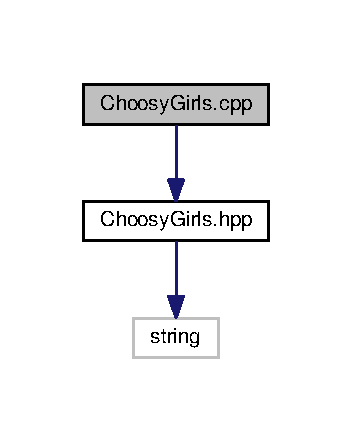
\includegraphics[width=169pt]{ChoosyGirls_8cpp__incl}
\end{center}
\end{figure}

\hypertarget{ChoosyGirls_8hpp}{}\section{Choosy\+Girls.\+hpp File Reference}
\label{ChoosyGirls_8hpp}\index{Choosy\+Girls.\+hpp@{Choosy\+Girls.\+hpp}}
{\ttfamily \#include $<$string$>$}\\*
Include dependency graph for Choosy\+Girls.\+hpp\+:
\nopagebreak
\begin{figure}[H]
\begin{center}
\leavevmode
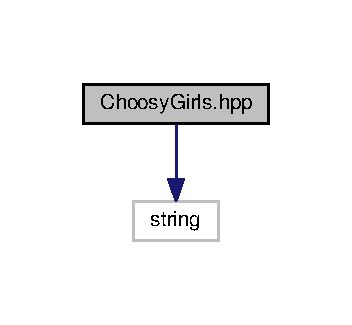
\includegraphics[width=169pt]{ChoosyGirls_8hpp__incl}
\end{center}
\end{figure}
This graph shows which files directly or indirectly include this file\+:
\nopagebreak
\begin{figure}[H]
\begin{center}
\leavevmode
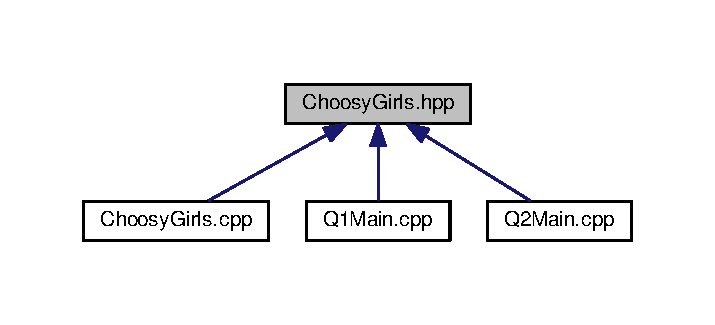
\includegraphics[width=343pt]{ChoosyGirls_8hpp__dep__incl}
\end{center}
\end{figure}
\subsection*{Classes}
\begin{DoxyCompactItemize}
\item 
class \hyperlink{classValentinePrimeTime_1_1ChoosyGirls}{Valentine\+Prime\+Time\+::\+Choosy\+Girls}
\end{DoxyCompactItemize}
\subsection*{Namespaces}
\begin{DoxyCompactItemize}
\item 
 \hyperlink{namespaceValentinePrimeTime}{Valentine\+Prime\+Time}
\end{DoxyCompactItemize}

\hypertarget{inputBoys_8txt}{}\section{data/input\+Boys.txt File Reference}
\label{inputBoys_8txt}\index{data/input\+Boys.\+txt@{data/input\+Boys.\+txt}}

\hypertarget{inputChoosyGirls_8txt}{}\section{data/input\+Choosy\+Girls.txt File Reference}
\label{inputChoosyGirls_8txt}\index{data/input\+Choosy\+Girls.\+txt@{data/input\+Choosy\+Girls.\+txt}}

\hypertarget{inputDesperateGirls_8txt}{}\section{data/input\+Desperate\+Girls.txt File Reference}
\label{inputDesperateGirls_8txt}\index{data/input\+Desperate\+Girls.\+txt@{data/input\+Desperate\+Girls.\+txt}}

\hypertarget{inputEssentialGifts_8txt}{}\section{input\+Essential\+Gifts.\+txt File Reference}
\label{inputEssentialGifts_8txt}\index{input\+Essential\+Gifts.\+txt@{input\+Essential\+Gifts.\+txt}}

\hypertarget{inputGeekBoys_8txt}{}\section{input\+Geek\+Boys.\+txt File Reference}
\label{inputGeekBoys_8txt}\index{input\+Geek\+Boys.\+txt@{input\+Geek\+Boys.\+txt}}

\hypertarget{inputGenerousBoys_8txt}{}\section{data/input\+Generous\+Boys.txt File Reference}
\label{inputGenerousBoys_8txt}\index{data/input\+Generous\+Boys.\+txt@{data/input\+Generous\+Boys.\+txt}}

\hypertarget{inputLuxuryGifts_8txt}{}\section{data/input\+Luxury\+Gifts.txt File Reference}
\label{inputLuxuryGifts_8txt}\index{data/input\+Luxury\+Gifts.\+txt@{data/input\+Luxury\+Gifts.\+txt}}

\hypertarget{inputMiserBoys_8txt}{}\section{data/input\+Miser\+Boys.txt File Reference}
\label{inputMiserBoys_8txt}\index{data/input\+Miser\+Boys.\+txt@{data/input\+Miser\+Boys.\+txt}}

\hypertarget{inputNormalGirls_8txt}{}\section{data/input\+Normal\+Girls.txt File Reference}
\label{inputNormalGirls_8txt}\index{data/input\+Normal\+Girls.\+txt@{data/input\+Normal\+Girls.\+txt}}

\hypertarget{inputUtilityGifts_8txt}{}\section{input\+Utility\+Gifts.\+txt File Reference}
\label{inputUtilityGifts_8txt}\index{input\+Utility\+Gifts.\+txt@{input\+Utility\+Gifts.\+txt}}

\hypertarget{log_8txt}{}\section{data/log.txt File Reference}
\label{log_8txt}\index{data/log.\+txt@{data/log.\+txt}}

\hypertarget{DesperateGirls_8cpp}{}\section{Desperate\+Girls.\+cpp File Reference}
\label{DesperateGirls_8cpp}\index{Desperate\+Girls.\+cpp@{Desperate\+Girls.\+cpp}}
{\ttfamily \#include \char`\"{}Desperate\+Girls.\+hpp\char`\"{}}\\*
Include dependency graph for Desperate\+Girls.\+cpp\+:
\nopagebreak
\begin{figure}[H]
\begin{center}
\leavevmode
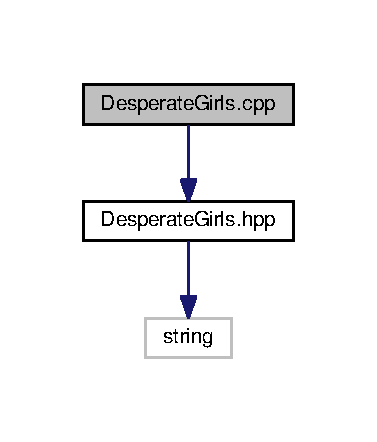
\includegraphics[width=181pt]{DesperateGirls_8cpp__incl}
\end{center}
\end{figure}

\hypertarget{DesperateGirls_8hpp}{}\section{Desperate\+Girls.\+hpp File Reference}
\label{DesperateGirls_8hpp}\index{Desperate\+Girls.\+hpp@{Desperate\+Girls.\+hpp}}
{\ttfamily \#include $<$string$>$}\\*
Include dependency graph for Desperate\+Girls.\+hpp\+:
\nopagebreak
\begin{figure}[H]
\begin{center}
\leavevmode
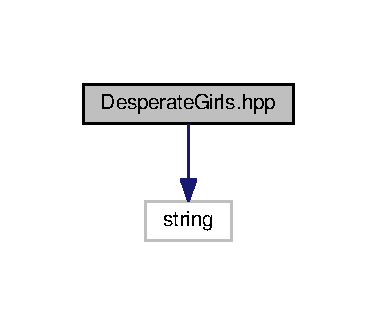
\includegraphics[width=181pt]{DesperateGirls_8hpp__incl}
\end{center}
\end{figure}
This graph shows which files directly or indirectly include this file\+:
\nopagebreak
\begin{figure}[H]
\begin{center}
\leavevmode
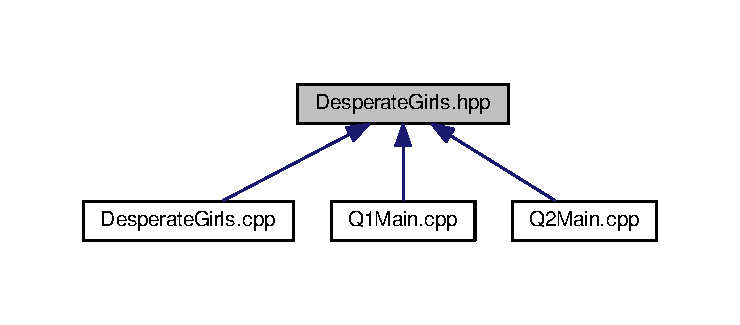
\includegraphics[width=350pt]{DesperateGirls_8hpp__dep__incl}
\end{center}
\end{figure}
\subsection*{Classes}
\begin{DoxyCompactItemize}
\item 
class \hyperlink{classValentinePrimeTime_1_1DesperateGirls}{Valentine\+Prime\+Time\+::\+Desperate\+Girls}
\end{DoxyCompactItemize}
\subsection*{Namespaces}
\begin{DoxyCompactItemize}
\item 
 \hyperlink{namespaceValentinePrimeTime}{Valentine\+Prime\+Time}
\end{DoxyCompactItemize}

\hypertarget{EssentialGifts_8cpp}{}\section{Essential\+Gifts.\+cpp File Reference}
\label{EssentialGifts_8cpp}\index{Essential\+Gifts.\+cpp@{Essential\+Gifts.\+cpp}}
{\ttfamily \#include \char`\"{}Essential\+Gifts.\+hpp\char`\"{}}\\*
Include dependency graph for Essential\+Gifts.\+cpp\+:
\nopagebreak
\begin{figure}[H]
\begin{center}
\leavevmode
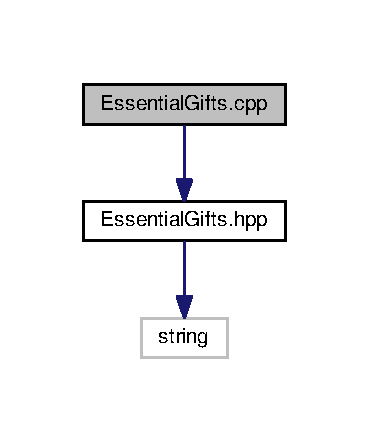
\includegraphics[width=177pt]{EssentialGifts_8cpp__incl}
\end{center}
\end{figure}

\hypertarget{EssentialGifts_8hpp}{}\section{Essential\+Gifts.\+hpp File Reference}
\label{EssentialGifts_8hpp}\index{Essential\+Gifts.\+hpp@{Essential\+Gifts.\+hpp}}
{\ttfamily \#include $<$string$>$}\\*
Include dependency graph for Essential\+Gifts.\+hpp\+:
\nopagebreak
\begin{figure}[H]
\begin{center}
\leavevmode
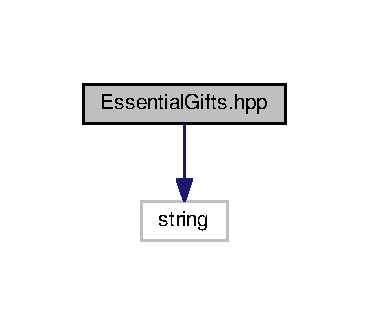
\includegraphics[width=177pt]{EssentialGifts_8hpp__incl}
\end{center}
\end{figure}
This graph shows which files directly or indirectly include this file\+:
\nopagebreak
\begin{figure}[H]
\begin{center}
\leavevmode
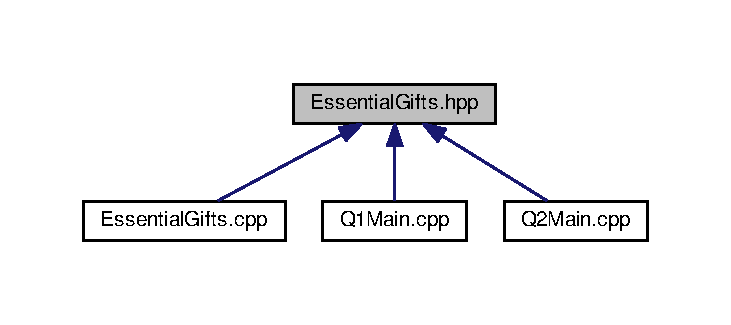
\includegraphics[width=350pt]{EssentialGifts_8hpp__dep__incl}
\end{center}
\end{figure}
\subsection*{Classes}
\begin{DoxyCompactItemize}
\item 
class \hyperlink{classValentinePrimeTime_1_1EssentialGifts}{Valentine\+Prime\+Time\+::\+Essential\+Gifts}
\end{DoxyCompactItemize}
\subsection*{Namespaces}
\begin{DoxyCompactItemize}
\item 
 \hyperlink{namespaceValentinePrimeTime}{Valentine\+Prime\+Time}
\end{DoxyCompactItemize}

\hypertarget{GeekBoys_8cpp}{}\section{Geek\+Boys.\+cpp File Reference}
\label{GeekBoys_8cpp}\index{Geek\+Boys.\+cpp@{Geek\+Boys.\+cpp}}
{\ttfamily \#include \char`\"{}Geek\+Boys.\+hpp\char`\"{}}\\*
Include dependency graph for Geek\+Boys.\+cpp\+:
\nopagebreak
\begin{figure}[H]
\begin{center}
\leavevmode
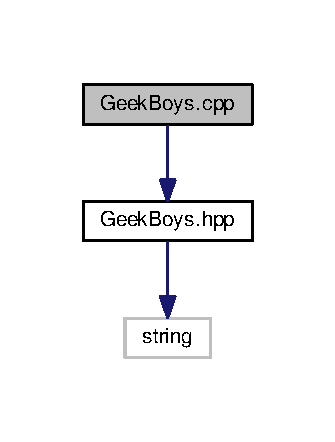
\includegraphics[width=161pt]{GeekBoys_8cpp__incl}
\end{center}
\end{figure}

\hypertarget{GeekBoys_8hpp}{}\section{Geek\+Boys.\+hpp File Reference}
\label{GeekBoys_8hpp}\index{Geek\+Boys.\+hpp@{Geek\+Boys.\+hpp}}
{\ttfamily \#include $<$string$>$}\\*
Include dependency graph for Geek\+Boys.\+hpp\+:
\nopagebreak
\begin{figure}[H]
\begin{center}
\leavevmode
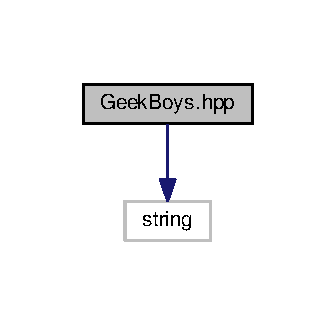
\includegraphics[width=161pt]{GeekBoys_8hpp__incl}
\end{center}
\end{figure}
This graph shows which files directly or indirectly include this file\+:
\nopagebreak
\begin{figure}[H]
\begin{center}
\leavevmode
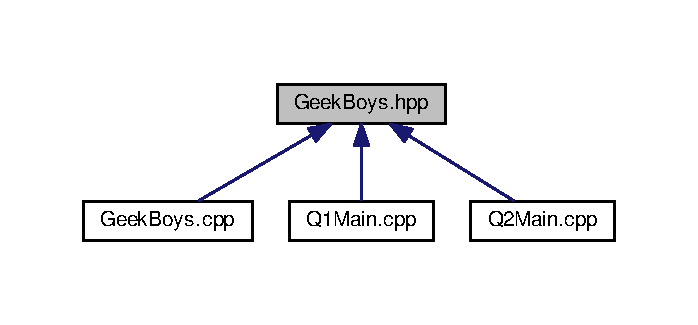
\includegraphics[width=335pt]{GeekBoys_8hpp__dep__incl}
\end{center}
\end{figure}
\subsection*{Classes}
\begin{DoxyCompactItemize}
\item 
class \hyperlink{classValentinePrimeTime_1_1GeekBoys}{Valentine\+Prime\+Time\+::\+Geek\+Boys}
\end{DoxyCompactItemize}
\subsection*{Namespaces}
\begin{DoxyCompactItemize}
\item 
 \hyperlink{namespaceValentinePrimeTime}{Valentine\+Prime\+Time}
\end{DoxyCompactItemize}

\hypertarget{GenerousBoys_8cpp}{}\section{Generous\+Boys.\+cpp File Reference}
\label{GenerousBoys_8cpp}\index{Generous\+Boys.\+cpp@{Generous\+Boys.\+cpp}}
{\ttfamily \#include \char`\"{}Generous\+Boys.\+hpp\char`\"{}}\\*
Include dependency graph for Generous\+Boys.\+cpp\+:
\nopagebreak
\begin{figure}[H]
\begin{center}
\leavevmode
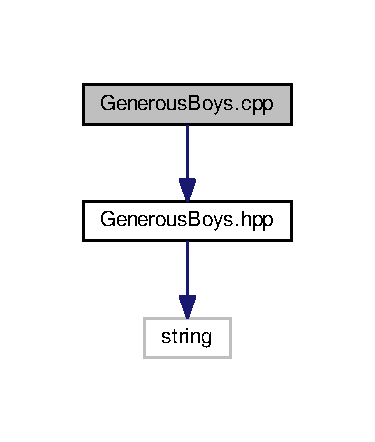
\includegraphics[width=180pt]{GenerousBoys_8cpp__incl}
\end{center}
\end{figure}

\hypertarget{GenerousBoys_8hpp}{}\section{Generous\+Boys.\+hpp File Reference}
\label{GenerousBoys_8hpp}\index{Generous\+Boys.\+hpp@{Generous\+Boys.\+hpp}}
{\ttfamily \#include $<$string$>$}\\*
Include dependency graph for Generous\+Boys.\+hpp\+:
\nopagebreak
\begin{figure}[H]
\begin{center}
\leavevmode
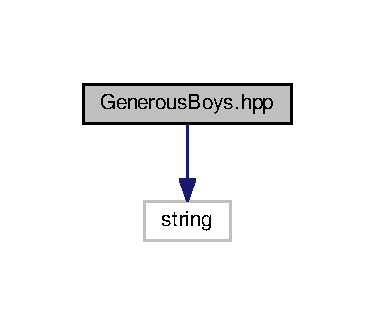
\includegraphics[width=180pt]{GenerousBoys_8hpp__incl}
\end{center}
\end{figure}
This graph shows which files directly or indirectly include this file\+:
\nopagebreak
\begin{figure}[H]
\begin{center}
\leavevmode
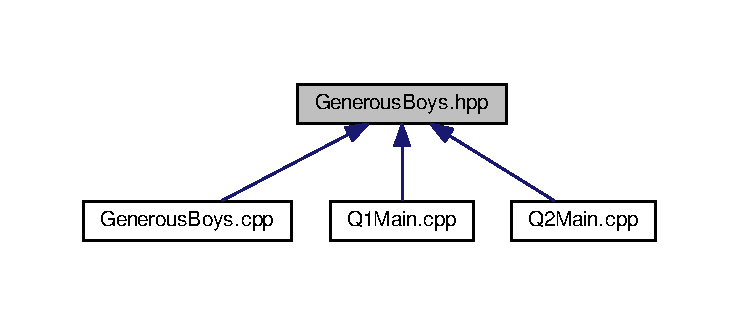
\includegraphics[width=350pt]{GenerousBoys_8hpp__dep__incl}
\end{center}
\end{figure}
\subsection*{Classes}
\begin{DoxyCompactItemize}
\item 
class \hyperlink{classValentinePrimeTime_1_1GenerousBoys}{Valentine\+Prime\+Time\+::\+Generous\+Boys}
\end{DoxyCompactItemize}
\subsection*{Namespaces}
\begin{DoxyCompactItemize}
\item 
 \hyperlink{namespaceValentinePrimeTime}{Valentine\+Prime\+Time}
\end{DoxyCompactItemize}

\hypertarget{GenTestData_8cpp}{}\section{Gen\+Test\+Data.\+cpp File Reference}
\label{GenTestData_8cpp}\index{Gen\+Test\+Data.\+cpp@{Gen\+Test\+Data.\+cpp}}
{\ttfamily \#include $<$iostream$>$}\\*
Include dependency graph for Gen\+Test\+Data.\+cpp\+:
\nopagebreak
\begin{figure}[H]
\begin{center}
\leavevmode
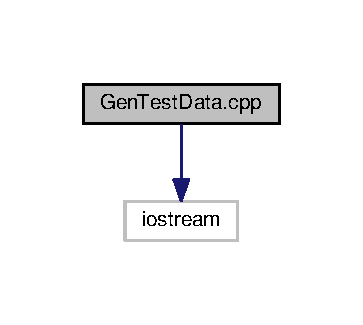
\includegraphics[width=174pt]{GenTestData_8cpp__incl}
\end{center}
\end{figure}
\subsection*{Functions}
\begin{DoxyCompactItemize}
\item 
int \hyperlink{GenTestData_8cpp_ae66f6b31b5ad750f1fe042a706a4e3d4}{main} ()
\end{DoxyCompactItemize}


\subsection{Function Documentation}
\index{Gen\+Test\+Data.\+cpp@{Gen\+Test\+Data.\+cpp}!main@{main}}
\index{main@{main}!Gen\+Test\+Data.\+cpp@{Gen\+Test\+Data.\+cpp}}
\subsubsection[{\texorpdfstring{main()}{main()}}]{\setlength{\rightskip}{0pt plus 5cm}int main (
\begin{DoxyParamCaption}
{}
\end{DoxyParamCaption}
)}\hypertarget{GenTestData_8cpp_ae66f6b31b5ad750f1fe042a706a4e3d4}{}\label{GenTestData_8cpp_ae66f6b31b5ad750f1fe042a706a4e3d4}

\hypertarget{GiftRecord_8cpp}{}\section{Gift\+Record.\+cpp File Reference}
\label{GiftRecord_8cpp}\index{Gift\+Record.\+cpp@{Gift\+Record.\+cpp}}
{\ttfamily \#include \char`\"{}Gift\+Record.\+hpp\char`\"{}}\\*
Include dependency graph for Gift\+Record.\+cpp\+:
\nopagebreak
\begin{figure}[H]
\begin{center}
\leavevmode
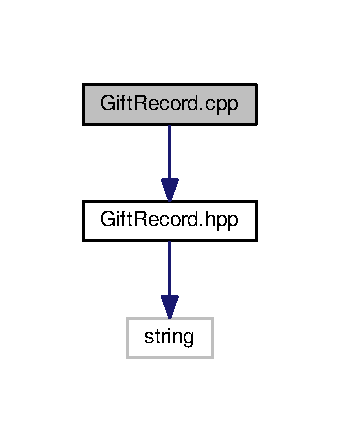
\includegraphics[width=163pt]{GiftRecord_8cpp__incl}
\end{center}
\end{figure}

\hypertarget{GiftRecord_8hpp}{}\section{Gift\+Record.\+hpp File Reference}
\label{GiftRecord_8hpp}\index{Gift\+Record.\+hpp@{Gift\+Record.\+hpp}}
{\ttfamily \#include $<$string$>$}\\*
Include dependency graph for Gift\+Record.\+hpp\+:
\nopagebreak
\begin{figure}[H]
\begin{center}
\leavevmode
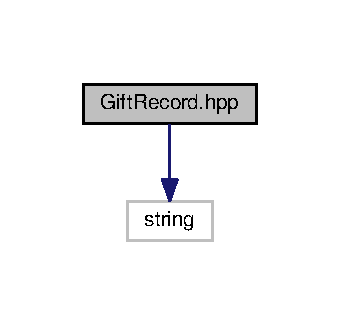
\includegraphics[width=163pt]{GiftRecord_8hpp__incl}
\end{center}
\end{figure}
This graph shows which files directly or indirectly include this file\+:
\nopagebreak
\begin{figure}[H]
\begin{center}
\leavevmode
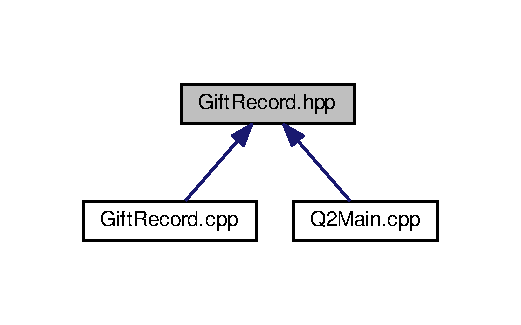
\includegraphics[width=250pt]{GiftRecord_8hpp__dep__incl}
\end{center}
\end{figure}
\subsection*{Classes}
\begin{DoxyCompactItemize}
\item 
class \hyperlink{classValentinePrimeTime_1_1GiftRecord}{Valentine\+Prime\+Time\+::\+Gift\+Record}
\end{DoxyCompactItemize}
\subsection*{Namespaces}
\begin{DoxyCompactItemize}
\item 
 \hyperlink{namespaceValentinePrimeTime}{Valentine\+Prime\+Time}
\end{DoxyCompactItemize}

\hypertarget{LuxuryGifts_8cpp}{}\section{Luxury\+Gifts.\+cpp File Reference}
\label{LuxuryGifts_8cpp}\index{Luxury\+Gifts.\+cpp@{Luxury\+Gifts.\+cpp}}
{\ttfamily \#include \char`\"{}Luxury\+Gifts.\+hpp\char`\"{}}\\*
Include dependency graph for Luxury\+Gifts.\+cpp\+:
\nopagebreak
\begin{figure}[H]
\begin{center}
\leavevmode
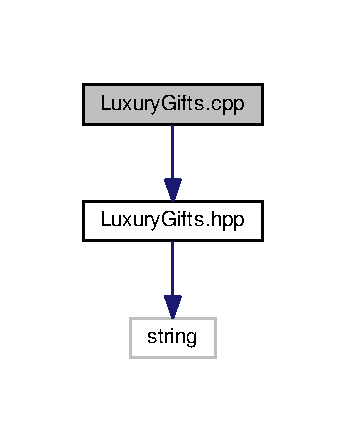
\includegraphics[width=166pt]{LuxuryGifts_8cpp__incl}
\end{center}
\end{figure}

\hypertarget{LuxuryGifts_8hpp}{}\section{Luxury\+Gifts.\+hpp File Reference}
\label{LuxuryGifts_8hpp}\index{Luxury\+Gifts.\+hpp@{Luxury\+Gifts.\+hpp}}
{\ttfamily \#include $<$string$>$}\\*
Include dependency graph for Luxury\+Gifts.\+hpp\+:
\nopagebreak
\begin{figure}[H]
\begin{center}
\leavevmode
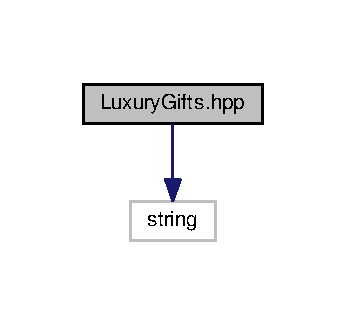
\includegraphics[width=166pt]{LuxuryGifts_8hpp__incl}
\end{center}
\end{figure}
This graph shows which files directly or indirectly include this file\+:
\nopagebreak
\begin{figure}[H]
\begin{center}
\leavevmode
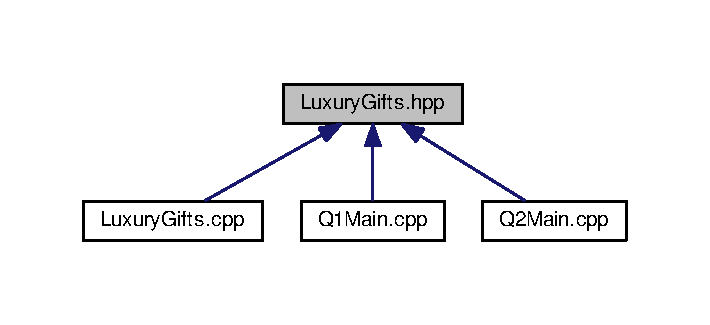
\includegraphics[width=341pt]{LuxuryGifts_8hpp__dep__incl}
\end{center}
\end{figure}
\subsection*{Classes}
\begin{DoxyCompactItemize}
\item 
class \hyperlink{classValentinePrimeTime_1_1LuxuryGifts}{Valentine\+Prime\+Time\+::\+Luxury\+Gifts}
\end{DoxyCompactItemize}
\subsection*{Namespaces}
\begin{DoxyCompactItemize}
\item 
 \hyperlink{namespaceValentinePrimeTime}{Valentine\+Prime\+Time}
\end{DoxyCompactItemize}

\hypertarget{MiserBoys_8cpp}{}\section{Miser\+Boys.\+cpp File Reference}
\label{MiserBoys_8cpp}\index{Miser\+Boys.\+cpp@{Miser\+Boys.\+cpp}}
{\ttfamily \#include \char`\"{}Miser\+Boys.\+hpp\char`\"{}}\\*
Include dependency graph for Miser\+Boys.\+cpp\+:
\nopagebreak
\begin{figure}[H]
\begin{center}
\leavevmode
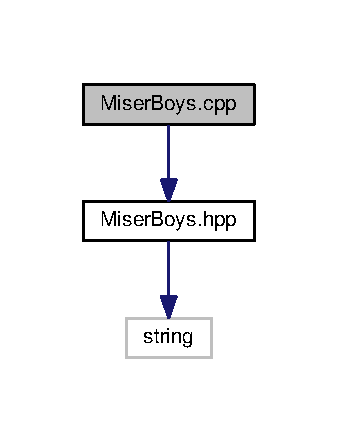
\includegraphics[width=162pt]{MiserBoys_8cpp__incl}
\end{center}
\end{figure}

\hypertarget{MiserBoys_8hpp}{}\section{Miser\+Boys.\+hpp File Reference}
\label{MiserBoys_8hpp}\index{Miser\+Boys.\+hpp@{Miser\+Boys.\+hpp}}
{\ttfamily \#include $<$string$>$}\\*
Include dependency graph for Miser\+Boys.\+hpp\+:
\nopagebreak
\begin{figure}[H]
\begin{center}
\leavevmode
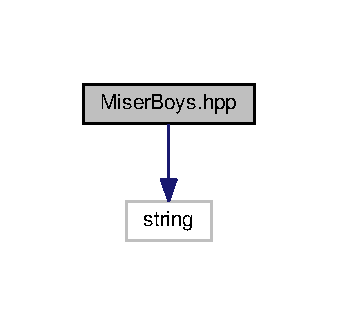
\includegraphics[width=162pt]{MiserBoys_8hpp__incl}
\end{center}
\end{figure}
This graph shows which files directly or indirectly include this file\+:
\nopagebreak
\begin{figure}[H]
\begin{center}
\leavevmode
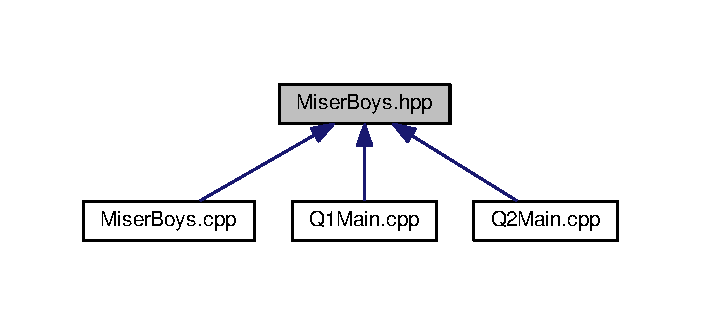
\includegraphics[width=337pt]{MiserBoys_8hpp__dep__incl}
\end{center}
\end{figure}
\subsection*{Classes}
\begin{DoxyCompactItemize}
\item 
class \hyperlink{classValentinePrimeTime_1_1MiserBoys}{Valentine\+Prime\+Time\+::\+Miser\+Boys}
\end{DoxyCompactItemize}
\subsection*{Namespaces}
\begin{DoxyCompactItemize}
\item 
 \hyperlink{namespaceValentinePrimeTime}{Valentine\+Prime\+Time}
\end{DoxyCompactItemize}

\hypertarget{NormalGirls_8cpp}{}\section{Normal\+Girls.\+cpp File Reference}
\label{NormalGirls_8cpp}\index{Normal\+Girls.\+cpp@{Normal\+Girls.\+cpp}}
{\ttfamily \#include \char`\"{}Normal\+Girls.\+hpp\char`\"{}}\\*
Include dependency graph for Normal\+Girls.\+cpp\+:
\nopagebreak
\begin{figure}[H]
\begin{center}
\leavevmode
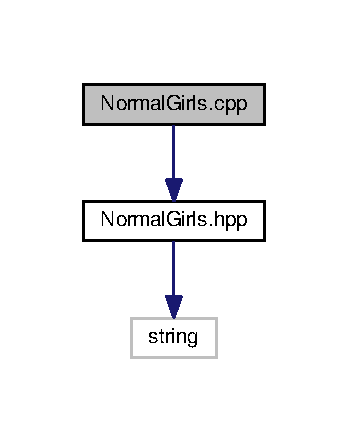
\includegraphics[width=167pt]{NormalGirls_8cpp__incl}
\end{center}
\end{figure}

\hypertarget{NormalGirls_8hpp}{}\section{Normal\+Girls.\+hpp File Reference}
\label{NormalGirls_8hpp}\index{Normal\+Girls.\+hpp@{Normal\+Girls.\+hpp}}
{\ttfamily \#include $<$string$>$}\\*
Include dependency graph for Normal\+Girls.\+hpp\+:
\nopagebreak
\begin{figure}[H]
\begin{center}
\leavevmode
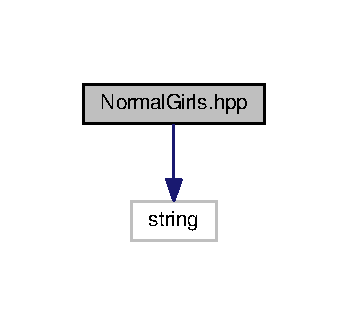
\includegraphics[width=167pt]{NormalGirls_8hpp__incl}
\end{center}
\end{figure}
This graph shows which files directly or indirectly include this file\+:
\nopagebreak
\begin{figure}[H]
\begin{center}
\leavevmode
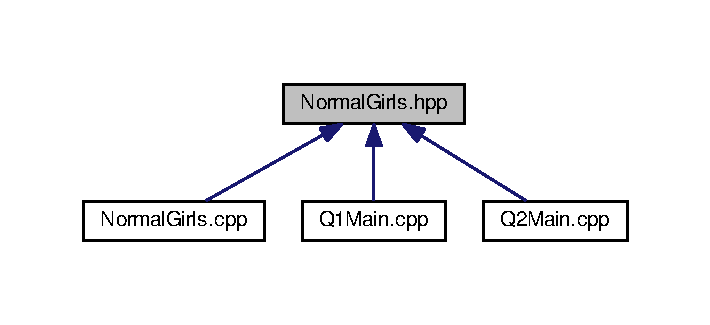
\includegraphics[width=341pt]{NormalGirls_8hpp__dep__incl}
\end{center}
\end{figure}
\subsection*{Classes}
\begin{DoxyCompactItemize}
\item 
class \hyperlink{classValentinePrimeTime_1_1NormalGirls}{Valentine\+Prime\+Time\+::\+Normal\+Girls}
\end{DoxyCompactItemize}
\subsection*{Namespaces}
\begin{DoxyCompactItemize}
\item 
 \hyperlink{namespaceValentinePrimeTime}{Valentine\+Prime\+Time}
\end{DoxyCompactItemize}

\hypertarget{Q1Main_8cpp}{}\section{Q1\+Main.\+cpp File Reference}
\label{Q1Main_8cpp}\index{Q1\+Main.\+cpp@{Q1\+Main.\+cpp}}
{\ttfamily \#include $<$iostream$>$}\\*
{\ttfamily \#include $<$fstream$>$}\\*
{\ttfamily \#include $<$algorithm$>$}\\*
{\ttfamily \#include $<$vector$>$}\\*
{\ttfamily \#include \char`\"{}Choosy\+Girls.\+hpp\char`\"{}}\\*
{\ttfamily \#include \char`\"{}Desperate\+Girls.\+hpp\char`\"{}}\\*
{\ttfamily \#include \char`\"{}Normal\+Girls.\+hpp\char`\"{}}\\*
{\ttfamily \#include \char`\"{}Miser\+Boys.\+hpp\char`\"{}}\\*
{\ttfamily \#include \char`\"{}Geek\+Boys.\+hpp\char`\"{}}\\*
{\ttfamily \#include \char`\"{}Generous\+Boys.\+hpp\char`\"{}}\\*
{\ttfamily \#include \char`\"{}Essential\+Gifts.\+hpp\char`\"{}}\\*
{\ttfamily \#include \char`\"{}Utility\+Gifts.\+hpp\char`\"{}}\\*
{\ttfamily \#include \char`\"{}Luxury\+Gifts.\+hpp\char`\"{}}\\*
{\ttfamily \#include \char`\"{}Relationship.\+hpp\char`\"{}}\\*
Include dependency graph for Q1\+Main.\+cpp\+:
\nopagebreak
\begin{figure}[H]
\begin{center}
\leavevmode
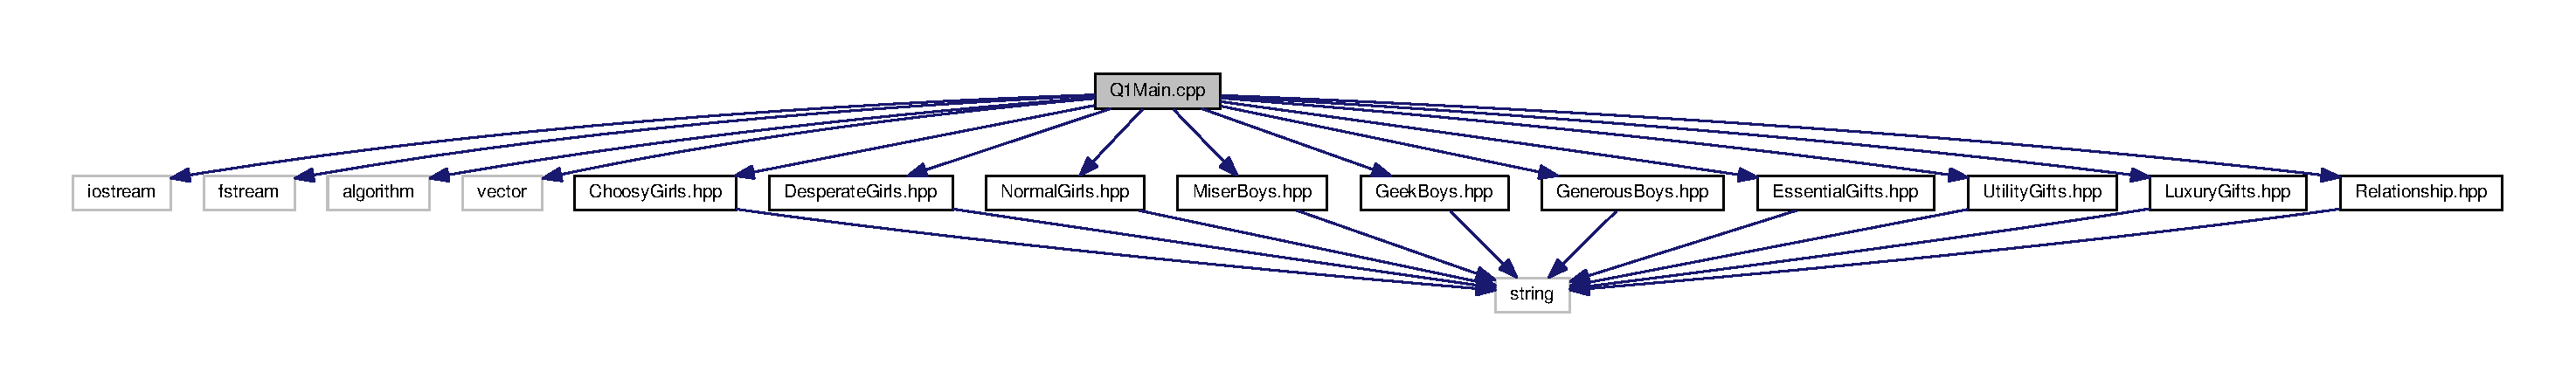
\includegraphics[width=350pt]{Q1Main_8cpp__incl}
\end{center}
\end{figure}
\subsection*{Functions}
\begin{DoxyCompactItemize}
\item 
bool \hyperlink{Q1Main_8cpp_a515b6a53a8a13a6f1c8c249233d2c31e}{essential\+Gift\+Sorter} (\hyperlink{classValentinePrimeTime_1_1EssentialGifts}{Valentine\+Prime\+Time\+::\+Essential\+Gifts} lhs, \hyperlink{classValentinePrimeTime_1_1EssentialGifts}{Valentine\+Prime\+Time\+::\+Essential\+Gifts} rhs)
\item 
bool \hyperlink{Q1Main_8cpp_a28176c143d9c5dd32d1375361804cb6a}{luxury\+Gift\+Sorter} (\hyperlink{classValentinePrimeTime_1_1LuxuryGifts}{Valentine\+Prime\+Time\+::\+Luxury\+Gifts} lhs, \hyperlink{classValentinePrimeTime_1_1LuxuryGifts}{Valentine\+Prime\+Time\+::\+Luxury\+Gifts} rhs)
\item 
bool \hyperlink{Q1Main_8cpp_a743f7ecdaa6faa9e493f3ea10f951e07}{utility\+Gift\+Sorter} (\hyperlink{classValentinePrimeTime_1_1UtilityGifts}{Valentine\+Prime\+Time\+::\+Utility\+Gifts} lhs, \hyperlink{classValentinePrimeTime_1_1UtilityGifts}{Valentine\+Prime\+Time\+::\+Utility\+Gifts} rhs)
\item 
bool \hyperlink{Q1Main_8cpp_a5821802ea2c52204c3f1f99cb0229b52}{geek\+Boys\+Sorter} (\hyperlink{classValentinePrimeTime_1_1GeekBoys}{Valentine\+Prime\+Time\+::\+Geek\+Boys} lhs, \hyperlink{classValentinePrimeTime_1_1GeekBoys}{Valentine\+Prime\+Time\+::\+Geek\+Boys} rhs)
\item 
bool \hyperlink{Q1Main_8cpp_aff72aae0792eadffe8d1825677517864}{gen\+Boys\+Sorter} (\hyperlink{classValentinePrimeTime_1_1GenerousBoys}{Valentine\+Prime\+Time\+::\+Generous\+Boys} lhs, \hyperlink{classValentinePrimeTime_1_1GenerousBoys}{Valentine\+Prime\+Time\+::\+Generous\+Boys} rhs)
\item 
bool \hyperlink{Q1Main_8cpp_a850bdb56ccb58426ad8d93a04183f99b}{miser\+Boys\+Sorter} (\hyperlink{classValentinePrimeTime_1_1MiserBoys}{Valentine\+Prime\+Time\+::\+Miser\+Boys} lhs, \hyperlink{classValentinePrimeTime_1_1MiserBoys}{Valentine\+Prime\+Time\+::\+Miser\+Boys} rhs)
\item 
int \hyperlink{Q1Main_8cpp_ae66f6b31b5ad750f1fe042a706a4e3d4}{main} ()
\end{DoxyCompactItemize}


\subsection{Function Documentation}
\index{Q1\+Main.\+cpp@{Q1\+Main.\+cpp}!essential\+Gift\+Sorter@{essential\+Gift\+Sorter}}
\index{essential\+Gift\+Sorter@{essential\+Gift\+Sorter}!Q1\+Main.\+cpp@{Q1\+Main.\+cpp}}
\subsubsection[{\texorpdfstring{essential\+Gift\+Sorter(\+Valentine\+Prime\+Time\+::\+Essential\+Gifts lhs, Valentine\+Prime\+Time\+::\+Essential\+Gifts rhs)}{essentialGiftSorter(ValentinePrimeTime::EssentialGifts lhs, ValentinePrimeTime::EssentialGifts rhs)}}]{\setlength{\rightskip}{0pt plus 5cm}bool essential\+Gift\+Sorter (
\begin{DoxyParamCaption}
\item[{{\bf Valentine\+Prime\+Time\+::\+Essential\+Gifts}}]{lhs, }
\item[{{\bf Valentine\+Prime\+Time\+::\+Essential\+Gifts}}]{rhs}
\end{DoxyParamCaption}
)}\hypertarget{Q1Main_8cpp_a515b6a53a8a13a6f1c8c249233d2c31e}{}\label{Q1Main_8cpp_a515b6a53a8a13a6f1c8c249233d2c31e}
\index{Q1\+Main.\+cpp@{Q1\+Main.\+cpp}!geek\+Boys\+Sorter@{geek\+Boys\+Sorter}}
\index{geek\+Boys\+Sorter@{geek\+Boys\+Sorter}!Q1\+Main.\+cpp@{Q1\+Main.\+cpp}}
\subsubsection[{\texorpdfstring{geek\+Boys\+Sorter(\+Valentine\+Prime\+Time\+::\+Geek\+Boys lhs, Valentine\+Prime\+Time\+::\+Geek\+Boys rhs)}{geekBoysSorter(ValentinePrimeTime::GeekBoys lhs, ValentinePrimeTime::GeekBoys rhs)}}]{\setlength{\rightskip}{0pt plus 5cm}bool geek\+Boys\+Sorter (
\begin{DoxyParamCaption}
\item[{{\bf Valentine\+Prime\+Time\+::\+Geek\+Boys}}]{lhs, }
\item[{{\bf Valentine\+Prime\+Time\+::\+Geek\+Boys}}]{rhs}
\end{DoxyParamCaption}
)}\hypertarget{Q1Main_8cpp_a5821802ea2c52204c3f1f99cb0229b52}{}\label{Q1Main_8cpp_a5821802ea2c52204c3f1f99cb0229b52}
\index{Q1\+Main.\+cpp@{Q1\+Main.\+cpp}!gen\+Boys\+Sorter@{gen\+Boys\+Sorter}}
\index{gen\+Boys\+Sorter@{gen\+Boys\+Sorter}!Q1\+Main.\+cpp@{Q1\+Main.\+cpp}}
\subsubsection[{\texorpdfstring{gen\+Boys\+Sorter(\+Valentine\+Prime\+Time\+::\+Generous\+Boys lhs, Valentine\+Prime\+Time\+::\+Generous\+Boys rhs)}{genBoysSorter(ValentinePrimeTime::GenerousBoys lhs, ValentinePrimeTime::GenerousBoys rhs)}}]{\setlength{\rightskip}{0pt plus 5cm}bool gen\+Boys\+Sorter (
\begin{DoxyParamCaption}
\item[{{\bf Valentine\+Prime\+Time\+::\+Generous\+Boys}}]{lhs, }
\item[{{\bf Valentine\+Prime\+Time\+::\+Generous\+Boys}}]{rhs}
\end{DoxyParamCaption}
)}\hypertarget{Q1Main_8cpp_aff72aae0792eadffe8d1825677517864}{}\label{Q1Main_8cpp_aff72aae0792eadffe8d1825677517864}
\index{Q1\+Main.\+cpp@{Q1\+Main.\+cpp}!luxury\+Gift\+Sorter@{luxury\+Gift\+Sorter}}
\index{luxury\+Gift\+Sorter@{luxury\+Gift\+Sorter}!Q1\+Main.\+cpp@{Q1\+Main.\+cpp}}
\subsubsection[{\texorpdfstring{luxury\+Gift\+Sorter(\+Valentine\+Prime\+Time\+::\+Luxury\+Gifts lhs, Valentine\+Prime\+Time\+::\+Luxury\+Gifts rhs)}{luxuryGiftSorter(ValentinePrimeTime::LuxuryGifts lhs, ValentinePrimeTime::LuxuryGifts rhs)}}]{\setlength{\rightskip}{0pt plus 5cm}bool luxury\+Gift\+Sorter (
\begin{DoxyParamCaption}
\item[{{\bf Valentine\+Prime\+Time\+::\+Luxury\+Gifts}}]{lhs, }
\item[{{\bf Valentine\+Prime\+Time\+::\+Luxury\+Gifts}}]{rhs}
\end{DoxyParamCaption}
)}\hypertarget{Q1Main_8cpp_a28176c143d9c5dd32d1375361804cb6a}{}\label{Q1Main_8cpp_a28176c143d9c5dd32d1375361804cb6a}
\index{Q1\+Main.\+cpp@{Q1\+Main.\+cpp}!main@{main}}
\index{main@{main}!Q1\+Main.\+cpp@{Q1\+Main.\+cpp}}
\subsubsection[{\texorpdfstring{main()}{main()}}]{\setlength{\rightskip}{0pt plus 5cm}int main (
\begin{DoxyParamCaption}
{}
\end{DoxyParamCaption}
)}\hypertarget{Q1Main_8cpp_ae66f6b31b5ad750f1fe042a706a4e3d4}{}\label{Q1Main_8cpp_ae66f6b31b5ad750f1fe042a706a4e3d4}
\index{Q1\+Main.\+cpp@{Q1\+Main.\+cpp}!miser\+Boys\+Sorter@{miser\+Boys\+Sorter}}
\index{miser\+Boys\+Sorter@{miser\+Boys\+Sorter}!Q1\+Main.\+cpp@{Q1\+Main.\+cpp}}
\subsubsection[{\texorpdfstring{miser\+Boys\+Sorter(\+Valentine\+Prime\+Time\+::\+Miser\+Boys lhs, Valentine\+Prime\+Time\+::\+Miser\+Boys rhs)}{miserBoysSorter(ValentinePrimeTime::MiserBoys lhs, ValentinePrimeTime::MiserBoys rhs)}}]{\setlength{\rightskip}{0pt plus 5cm}bool miser\+Boys\+Sorter (
\begin{DoxyParamCaption}
\item[{{\bf Valentine\+Prime\+Time\+::\+Miser\+Boys}}]{lhs, }
\item[{{\bf Valentine\+Prime\+Time\+::\+Miser\+Boys}}]{rhs}
\end{DoxyParamCaption}
)}\hypertarget{Q1Main_8cpp_a850bdb56ccb58426ad8d93a04183f99b}{}\label{Q1Main_8cpp_a850bdb56ccb58426ad8d93a04183f99b}
\index{Q1\+Main.\+cpp@{Q1\+Main.\+cpp}!utility\+Gift\+Sorter@{utility\+Gift\+Sorter}}
\index{utility\+Gift\+Sorter@{utility\+Gift\+Sorter}!Q1\+Main.\+cpp@{Q1\+Main.\+cpp}}
\subsubsection[{\texorpdfstring{utility\+Gift\+Sorter(\+Valentine\+Prime\+Time\+::\+Utility\+Gifts lhs, Valentine\+Prime\+Time\+::\+Utility\+Gifts rhs)}{utilityGiftSorter(ValentinePrimeTime::UtilityGifts lhs, ValentinePrimeTime::UtilityGifts rhs)}}]{\setlength{\rightskip}{0pt plus 5cm}bool utility\+Gift\+Sorter (
\begin{DoxyParamCaption}
\item[{{\bf Valentine\+Prime\+Time\+::\+Utility\+Gifts}}]{lhs, }
\item[{{\bf Valentine\+Prime\+Time\+::\+Utility\+Gifts}}]{rhs}
\end{DoxyParamCaption}
)}\hypertarget{Q1Main_8cpp_a743f7ecdaa6faa9e493f3ea10f951e07}{}\label{Q1Main_8cpp_a743f7ecdaa6faa9e493f3ea10f951e07}

\hypertarget{Q2Main_8cpp}{}\section{Q2\+Main.\+cpp File Reference}
\label{Q2Main_8cpp}\index{Q2\+Main.\+cpp@{Q2\+Main.\+cpp}}
{\ttfamily \#include $<$iostream$>$}\\*
{\ttfamily \#include $<$fstream$>$}\\*
{\ttfamily \#include $<$algorithm$>$}\\*
{\ttfamily \#include $<$vector$>$}\\*
{\ttfamily \#include \char`\"{}Choosy\+Girls.\+hpp\char`\"{}}\\*
{\ttfamily \#include \char`\"{}Desperate\+Girls.\+hpp\char`\"{}}\\*
{\ttfamily \#include \char`\"{}Normal\+Girls.\+hpp\char`\"{}}\\*
{\ttfamily \#include \char`\"{}Miser\+Boys.\+hpp\char`\"{}}\\*
{\ttfamily \#include \char`\"{}Geek\+Boys.\+hpp\char`\"{}}\\*
{\ttfamily \#include \char`\"{}Generous\+Boys.\+hpp\char`\"{}}\\*
{\ttfamily \#include \char`\"{}Essential\+Gifts.\+hpp\char`\"{}}\\*
{\ttfamily \#include \char`\"{}Utility\+Gifts.\+hpp\char`\"{}}\\*
{\ttfamily \#include \char`\"{}Luxury\+Gifts.\+hpp\char`\"{}}\\*
{\ttfamily \#include \char`\"{}Relationship.\+hpp\char`\"{}}\\*
{\ttfamily \#include \char`\"{}Gift\+Record.\+hpp\char`\"{}}\\*
Include dependency graph for Q2\+Main.\+cpp\+:
\nopagebreak
\begin{figure}[H]
\begin{center}
\leavevmode
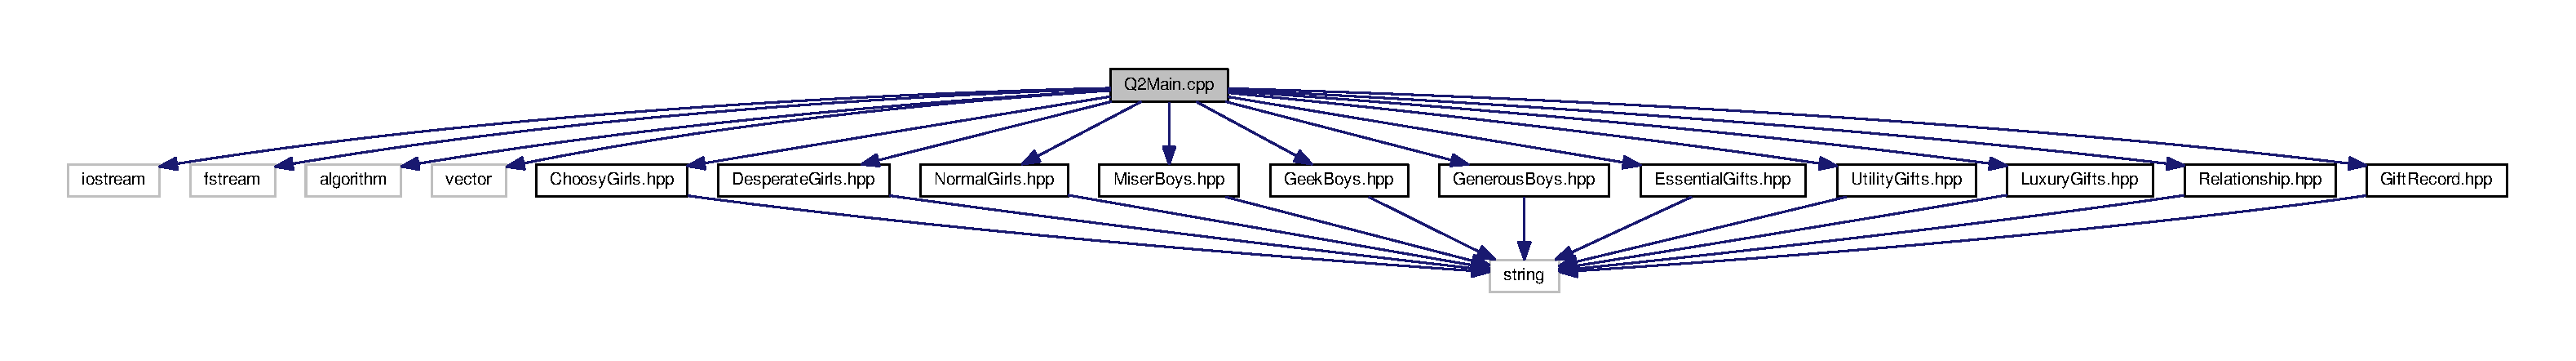
\includegraphics[width=350pt]{Q2Main_8cpp__incl}
\end{center}
\end{figure}
\subsection*{Functions}
\begin{DoxyCompactItemize}
\item 
bool \hyperlink{Q2Main_8cpp_a515b6a53a8a13a6f1c8c249233d2c31e}{essential\+Gift\+Sorter} (\hyperlink{classValentinePrimeTime_1_1EssentialGifts}{Valentine\+Prime\+Time\+::\+Essential\+Gifts} lhs, \hyperlink{classValentinePrimeTime_1_1EssentialGifts}{Valentine\+Prime\+Time\+::\+Essential\+Gifts} rhs)
\item 
bool \hyperlink{Q2Main_8cpp_a28176c143d9c5dd32d1375361804cb6a}{luxury\+Gift\+Sorter} (\hyperlink{classValentinePrimeTime_1_1LuxuryGifts}{Valentine\+Prime\+Time\+::\+Luxury\+Gifts} lhs, \hyperlink{classValentinePrimeTime_1_1LuxuryGifts}{Valentine\+Prime\+Time\+::\+Luxury\+Gifts} rhs)
\item 
bool \hyperlink{Q2Main_8cpp_a743f7ecdaa6faa9e493f3ea10f951e07}{utility\+Gift\+Sorter} (\hyperlink{classValentinePrimeTime_1_1UtilityGifts}{Valentine\+Prime\+Time\+::\+Utility\+Gifts} lhs, \hyperlink{classValentinePrimeTime_1_1UtilityGifts}{Valentine\+Prime\+Time\+::\+Utility\+Gifts} rhs)
\item 
bool \hyperlink{Q2Main_8cpp_a5821802ea2c52204c3f1f99cb0229b52}{geek\+Boys\+Sorter} (\hyperlink{classValentinePrimeTime_1_1GeekBoys}{Valentine\+Prime\+Time\+::\+Geek\+Boys} lhs, \hyperlink{classValentinePrimeTime_1_1GeekBoys}{Valentine\+Prime\+Time\+::\+Geek\+Boys} rhs)
\item 
bool \hyperlink{Q2Main_8cpp_aff72aae0792eadffe8d1825677517864}{gen\+Boys\+Sorter} (\hyperlink{classValentinePrimeTime_1_1GenerousBoys}{Valentine\+Prime\+Time\+::\+Generous\+Boys} lhs, \hyperlink{classValentinePrimeTime_1_1GenerousBoys}{Valentine\+Prime\+Time\+::\+Generous\+Boys} rhs)
\item 
bool \hyperlink{Q2Main_8cpp_a850bdb56ccb58426ad8d93a04183f99b}{miser\+Boys\+Sorter} (\hyperlink{classValentinePrimeTime_1_1MiserBoys}{Valentine\+Prime\+Time\+::\+Miser\+Boys} lhs, \hyperlink{classValentinePrimeTime_1_1MiserBoys}{Valentine\+Prime\+Time\+::\+Miser\+Boys} rhs)
\item 
bool \hyperlink{Q2Main_8cpp_a9d9a31d42f0f7d53ee0089e4e6a8d1a2}{compatibility\+Sorter} (\hyperlink{classValentinePrimeTime_1_1Relationship}{Valentine\+Prime\+Time\+::\+Relationship} lhs, \hyperlink{classValentinePrimeTime_1_1Relationship}{Valentine\+Prime\+Time\+::\+Relationship} rhs)
\item 
bool \hyperlink{Q2Main_8cpp_a5e6d8c071855e8e60c207419ad450af3}{happiness\+Sorter} (\hyperlink{classValentinePrimeTime_1_1Relationship}{Valentine\+Prime\+Time\+::\+Relationship} lhs, \hyperlink{classValentinePrimeTime_1_1Relationship}{Valentine\+Prime\+Time\+::\+Relationship} rhs)
\item 
int \hyperlink{Q2Main_8cpp_aef6304233951c1af2210d60db0d87c95}{total\+Gift\+Cost} (string boy\+Name, string girl\+Name, int budget, int $\ast$value, vector$<$ \hyperlink{classValentinePrimeTime_1_1UtilityGifts}{Valentine\+Prime\+Time\+::\+Utility\+Gifts} $>$ U, vector$<$ \hyperlink{classValentinePrimeTime_1_1EssentialGifts}{Valentine\+Prime\+Time\+::\+Essential\+Gifts} $>$ E, vector$<$ \hyperlink{classValentinePrimeTime_1_1LuxuryGifts}{Valentine\+Prime\+Time\+::\+Luxury\+Gifts} $>$ L, vector$<$ \hyperlink{classValentinePrimeTime_1_1GiftRecord}{Valentine\+Prime\+Time\+::\+Gift\+Record} $>$ $\ast$GR)
\item 
int \hyperlink{Q2Main_8cpp_ae66f6b31b5ad750f1fe042a706a4e3d4}{main} ()
\end{DoxyCompactItemize}


\subsection{Function Documentation}
\index{Q2\+Main.\+cpp@{Q2\+Main.\+cpp}!compatibility\+Sorter@{compatibility\+Sorter}}
\index{compatibility\+Sorter@{compatibility\+Sorter}!Q2\+Main.\+cpp@{Q2\+Main.\+cpp}}
\subsubsection[{\texorpdfstring{compatibility\+Sorter(\+Valentine\+Prime\+Time\+::\+Relationship lhs, Valentine\+Prime\+Time\+::\+Relationship rhs)}{compatibilitySorter(ValentinePrimeTime::Relationship lhs, ValentinePrimeTime::Relationship rhs)}}]{\setlength{\rightskip}{0pt plus 5cm}bool compatibility\+Sorter (
\begin{DoxyParamCaption}
\item[{{\bf Valentine\+Prime\+Time\+::\+Relationship}}]{lhs, }
\item[{{\bf Valentine\+Prime\+Time\+::\+Relationship}}]{rhs}
\end{DoxyParamCaption}
)}\hypertarget{Q2Main_8cpp_a9d9a31d42f0f7d53ee0089e4e6a8d1a2}{}\label{Q2Main_8cpp_a9d9a31d42f0f7d53ee0089e4e6a8d1a2}
\index{Q2\+Main.\+cpp@{Q2\+Main.\+cpp}!essential\+Gift\+Sorter@{essential\+Gift\+Sorter}}
\index{essential\+Gift\+Sorter@{essential\+Gift\+Sorter}!Q2\+Main.\+cpp@{Q2\+Main.\+cpp}}
\subsubsection[{\texorpdfstring{essential\+Gift\+Sorter(\+Valentine\+Prime\+Time\+::\+Essential\+Gifts lhs, Valentine\+Prime\+Time\+::\+Essential\+Gifts rhs)}{essentialGiftSorter(ValentinePrimeTime::EssentialGifts lhs, ValentinePrimeTime::EssentialGifts rhs)}}]{\setlength{\rightskip}{0pt plus 5cm}bool essential\+Gift\+Sorter (
\begin{DoxyParamCaption}
\item[{{\bf Valentine\+Prime\+Time\+::\+Essential\+Gifts}}]{lhs, }
\item[{{\bf Valentine\+Prime\+Time\+::\+Essential\+Gifts}}]{rhs}
\end{DoxyParamCaption}
)}\hypertarget{Q2Main_8cpp_a515b6a53a8a13a6f1c8c249233d2c31e}{}\label{Q2Main_8cpp_a515b6a53a8a13a6f1c8c249233d2c31e}
\index{Q2\+Main.\+cpp@{Q2\+Main.\+cpp}!geek\+Boys\+Sorter@{geek\+Boys\+Sorter}}
\index{geek\+Boys\+Sorter@{geek\+Boys\+Sorter}!Q2\+Main.\+cpp@{Q2\+Main.\+cpp}}
\subsubsection[{\texorpdfstring{geek\+Boys\+Sorter(\+Valentine\+Prime\+Time\+::\+Geek\+Boys lhs, Valentine\+Prime\+Time\+::\+Geek\+Boys rhs)}{geekBoysSorter(ValentinePrimeTime::GeekBoys lhs, ValentinePrimeTime::GeekBoys rhs)}}]{\setlength{\rightskip}{0pt plus 5cm}bool geek\+Boys\+Sorter (
\begin{DoxyParamCaption}
\item[{{\bf Valentine\+Prime\+Time\+::\+Geek\+Boys}}]{lhs, }
\item[{{\bf Valentine\+Prime\+Time\+::\+Geek\+Boys}}]{rhs}
\end{DoxyParamCaption}
)}\hypertarget{Q2Main_8cpp_a5821802ea2c52204c3f1f99cb0229b52}{}\label{Q2Main_8cpp_a5821802ea2c52204c3f1f99cb0229b52}
\index{Q2\+Main.\+cpp@{Q2\+Main.\+cpp}!gen\+Boys\+Sorter@{gen\+Boys\+Sorter}}
\index{gen\+Boys\+Sorter@{gen\+Boys\+Sorter}!Q2\+Main.\+cpp@{Q2\+Main.\+cpp}}
\subsubsection[{\texorpdfstring{gen\+Boys\+Sorter(\+Valentine\+Prime\+Time\+::\+Generous\+Boys lhs, Valentine\+Prime\+Time\+::\+Generous\+Boys rhs)}{genBoysSorter(ValentinePrimeTime::GenerousBoys lhs, ValentinePrimeTime::GenerousBoys rhs)}}]{\setlength{\rightskip}{0pt plus 5cm}bool gen\+Boys\+Sorter (
\begin{DoxyParamCaption}
\item[{{\bf Valentine\+Prime\+Time\+::\+Generous\+Boys}}]{lhs, }
\item[{{\bf Valentine\+Prime\+Time\+::\+Generous\+Boys}}]{rhs}
\end{DoxyParamCaption}
)}\hypertarget{Q2Main_8cpp_aff72aae0792eadffe8d1825677517864}{}\label{Q2Main_8cpp_aff72aae0792eadffe8d1825677517864}
\index{Q2\+Main.\+cpp@{Q2\+Main.\+cpp}!happiness\+Sorter@{happiness\+Sorter}}
\index{happiness\+Sorter@{happiness\+Sorter}!Q2\+Main.\+cpp@{Q2\+Main.\+cpp}}
\subsubsection[{\texorpdfstring{happiness\+Sorter(\+Valentine\+Prime\+Time\+::\+Relationship lhs, Valentine\+Prime\+Time\+::\+Relationship rhs)}{happinessSorter(ValentinePrimeTime::Relationship lhs, ValentinePrimeTime::Relationship rhs)}}]{\setlength{\rightskip}{0pt plus 5cm}bool happiness\+Sorter (
\begin{DoxyParamCaption}
\item[{{\bf Valentine\+Prime\+Time\+::\+Relationship}}]{lhs, }
\item[{{\bf Valentine\+Prime\+Time\+::\+Relationship}}]{rhs}
\end{DoxyParamCaption}
)}\hypertarget{Q2Main_8cpp_a5e6d8c071855e8e60c207419ad450af3}{}\label{Q2Main_8cpp_a5e6d8c071855e8e60c207419ad450af3}
\index{Q2\+Main.\+cpp@{Q2\+Main.\+cpp}!luxury\+Gift\+Sorter@{luxury\+Gift\+Sorter}}
\index{luxury\+Gift\+Sorter@{luxury\+Gift\+Sorter}!Q2\+Main.\+cpp@{Q2\+Main.\+cpp}}
\subsubsection[{\texorpdfstring{luxury\+Gift\+Sorter(\+Valentine\+Prime\+Time\+::\+Luxury\+Gifts lhs, Valentine\+Prime\+Time\+::\+Luxury\+Gifts rhs)}{luxuryGiftSorter(ValentinePrimeTime::LuxuryGifts lhs, ValentinePrimeTime::LuxuryGifts rhs)}}]{\setlength{\rightskip}{0pt plus 5cm}bool luxury\+Gift\+Sorter (
\begin{DoxyParamCaption}
\item[{{\bf Valentine\+Prime\+Time\+::\+Luxury\+Gifts}}]{lhs, }
\item[{{\bf Valentine\+Prime\+Time\+::\+Luxury\+Gifts}}]{rhs}
\end{DoxyParamCaption}
)}\hypertarget{Q2Main_8cpp_a28176c143d9c5dd32d1375361804cb6a}{}\label{Q2Main_8cpp_a28176c143d9c5dd32d1375361804cb6a}
\index{Q2\+Main.\+cpp@{Q2\+Main.\+cpp}!main@{main}}
\index{main@{main}!Q2\+Main.\+cpp@{Q2\+Main.\+cpp}}
\subsubsection[{\texorpdfstring{main()}{main()}}]{\setlength{\rightskip}{0pt plus 5cm}int main (
\begin{DoxyParamCaption}
{}
\end{DoxyParamCaption}
)}\hypertarget{Q2Main_8cpp_ae66f6b31b5ad750f1fe042a706a4e3d4}{}\label{Q2Main_8cpp_ae66f6b31b5ad750f1fe042a706a4e3d4}
\index{Q2\+Main.\+cpp@{Q2\+Main.\+cpp}!miser\+Boys\+Sorter@{miser\+Boys\+Sorter}}
\index{miser\+Boys\+Sorter@{miser\+Boys\+Sorter}!Q2\+Main.\+cpp@{Q2\+Main.\+cpp}}
\subsubsection[{\texorpdfstring{miser\+Boys\+Sorter(\+Valentine\+Prime\+Time\+::\+Miser\+Boys lhs, Valentine\+Prime\+Time\+::\+Miser\+Boys rhs)}{miserBoysSorter(ValentinePrimeTime::MiserBoys lhs, ValentinePrimeTime::MiserBoys rhs)}}]{\setlength{\rightskip}{0pt plus 5cm}bool miser\+Boys\+Sorter (
\begin{DoxyParamCaption}
\item[{{\bf Valentine\+Prime\+Time\+::\+Miser\+Boys}}]{lhs, }
\item[{{\bf Valentine\+Prime\+Time\+::\+Miser\+Boys}}]{rhs}
\end{DoxyParamCaption}
)}\hypertarget{Q2Main_8cpp_a850bdb56ccb58426ad8d93a04183f99b}{}\label{Q2Main_8cpp_a850bdb56ccb58426ad8d93a04183f99b}
\index{Q2\+Main.\+cpp@{Q2\+Main.\+cpp}!total\+Gift\+Cost@{total\+Gift\+Cost}}
\index{total\+Gift\+Cost@{total\+Gift\+Cost}!Q2\+Main.\+cpp@{Q2\+Main.\+cpp}}
\subsubsection[{\texorpdfstring{total\+Gift\+Cost(string boy\+Name, string girl\+Name, int budget, int $\ast$value, vector$<$ Valentine\+Prime\+Time\+::\+Utility\+Gifts $>$ U, vector$<$ Valentine\+Prime\+Time\+::\+Essential\+Gifts $>$ E, vector$<$ Valentine\+Prime\+Time\+::\+Luxury\+Gifts $>$ L, vector$<$ Valentine\+Prime\+Time\+::\+Gift\+Record $>$ $\ast$\+G\+R)}{totalGiftCost(string boyName, string girlName, int budget, int *value, vector< ValentinePrimeTime::UtilityGifts > U, vector< ValentinePrimeTime::EssentialGifts > E, vector< ValentinePrimeTime::LuxuryGifts > L, vector< ValentinePrimeTime::GiftRecord > *GR)}}]{\setlength{\rightskip}{0pt plus 5cm}int total\+Gift\+Cost (
\begin{DoxyParamCaption}
\item[{string}]{boy\+Name, }
\item[{string}]{girl\+Name, }
\item[{int}]{budget, }
\item[{int $\ast$}]{value, }
\item[{vector$<$ {\bf Valentine\+Prime\+Time\+::\+Utility\+Gifts} $>$}]{U, }
\item[{vector$<$ {\bf Valentine\+Prime\+Time\+::\+Essential\+Gifts} $>$}]{E, }
\item[{vector$<$ {\bf Valentine\+Prime\+Time\+::\+Luxury\+Gifts} $>$}]{L, }
\item[{vector$<$ {\bf Valentine\+Prime\+Time\+::\+Gift\+Record} $>$ $\ast$}]{GR}
\end{DoxyParamCaption}
)}\hypertarget{Q2Main_8cpp_aef6304233951c1af2210d60db0d87c95}{}\label{Q2Main_8cpp_aef6304233951c1af2210d60db0d87c95}
\index{Q2\+Main.\+cpp@{Q2\+Main.\+cpp}!utility\+Gift\+Sorter@{utility\+Gift\+Sorter}}
\index{utility\+Gift\+Sorter@{utility\+Gift\+Sorter}!Q2\+Main.\+cpp@{Q2\+Main.\+cpp}}
\subsubsection[{\texorpdfstring{utility\+Gift\+Sorter(\+Valentine\+Prime\+Time\+::\+Utility\+Gifts lhs, Valentine\+Prime\+Time\+::\+Utility\+Gifts rhs)}{utilityGiftSorter(ValentinePrimeTime::UtilityGifts lhs, ValentinePrimeTime::UtilityGifts rhs)}}]{\setlength{\rightskip}{0pt plus 5cm}bool utility\+Gift\+Sorter (
\begin{DoxyParamCaption}
\item[{{\bf Valentine\+Prime\+Time\+::\+Utility\+Gifts}}]{lhs, }
\item[{{\bf Valentine\+Prime\+Time\+::\+Utility\+Gifts}}]{rhs}
\end{DoxyParamCaption}
)}\hypertarget{Q2Main_8cpp_a743f7ecdaa6faa9e493f3ea10f951e07}{}\label{Q2Main_8cpp_a743f7ecdaa6faa9e493f3ea10f951e07}

\hypertarget{randomGen_8cpp}{}\section{random\+Gen.\+cpp File Reference}
\label{randomGen_8cpp}\index{random\+Gen.\+cpp@{random\+Gen.\+cpp}}
{\ttfamily \#include $<$iostream$>$}\\*
{\ttfamily \#include $<$cstdlib$>$}\\*
{\ttfamily \#include $<$fstream$>$}\\*
Include dependency graph for random\+Gen.\+cpp\+:
\nopagebreak
\begin{figure}[H]
\begin{center}
\leavevmode
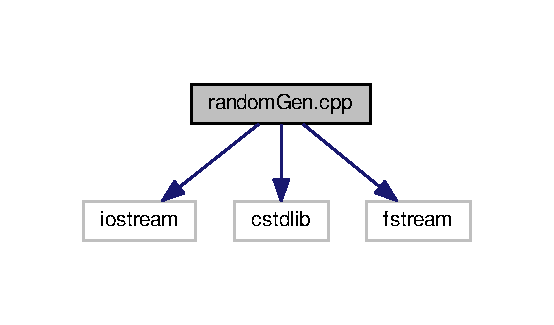
\includegraphics[width=266pt]{randomGen_8cpp__incl}
\end{center}
\end{figure}
\subsection*{Functions}
\begin{DoxyCompactItemize}
\item 
int \hyperlink{randomGen_8cpp_ae66f6b31b5ad750f1fe042a706a4e3d4}{main} ()
\end{DoxyCompactItemize}


\subsection{Function Documentation}
\index{random\+Gen.\+cpp@{random\+Gen.\+cpp}!main@{main}}
\index{main@{main}!random\+Gen.\+cpp@{random\+Gen.\+cpp}}
\subsubsection[{\texorpdfstring{main()}{main()}}]{\setlength{\rightskip}{0pt plus 5cm}int main (
\begin{DoxyParamCaption}
{}
\end{DoxyParamCaption}
)}\hypertarget{randomGen_8cpp_ae66f6b31b5ad750f1fe042a706a4e3d4}{}\label{randomGen_8cpp_ae66f6b31b5ad750f1fe042a706a4e3d4}

\hypertarget{README_8md}{}\section{R\+E\+A\+D\+M\+E.\+md File Reference}
\label{README_8md}\index{R\+E\+A\+D\+M\+E.\+md@{R\+E\+A\+D\+M\+E.\+md}}

\hypertarget{Relationship_8cpp}{}\section{Relationship.\+cpp File Reference}
\label{Relationship_8cpp}\index{Relationship.\+cpp@{Relationship.\+cpp}}
{\ttfamily \#include \char`\"{}Relationship.\+hpp\char`\"{}}\\*
Include dependency graph for Relationship.\+cpp\+:
\nopagebreak
\begin{figure}[H]
\begin{center}
\leavevmode
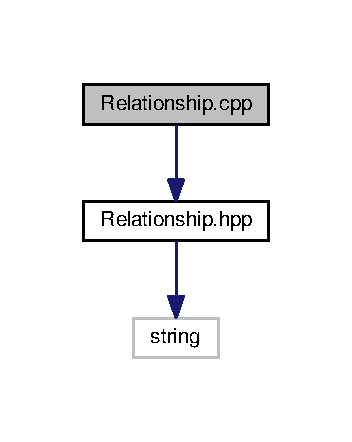
\includegraphics[width=169pt]{Relationship_8cpp__incl}
\end{center}
\end{figure}

\hypertarget{Relationship_8hpp}{}\section{Relationship.\+hpp File Reference}
\label{Relationship_8hpp}\index{Relationship.\+hpp@{Relationship.\+hpp}}
{\ttfamily \#include $<$string$>$}\\*
Include dependency graph for Relationship.\+hpp\+:
\nopagebreak
\begin{figure}[H]
\begin{center}
\leavevmode
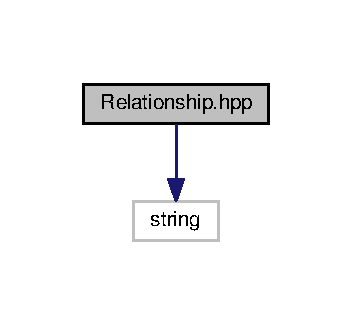
\includegraphics[width=169pt]{Relationship_8hpp__incl}
\end{center}
\end{figure}
This graph shows which files directly or indirectly include this file\+:
\nopagebreak
\begin{figure}[H]
\begin{center}
\leavevmode
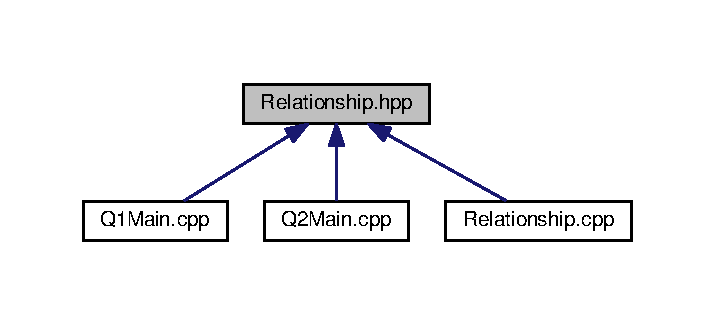
\includegraphics[width=343pt]{Relationship_8hpp__dep__incl}
\end{center}
\end{figure}
\subsection*{Classes}
\begin{DoxyCompactItemize}
\item 
class \hyperlink{classValentinePrimeTime_1_1Relationship}{Valentine\+Prime\+Time\+::\+Relationship}
\end{DoxyCompactItemize}
\subsection*{Namespaces}
\begin{DoxyCompactItemize}
\item 
 \hyperlink{namespaceValentinePrimeTime}{Valentine\+Prime\+Time}
\end{DoxyCompactItemize}

\hypertarget{UtilityGifts_8cpp}{}\section{Utility\+Gifts.\+cpp File Reference}
\label{UtilityGifts_8cpp}\index{Utility\+Gifts.\+cpp@{Utility\+Gifts.\+cpp}}
{\ttfamily \#include \char`\"{}Utility\+Gifts.\+hpp\char`\"{}}\\*
Include dependency graph for Utility\+Gifts.\+cpp\+:
\nopagebreak
\begin{figure}[H]
\begin{center}
\leavevmode
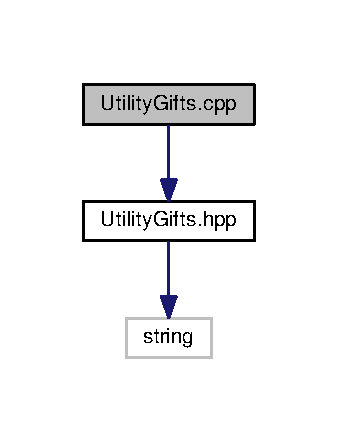
\includegraphics[width=162pt]{UtilityGifts_8cpp__incl}
\end{center}
\end{figure}

\hypertarget{UtilityGifts_8hpp}{}\section{Utility\+Gifts.\+hpp File Reference}
\label{UtilityGifts_8hpp}\index{Utility\+Gifts.\+hpp@{Utility\+Gifts.\+hpp}}
{\ttfamily \#include $<$string$>$}\\*
Include dependency graph for Utility\+Gifts.\+hpp\+:
\nopagebreak
\begin{figure}[H]
\begin{center}
\leavevmode
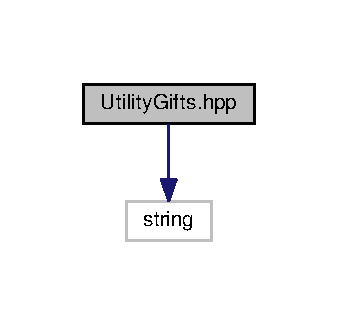
\includegraphics[width=162pt]{UtilityGifts_8hpp__incl}
\end{center}
\end{figure}
This graph shows which files directly or indirectly include this file\+:
\nopagebreak
\begin{figure}[H]
\begin{center}
\leavevmode
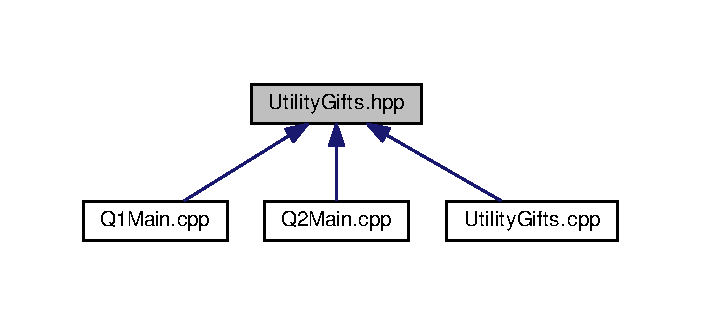
\includegraphics[width=337pt]{UtilityGifts_8hpp__dep__incl}
\end{center}
\end{figure}
\subsection*{Classes}
\begin{DoxyCompactItemize}
\item 
class \hyperlink{classValentinePrimeTime_1_1UtilityGifts}{Valentine\+Prime\+Time\+::\+Utility\+Gifts}
\end{DoxyCompactItemize}
\subsection*{Namespaces}
\begin{DoxyCompactItemize}
\item 
 \hyperlink{namespaceValentinePrimeTime}{Valentine\+Prime\+Time}
\end{DoxyCompactItemize}

%--- End generated contents ---

% Index
\backmatter
\newpage
\phantomsection
\clearemptydoublepage
\addcontentsline{toc}{chapter}{Index}
\printindex

\end{document}
